\section{Optimal Control without Feedback}\label{sec:10_2}

\subsection{Continous Time Space State Model}

Equations \cref{eq:model_se_al_pitch}-\cref{eq:model_se_al_r} can easily be written as
 \begin{equation}
     \matr{\dot{x}} = \matr{A}_c\matr{x} + \matr{B}_c\matr{u}
 \end{equation}
 by introducing the state variable $x = \begin{bmatrix}\lambda & r & p & \dot{p} \end{bmatrix}^\top$ and $u = p_{c}$.

\begin{equation}\label{eq:linear_model}
    \begin{spmatrix}{\matr{\dot{x}}}
    \dot{\lambda} \\ \dot{r} \\ \dot{p} \\ \ddot{p}
    \end{spmatrix}
    =
    \begin{spmatrix}{\matr{A}_c}
		0 & 1 & 0 & 0      \\
		0 & 0 & -K_{2} & 0 \\
		0 & 0 & 0 & 1      \\
		0 &  0 & -K_{1}K_{pp} & -K_{1}K_{pd}
	\end{spmatrix}
	\begin{spmatrix}{\matr{x}} \lambda \\ r \\ p \\ \dot{p} \end{spmatrix}
	+
	\begin{spmatrix}{\matr{B}_c}
		0 \\ 0 \\ 0 \\ K_{1}K_{pp}
	\end{spmatrix}
	p_{c}
\end{equation}

This model contains both the properties of the equations of motion governing the helicopters motion, as well as the closed loop properties of the pitch and elevation controller, which is illustrated as the control layer and the physical layer in \cref{fig:layers_openloop}.

\begin{figure}[ht]
	\centering
	\tikzset{%
  % Specifications for style of nodes:
         base/.style = {rectangle, draw = black, minimum width=5.5cm, minimum height=1.2cm}
}
\begin{tikzpicture}[node distance=2.5cm, every node/.style={fill=white}, align=center]

    \node (start)     [base]    {Model based optimization};
    \node (layer1)    [left of = start, xshift = -2.5cm] {Optimization layer};
    \node (basic)     [base, below of = start, yshift = -2.5cm] {Pitch controller (PD)
                                                              \\Elevation controller (PID)};
    \node (layer2)    [left of = basic, xshift = -2.5cm] {Basic control layer};

    \node (physical)  [base, below of = basic] {Plant (helicopter)};
    \node (layer3)    [left of = physical, xshift = -2.5cm]  {Physical layer};

    \draw[-{Latex[length = 3mm]}] ([xshift = 1.5cm]start.south west) --  node[left = .1cm,midway]{$u^*$} ([xshift = 1.5cm]basic.north west);
    %\draw[-{Latex[length = 3mm]}] ([xshift = -1cm]start.south east) -- ([xshift = -1cm]basic.north east);

    \draw[-{Latex[length = 3mm]}] (basic) -- node [left, midway] {$\begin{bmatrix} V_d \\ V_s \end{bmatrix}$} (physical);
    \draw[-{Latex[length = 3mm]}] (physical.east) --  node [above, midway] {$x$}([xshift = 2cm]physical.east);
    \draw[-{Latex[length = 3mm]}] ([xshift = .7cm]physical.east) --  ([xshift = .7cm]basic.east) -- (basic.east);


\end{tikzpicture}

	\caption{Layers in the control hierarchy (courtesy of \cite{Assignment-text})}
\label{fig:layers_openloop}
\end{figure}

\subsection{Discrete State Space Model}

To be able to integrate the state space equations into an optimization problem to be solved in matlab, we have to transform the model to a discrete form using a numerical procedure. The forward Euler method can be used to formulate a numerical solution for ODEs with a given initial value. For our model the derivation is given in \cref{eq:f_euler_1} - \cref{eq:f_euler_4}.

\begin{subequations}\label{eq:f_euler}
    \begin{align}
        \matr{x}_{n+1} = \matr{x}_n + hf(\matr{x}_n) \label{eq:f_euler_1} \\
        \matr{\dot{x}} = f(\matr{x}) \rightarrow \matr{x}_{n+1} = \matr{x}_n + h\matr{\dot{x}_n} \label{eq:f_euler_2} \\
        \matr{x}_{n+1} = \matr{x}_n + h(\matr{A}_c\matr{x}_n + \matr{B}_cu_{n}) \label{eq:f_euler_3} \\
        \matr{x}_{n+1} = (\matr{I} + h\matr{A}_c)\matr{x}_n + h\matr{B}_cu_n \label{eq:f_euler_4}
    \end{align}
\end{subequations}

\subsection{Optimal Trajectory}

Next we are going to calculate the optimal trajectory for moving from $\matr{x_{0}} = \begin{bmatrix} \lambda_{0} & 0 & 0 & 0 \end{bmatrix}^\top$ to $\matr{x_{f}} = \begin{bmatrix} \lambda_{f} & 0 & 0 & 0 \end{bmatrix}^\top$, i.e. a travel by 180 degrees. We acquire the optimal trajectory by minimizing the cost-function given in \cref{eq:cost_func}. We also include the linear constraints on the pitch reference given in \cref{eq:constraints}

\begin{equation}
    \phi = \sum_{i = 1}^{N} (\lambda_{i} - \lambda_{f})^2 + qp_{ci-1}^{2} \label{eq:cost_func}
\end{equation}

\begin{align}\label{eq:constraints}
        \mid p_k\mid\leq\frac{30\pi}{180}, \ k\in{1,...,N}
\end{align}

To use this with matlabs quadprog-function we have to rewrite the function to the form $\frac{1}{2}\matr{x^\top}\matr{Q}\matr{x} + \matr{x^\top}\matr{c}$.
\begin{subequations}\label{eq:qp_inter}
    \begin{gather}
        \phi = \frac{1}{2}\sum_{i=0}^{N-1}(\matr{x}_{i+1} - \matr{x}_{f})^\top\matr{G}(\matr{x}_{i+1} - \matr{x}_{f}) + u_{i}2qu_{i}, \\
        \matr{G} =
        \begin{pmatrix}
            2 & 0 & 0 & 0 \\
            0 & 0 & 0 & 0 \\
            0 & 0 & 0 & 0 \\
            0 & 0 & 0 & 0
        \end{pmatrix}
    \end{gather}
\end{subequations}

The discretized model given in \cref{eq:f_euler_1} - \cref{eq:f_euler_4} can be used to formulate the equality constraints for the QP-problem as seen in \cref{eq:eql_constr}.

\begin{subequations}\label{eq:eql_constr}
    \begin{gather}
        \matr{Ix}_{1} - \matr{B}u_{0} = \matr{Ax}_{0} \label{eq:eql_constr_0} \\
        \matr{Ix}_{n} -  \matr{Ax}_{n-1} - \matr{B}u_{n-1} = 0 \label{eq:eql_constr_n} \\[0.4cm]
        \begin{spmatrix}{\matr{A}_{eq}}[cccc|cccc]
            \matr{I} & \cdots & \cdots & 0 & \matr{-B} & \cdots & \cdots & 0\\
            \matr{-A} & \matr{I} &  & \vdots & 0 & \matr{-B} & & \vdots\\
            \vdots & & \ddots & \vdots & \vdots & & \ddots & \vdots\\
            0 & \cdots & \matr{-A} & \matr{I} & 0 & \cdots & \cdots  & \matr{-B}
        \end{spmatrix}
        \begin{spmatrix}{\matr{z}}
            \matr{x}_{1}    \\
            \vdots          \\
            \matr{x}_{n}    \\
            u_{0}           \\
            \vdots          \\
            u_{n-1}
        \end{spmatrix}
        =
        \begin{spmatrix}{\matr{B}_{eq}}
            \matr{Ax}_{0}   \\
            0               \\
            \vdots          \\
            \vdots          \\
            0
        \end{spmatrix}  \label{eq:eql_const_matr}
    \end{gather}
\end{subequations}

With the new introduced state variable $\matr{z}$ we can rewrite \cref{eq:qp_inter} as \cref{eq:qp_final} and solve for $N$ timesteps with quadprog. The $c$-vector is set to zero since the cost function only includes quadratic terms.

\begin{subequations}\label{eq:qp_final}
    \begin{gather}
        \phi = \frac{1}{2}\matr{z}^\top\matr{Q}\matr{z}\qquad s.t\qquad \matr{A}_{eq}\matr{z} = \matr{B}_{eq},\quad -\frac{30\pi}{180} \leq u_{n} \leq \frac{30\pi}{180}, \\[0.4cm]
        \matr{Q}=
        \begin{pmatrix}
            \matr{G} & \cdots & \matr{0} & & & \\
            \vdots & \ddots & \vdots & &  & \\
            \matr{0} & \cdots & \matr{G} & & & \\
             & & & 2q & \cdots & 0 \\
             &  & & \vdots & \ddots & \vdots \\
             & & & 0 & \cdots & 2q
        \end{pmatrix}
    \end{gather}
\end{subequations}

\vspace{0.6cm}
\subsection{Discussion and Results}
From figure \cref{fig:2_plots_q01,fig:2_plots_q1,fig:2_plots_q10} we can see that the measured travel angle $\lambda$ deviates from the calculated angle $\lambda_c$. The helicopter does travel the correct distance from $\lambda_0$ to $\lambda_f$, but is neither stationary nor in the correct absolute position. This is because there is no regulator tracking the travel angle error and correcting for it. The trajectory for travel is only estimated from its coupling with the pitch angle. Because of imperfections in the physical world, the smallest error in pitch angle will cause an increasingly large error in the travel angle (the helicopter will move at a low constant speed in the travel direction). The value $q = 1$ seems to give the best results, and is used for the remainder of the report.

\begin{figure}
    \centering
    \begin{subfigure}[t]{0.5\textwidth}
        % This file was created by matlab2tikz.
%
%The latest updates can be retrieved from
%  http://www.mathworks.com/matlabcentral/fileexchange/22022-matlab2tikz-matlab2tikz
%where you can also make suggestions and rate matlab2tikz.
%
\definecolor{mycolor1}{rgb}{0.00000,0.44700,0.74100}%
\definecolor{mycolor2}{rgb}{0.85000,0.32500,0.09800}%
%
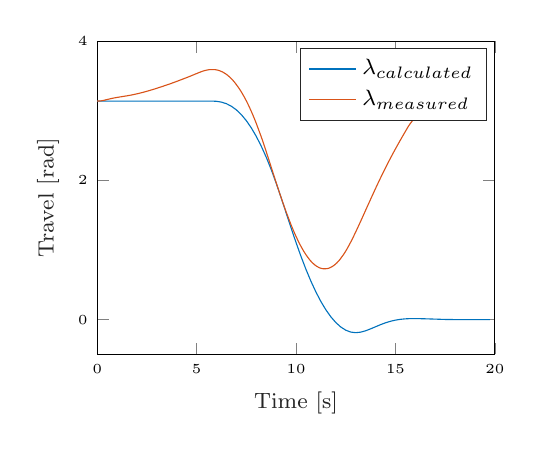
\begin{tikzpicture}

\begin{axis}[%
width=5.05cm,
height=3.975cm,
at={(0cm,0cm)},
scale only axis,
xmin=0,
xmax=20,
xlabel style={font=\color{white!15!black}},
xlabel={\footnotesize{Time [s]}},
ymin=-0.5,
ymax=4,
ylabel style={font=\color{white!15!black}},
ylabel={\footnotesize{Travel [rad]}},
ticklabel style = {font = \tiny},
axis background/.style={fill=white},
legend style={legend cell align=left, align=left, draw=white!15!black, font = \footnotesize}
]
\addplot [color=mycolor1]
  table[row sep=crcr]{%
0	3.14159265358979\\
5.75	3.14159265358979\\
6	3.13784214126101\\
6.25	3.12621555335985\\
6.5	3.10330929993986\\
6.75	3.06662741511608\\
7	3.01445392234319\\
7.25	2.94565627710196\\
7.5	2.85950776332724\\
7.75	2.75555158806609\\
8	2.6335051106824\\
8.25	2.4931956063458\\
8.5	2.33451857653721\\
8.75	2.15741132214066\\
9	1.96183648496935\\
9.25	1.75141264984868\\
9.75	1.31711679394762\\
10	1.10670906998694\\
10.25	0.907000875048698\\
10.5	0.72085629937753\\
10.75	0.550145609595759\\
11	0.396059711686981\\
11.25	0.259342846559473\\
11.5	0.140453430128577\\
11.75	0.0396705870651495\\
12	-0.0428373163003251\\
12.25	-0.10696951252422\\
12.5	-0.152666087930029\\
12.75	-0.179891622610473\\
13	-0.188625275577941\\
13.25	-0.18102987327255\\
13.5	-0.161108688690049\\
13.75	-0.133613484550949\\
14.25	-0.0731771530390617\\
14.5	-0.0465241666192924\\
14.75	-0.0246109482496557\\
15	-0.00799359542263289\\
15.25	0.00348334942129469\\
15.5	0.0104436451287633\\
15.75	0.0137606266357722\\
16	0.0143824245830935\\
16.5	0.0110062249869856\\
17.5	0.00160743307129252\\
18.25	-0.00119807103319758\\
19.5	-0.000713417108546111\\
19.75	-0.000468469183601883\\
};
\addlegendentry{$\lambda{}_{\text{calculated}}$}

\addplot [color=mycolor2]
  table[row sep=crcr]{%
0	3.14159265358979\\
0.148	3.14312663437768\\
0.154	3.14389362477162\\
0.212	3.14542760555951\\
0.218	3.14619459595345\\
0.254000000000001	3.14772857674134\\
0.260000000000002	3.14849556713528\\
0.300000000000001	3.15002954792316\\
0.306000000000001	3.15079653831711\\
0.341999999999999	3.15233051910499\\
0.350000000000001	3.15386449989288\\
0.353999999999999	3.15309750949893\\
0.361999999999998	3.15463149028682\\
0.388000000000002	3.15616547107471\\
0.391999999999999	3.15693246146865\\
0.398	3.15616547107471\\
0.405999999999999	3.15769945186259\\
0.411999999999999	3.15693246146865\\
0.420000000000002	3.15846644225654\\
0.423999999999999	3.15769945186259\\
0.431999999999999	3.15923343265048\\
0.457999999999998	3.16076741343836\\
0.462	3.16153440383231\\
0.466000000000001	3.16076741343836\\
0.474	3.16230139422625\\
0.510000000000002	3.16383537501413\\
0.518000000000001	3.16536935580202\\
0.545999999999999	3.16690333658991\\
0.552	3.16767032698385\\
0.582000000000001	3.16920430777174\\
0.588000000000001	3.16997129816568\\
0.614000000000001	3.17150527895356\\
0.620000000000001	3.17227226934751\\
0.649999999999999	3.17380625013539\\
0.655999999999999	3.17457324052933\\
0.686	3.17610722131722\\
0.692	3.17687421171116\\
0.722000000000001	3.17840819249905\\
0.728000000000002	3.17917518289299\\
0.760000000000002	3.18070916368088\\
0.766000000000002	3.18147615407482\\
0.800000000000001	3.18301013486271\\
0.806000000000001	3.18377712525665\\
0.84	3.18531110604453\\
0.846	3.18607809643848\\
0.882000000000001	3.18761207722636\\
0.888000000000002	3.18837906762031\\
0.925999999999998	3.18991304840819\\
0.931999999999999	3.19068003880214\\
0.969999999999999	3.19221401959002\\
0.975999999999999	3.19298100998396\\
1.018	3.19451499077185\\
1.024	3.19528198116579\\
1.064	3.19681596195367\\
1.07	3.19758295234762\\
1.114	3.1991169331355\\
1.12	3.19988392352945\\
1.164	3.20141790431733\\
1.17	3.20218489471128\\
1.216	3.20371887549916\\
1.222	3.2044858658931\\
1.266	3.20601984668099\\
1.272	3.20678683707493\\
1.316	3.20832081786282\\
1.322	3.20908780825676\\
1.366	3.21062178904465\\
1.372	3.21138877943859\\
1.418	3.21292276022648\\
1.424	3.21368975062042\\
1.466	3.2152237314083\\
1.472	3.21599072180225\\
1.514	3.21752470259013\\
1.52	3.21829169298407\\
1.558	3.21982567377196\\
1.564	3.2205926641659\\
1.602	3.22212664495379\\
1.608	3.22289363534773\\
1.646	3.22442761613562\\
1.652	3.22519460652956\\
1.688	3.22672858731745\\
1.694	3.22749557771139\\
1.73	3.22902955849927\\
1.736	3.22979654889322\\
1.772	3.2313305296811\\
1.778	3.23209752007505\\
1.81	3.23363150086293\\
1.816	3.23439849125688\\
1.848	3.23593247204476\\
1.854	3.2366994624387\\
1.886	3.23823344322659\\
1.892	3.23900043362053\\
1.924	3.24053441440842\\
1.93	3.24130140480236\\
1.958	3.24283538559025\\
1.964	3.24360237598419\\
1.994	3.24513635677208\\
2	3.24590334716602\\
2.028	3.2474373279539\\
2.034	3.24820431834785\\
2.062	3.24973829913573\\
2.068	3.25050528952967\\
2.094	3.25203927031756\\
2.1	3.2528062607115\\
2.128	3.25434024149939\\
2.134	3.25510723189333\\
2.16	3.25664121268122\\
2.166	3.25740820307516\\
2.192	3.25894218386305\\
2.198	3.25970917425699\\
2.224	3.26124315504487\\
2.23	3.26201014543881\\
2.256	3.2635441262267\\
2.262	3.26431111662064\\
2.286	3.26584509740853\\
2.292	3.26661208780247\\
2.318	3.26814606859036\\
2.324	3.2689130589843\\
2.348	3.27044703977219\\
2.354	3.27121403016613\\
2.378	3.27274801095401\\
2.384	3.27351500134796\\
2.406	3.27504898213584\\
2.412	3.27581597252979\\
2.436	3.27734995331767\\
2.442	3.27811694371162\\
2.466	3.2796509244995\\
2.472	3.28041791489344\\
2.494	3.28195189568133\\
2.5	3.28271888607527\\
2.524	3.28425286686316\\
2.53	3.2850198572571\\
2.552	3.28655383804499\\
2.558	3.28732082843893\\
2.58	3.28885480922682\\
2.586	3.28962179962076\\
2.606	3.29115578040864\\
2.612	3.29192277080259\\
2.634	3.29345675159047\\
2.64	3.29422374198441\\
2.662	3.2957577227723\\
2.668	3.29652471316624\\
2.688	3.29805869395413\\
2.694	3.29882568434807\\
2.714	3.30035966513596\\
2.72	3.3011266555299\\
2.742	3.30266063631779\\
2.748	3.30342762671173\\
2.77	3.30496160749961\\
2.778	3.3064955882875\\
2.804	3.30802956907539\\
2.81	3.30879655946933\\
2.83	3.31033054025722\\
2.836	3.31109753065116\\
2.856	3.31263151143904\\
2.862	3.31339850183299\\
2.882	3.31493248262087\\
2.888	3.31569947301481\\
2.908	3.3172334538027\\
2.914	3.31800044419664\\
2.932	3.31953442498453\\
2.938	3.32030141537847\\
2.958	3.32183539616636\\
2.964	3.3226023865603\\
2.984	3.32413636734818\\
2.99	3.32490335774213\\
3.01	3.32643733853001\\
3.016	3.32720432892395\\
3.034	3.32873830971184\\
3.04	3.32950530010578\\
3.06	3.33103928089367\\
3.066	3.33180627128761\\
3.084	3.3333402520755\\
3.09	3.33410724246944\\
3.11	3.33564122325733\\
3.116	3.33640821365127\\
3.134	3.33794219443915\\
3.14	3.3387091848331\\
3.158	3.34024316562098\\
3.164	3.34101015601493\\
3.184	3.34254413680281\\
3.19	3.34331112719676\\
3.208	3.34484510798464\\
3.214	3.34561209837858\\
3.232	3.34714607916647\\
3.238	3.34791306956041\\
3.256	3.3494470503483\\
3.262	3.35021404074224\\
3.28	3.35174802153013\\
3.286	3.35251501192407\\
3.306	3.35404899271196\\
3.314	3.35558297349984\\
3.338	3.35711695428773\\
3.346	3.35865093507561\\
3.37	3.3601849158635\\
3.378	3.36171889665138\\
3.4	3.36325287743927\\
3.406	3.36401986783321\\
3.424	3.3655538486211\\
3.43	3.36632083901504\\
3.448	3.36785481980293\\
3.454	3.36862181019687\\
3.472	3.37015579098475\\
3.48	3.37168977177264\\
3.502	3.37322375256052\\
3.508	3.37399074295447\\
3.526	3.37552472374236\\
3.532	3.3762917141363\\
3.55	3.37782569492418\\
3.556	3.37859268531813\\
3.572	3.38012666610601\\
3.578	3.38089365649995\\
3.594	3.38242763728784\\
3.6	3.38319462768178\\
3.618	3.38472860846967\\
3.624	3.38549559886361\\
3.64	3.3870295796515\\
3.646	3.38779657004544\\
3.664	3.38933055083332\\
3.67	3.39009754122727\\
3.686	3.39163152201515\\
3.692	3.39239851240909\\
3.71	3.39393249319698\\
3.718	3.39546647398487\\
3.74	3.39700045477275\\
3.748	3.39853443556064\\
3.77	3.40006841634852\\
3.778	3.40160239713641\\
3.8	3.40313637792429\\
3.808	3.40467035871218\\
3.83	3.40620433950007\\
3.838	3.40773832028795\\
3.858	3.40927230107584\\
3.866	3.41080628186372\\
3.888	3.41234026265161\\
3.896	3.41387424343949\\
3.918	3.41540822422738\\
3.926	3.41694220501527\\
3.946	3.41847618580315\\
3.954	3.42001016659104\\
3.976	3.42154414737892\\
3.984	3.42307812816681\\
4.004	3.42461210895469\\
4.012	3.42614608974258\\
4.034	3.42768007053046\\
4.042	3.42921405131835\\
4.062	3.43074803210624\\
4.07	3.43228201289412\\
4.09	3.43381599368201\\
4.096	3.43458298407595\\
4.112	3.43611696486384\\
4.12	3.43765094565172\\
4.14	3.43918492643961\\
4.148	3.44071890722749\\
4.168	3.44225288801538\\
4.174	3.44301987840932\\
4.19	3.44455385919721\\
4.198	3.44608783998509\\
4.218	3.44762182077298\\
4.226	3.44915580156086\\
4.246	3.45068978234875\\
4.254	3.45222376313664\\
4.274	3.45375774392452\\
4.282	3.45529172471241\\
4.302	3.45682570550029\\
4.31	3.45835968628818\\
4.33	3.45989366707606\\
4.338	3.46142764786395\\
4.358	3.46296162865184\\
4.366	3.46449560943972\\
4.384	3.46602959022761\\
4.39	3.46679658062155\\
4.406	3.46833056140943\\
4.414	3.46986454219732\\
4.434	3.47139852298521\\
4.442	3.47293250377309\\
4.46	3.47446648456098\\
4.466	3.47523347495492\\
4.482	3.47676745574281\\
4.49	3.47830143653069\\
4.508	3.47983541731858\\
4.516	3.48136939810646\\
4.536	3.48290337889435\\
4.544	3.48443735968224\\
4.562	3.48597134047012\\
4.57	3.48750532125801\\
4.588	3.48903930204589\\
4.594	3.48980629243983\\
4.61	3.49134027322772\\
4.618	3.4928742540156\\
4.636	3.49440823480349\\
4.644	3.49594221559138\\
4.662	3.49747619637926\\
4.668	3.49824318677321\\
4.682	3.49977716756109\\
4.69	3.50131114834898\\
4.708	3.50284512913686\\
4.714	3.5036121195308\\
4.728	3.50514610031869\\
4.734	3.50591309071263\\
4.748	3.50744707150052\\
4.756	3.50898105228841\\
4.776	3.51051503307629\\
4.784	3.51204901386417\\
4.802	3.51358299465206\\
4.81	3.51511697543995\\
4.828	3.51665095622783\\
4.836	3.51818493701572\\
4.854	3.5197189178036\\
4.862	3.52125289859149\\
4.88	3.52278687937937\\
4.888	3.52432086016726\\
4.906	3.52585484095515\\
4.914	3.52738882174303\\
4.932	3.52892280253092\\
4.94	3.5304567833188\\
4.958	3.53199076410669\\
4.966	3.53352474489457\\
4.984	3.53505872568246\\
4.992	3.53659270647035\\
5.01	3.53812668725823\\
5.018	3.53966066804612\\
5.036	3.541194648834\\
5.044	3.54272862962189\\
5.062	3.54426261040977\\
5.068	3.54502960080372\\
5.082	3.5465635815916\\
5.088	3.54733057198554\\
5.102	3.54886455277343\\
5.11	3.55039853356132\\
5.128	3.5519325143492\\
5.134	3.55269950474315\\
5.148	3.55423348553103\\
5.154	3.55500047592497\\
5.17	3.55653445671286\\
5.178	3.55806843750074\\
5.198	3.55960241828863\\
5.206	3.56113639907652\\
5.226	3.5626703798644\\
5.234	3.56420436065229\\
5.256	3.56573834144017\\
5.264	3.56727232222806\\
5.286	3.56880630301594\\
5.294	3.57034028380383\\
5.318	3.57187426459172\\
5.324	3.57264125498566\\
5.342	3.57417523577355\\
5.348	3.57494222616749\\
5.37	3.57647620695537\\
5.378	3.57801018774326\\
5.406	3.57954416853114\\
5.412	3.58031115892509\\
5.438	3.58184513971297\\
5.444	3.58261213010692\\
5.468	3.5841461108948\\
5.474	3.58491310128874\\
5.506	3.58644708207663\\
5.512	3.58721407247057\\
5.548	3.58874805325846\\
5.554	3.5895150436524\\
5.594	3.59104902444029\\
5.6	3.59181601483423\\
5.664	3.59334999562212\\
5.67	3.59411698601606\\
5.944	3.59258300522817\\
5.95	3.59181601483423\\
5.994	3.59028203404634\\
6	3.5895150436524\\
6.032	3.58798106286451\\
6.038	3.58721407247057\\
6.066	3.58568009168269\\
6.072	3.58491310128874\\
6.094	3.58337912050086\\
6.1	3.58261213010692\\
6.122	3.58107814931903\\
6.13	3.57954416853114\\
6.152	3.57801018774326\\
6.158	3.57724319734931\\
6.174	3.57570921656143\\
6.18	3.57494222616749\\
6.196	3.5734082453796\\
6.204	3.57187426459172\\
6.222	3.57034028380383\\
6.23	3.56880630301594\\
6.246	3.56727232222806\\
6.254	3.56573834144017\\
6.27	3.56420436065229\\
6.278	3.5626703798644\\
6.292	3.56113639907652\\
6.3	3.55960241828863\\
6.312	3.55806843750074\\
6.32	3.55653445671286\\
6.334	3.55500047592497\\
6.344	3.55269950474315\\
6.356	3.55116552395526\\
6.364	3.54963154316737\\
6.376	3.54809756237949\\
6.386	3.54579659119766\\
6.398	3.54426261040977\\
6.406	3.54272862962189\\
6.414	3.541194648834\\
6.422	3.53966066804612\\
6.432	3.53812668725823\\
6.442	3.5358257160764\\
6.452	3.53429173528852\\
6.462	3.53199076410669\\
6.472	3.5304567833188\\
6.484	3.52738882174303\\
6.494	3.52585484095515\\
6.506	3.52278687937937\\
6.516	3.52125289859149\\
6.528	3.51818493701572\\
6.538	3.51665095622783\\
6.55	3.51358299465206\\
6.558	3.51204901386417\\
6.572	3.50821406189446\\
6.58	3.50668008110658\\
6.592	3.5036121195308\\
6.6	3.50207813874292\\
6.614	3.49824318677321\\
6.622	3.49670920598532\\
6.636	3.4928742540156\\
6.644	3.49134027322772\\
6.662	3.48597134047012\\
6.67	3.48443735968224\\
6.688	3.47906842692463\\
6.696	3.47753444613675\\
6.716	3.47139852298521\\
6.722	3.46986454219732\\
6.738	3.46526259983366\\
6.744	3.46372861904578\\
6.766	3.45682570550029\\
6.772	3.45529172471241\\
6.794	3.44838881116692\\
6.8	3.44685483037903\\
6.826	3.43841793604566\\
6.832	3.43688395525778\\
6.866	3.42537909934864\\
6.872	3.42384511856075\\
6.924	3.40543734910612\\
6.93	3.40390336831824\\
7.136	3.32336937695424\\
7.142	3.32030141537847\\
7.18	3.30419461710567\\
7.186	3.3011266555299\\
7.216	3.28808781883287\\
7.222	3.2850198572571\\
7.244	3.27504898213584\\
7.25	3.27198102056007\\
7.268	3.2635441262267\\
7.274	3.26047616465093\\
7.294	3.25127227992362\\
7.302	3.24667033755996\\
7.322	3.23746645283265\\
7.33	3.23286451046899\\
7.348	3.22442761613562\\
7.356	3.21982567377196\\
7.372	3.21215576983253\\
7.378	3.20908780825676\\
7.39	3.20295188510522\\
7.398	3.19834994274156\\
7.412	3.19144702919608\\
7.42	3.18684508683242\\
7.432	3.18070916368088\\
7.44	3.17610722131722\\
7.454	3.16920430777174\\
7.464	3.16306838462019\\
7.476	3.15693246146865\\
7.484	3.15233051910499\\
7.494	3.14696158634739\\
7.504	3.14082566319585\\
7.516	3.13468974004431\\
7.526	3.12855381689277\\
7.536	3.12318488413517\\
7.546	3.11704896098362\\
7.556	3.11168002822602\\
7.566	3.10554410507448\\
7.576	3.10017517231688\\
7.586	3.09403924916534\\
7.594	3.08943730680168\\
7.604	3.08330138365014\\
7.612	3.07869944128648\\
7.624	3.07102953734706\\
7.634	3.06566060458945\\
7.646	3.05799070065003\\
7.654	3.05338875828637\\
7.668	3.04418487355905\\
7.676	3.0395829311954\\
7.688	3.03191302725597\\
7.696	3.02731108489231\\
7.712	3.01657321937711\\
7.72	3.01197127701346\\
7.734	3.00276739228614\\
7.742	2.99816544992249\\
7.76	2.9858936036194\\
7.768	2.98129166125574\\
7.788	2.96748583416477\\
7.796	2.96288389180112\\
7.818	2.94754408392226\\
7.824	2.94370913195255\\
7.842	2.93143728564946\\
7.848	2.92760233367975\\
7.87	2.91226252580089\\
7.876	2.90842757383118\\
7.902	2.89001980437655\\
7.908	2.88618485240683\\
7.94	2.86317514058855\\
7.946	2.85934018861883\\
7.988	2.82866057286112\\
7.994	2.82482562089141\\
8.25	2.62694209925416\\
8.258	2.62003918570868\\
8.29	2.59396151231462\\
8.298	2.58705859876913\\
8.326	2.56404888695085\\
8.336	2.55484500222354\\
8.366	2.53030130961736\\
8.376	2.52109742489005\\
8.4	2.50115567464754\\
8.408	2.49425276110205\\
8.424	2.48044693401108\\
8.432	2.4735440204656\\
8.45	2.45820421258674\\
8.46	2.44900032785943\\
8.478	2.43366051998057\\
8.488	2.42445663525326\\
8.506	2.4091168273744\\
8.516	2.39991294264708\\
8.532	2.38610711555611\\
8.542	2.3769032308288\\
8.56	2.36156342294995\\
8.57	2.35235953822263\\
8.584	2.34008769191955\\
8.594	2.33088380719223\\
8.608	2.31861196088915\\
8.618	2.30940807616183\\
8.634	2.29560224907086\\
8.644	2.28639836434355\\
8.658	2.27412651804046\\
8.668	2.26492263331315\\
8.68	2.25418476779795\\
8.69	2.24498088307064\\
8.706	2.23117505597967\\
8.718	2.21967020007052\\
8.734	2.20586437297955\\
8.744	2.19666048825224\\
8.758	2.18438864194915\\
8.768	2.17518475722184\\
8.782	2.16291291091876\\
8.792	2.15370902619144\\
8.806	2.14143717988836\\
8.816	2.13223329516104\\
8.83	2.11996144885796\\
8.84	2.11075756413064\\
8.854	2.09848571782756\\
8.864	2.08928183310024\\
8.878	2.07700998679716\\
8.888	2.06780610206985\\
8.902	2.05553425576676\\
8.912	2.04633037103945\\
8.928	2.03252454394848\\
8.938	2.02332065922116\\
8.954	2.00951483213019\\
8.964	2.00031094740288\\
8.98	1.9865051203119\\
8.99	1.97730123558459\\
9.006	1.96349540849362\\
9.016	1.95429152376631\\
9.034	1.93895171588745\\
9.042	1.93204880234196\\
9.058	1.91824297525099\\
9.068	1.90903909052368\\
9.088	1.89216530185694\\
9.098	1.88296141712962\\
9.118	1.86608762846288\\
9.128	1.85688374373557\\
9.15	1.83847597428094\\
9.16	1.82927208955363\\
9.184	1.80933033931111\\
9.194	1.8001264545838\\
9.22	1.7786507235534\\
9.228	1.77174781000792\\
9.25	1.75334004055329\\
9.258	1.7464371270078\\
9.282	1.72649537676529\\
9.29	1.7195924632198\\
9.318	1.69658275140152\\
9.326	1.68967983785603\\
9.356	1.66513614524986\\
9.364	1.65823323170438\\
9.406	1.62448565437089\\
9.414	1.61758274082541\\
9.476	1.56849535561307\\
9.484	1.56159244206758\\
9.696	1.40052445933959\\
9.702	1.39668950736988\\
9.746	1.36447591082428\\
9.752	1.36064095885456\\
9.782	1.33916522782416\\
9.788	1.33533027585445\\
9.814	1.31692250639982\\
9.82	1.31308755443011\\
9.842	1.29774774655125\\
9.848	1.29391279458154\\
9.866	1.28164094827845\\
9.872	1.27780599630874\\
9.888	1.26706813079354\\
9.894	1.26323317882382\\
9.91	1.25249531330862\\
9.916	1.24866036133891\\
9.93	1.2394564766116\\
9.938	1.23485453424794\\
9.956	1.22258268794486\\
9.964	1.2179807455812\\
9.978	1.20877686085388\\
9.986	1.20417491849023\\
10	1.19497103376291\\
10.008	1.19036909139926\\
10.022	1.18116520667195\\
10.03	1.17656326430829\\
10.042	1.16889336036886\\
10.052	1.16352442761126\\
10.064	1.15585452367183\\
10.072	1.15125258130817\\
10.082	1.14511665815663\\
10.09	1.14051471579297\\
10.1	1.13437879264143\\
10.11	1.12900985988383\\
10.12	1.12287393673229\\
10.13	1.11750500397469\\
10.14	1.11136908082315\\
10.15	1.10600014806555\\
10.16	1.099864224914\\
10.17	1.09449529215641\\
10.178	1.08989334979275\\
10.19	1.08375742664121\\
10.2	1.07762150348966\\
10.212	1.07148558033812\\
10.22	1.06688363797446\\
10.232	1.06074771482292\\
10.24	1.05614577245926\\
10.252	1.05000984930772\\
10.26	1.04540790694406\\
10.276	1.03773800300464\\
10.284	1.03313606064098\\
10.298	1.02623314709549\\
10.304	1.02316518551972\\
10.318	1.01626227197424\\
10.326	1.01166032961058\\
10.346	1.00245644488327\\
10.354	0.997854502519608\\
10.378	0.987116637004409\\
10.386	0.982514694640752\\
10.412	0.971009838731611\\
10.418	0.967941877155841\\
10.446	0.955670030852755\\
10.452	0.952602069276985\\
10.486	0.93802925179207\\
10.492	0.9349612902163\\
10.56	0.907349636034358\\
10.566	0.904281674458584\\
10.69	0.858262250822015\\
10.696	0.856728270034132\\
10.736	0.842922442943159\\
10.742	0.841388462155276\\
10.766	0.833718558215846\\
10.772	0.832184577427959\\
10.796	0.824514673488533\\
10.802	0.822980692700646\\
10.82	0.817611759943048\\
10.826	0.816077779155162\\
10.842	0.811475836791505\\
10.848	0.809941856003618\\
10.862	0.806106904033904\\
10.87	0.80457292324602\\
10.888	0.799203990488419\\
10.896	0.797670009700532\\
10.91	0.793835057730821\\
10.918	0.792301076942934\\
10.93	0.789233115367164\\
10.938	0.787699134579277\\
10.95	0.784631173003504\\
10.958	0.783097192215621\\
10.97	0.780029230639848\\
10.98	0.778495249851964\\
10.992	0.775427288276191\\
11.002	0.773893307488308\\
11.012	0.771592336306476\\
11.02	0.770058355518593\\
11.028	0.768524374730706\\
11.038	0.76699039394282\\
11.048	0.764689422760991\\
11.06	0.763155441973108\\
11.07	0.76085447079128\\
11.082	0.759320490003393\\
11.092	0.757019518821565\\
11.106	0.755485538033678\\
11.114	0.753951557245792\\
11.126	0.752417576457908\\
11.134	0.750883595670022\\
11.148	0.749349614882135\\
11.156	0.747815634094252\\
11.172	0.746281653306365\\
11.18	0.744747672518479\\
11.198	0.743213691730592\\
11.206	0.741679710942709\\
11.228	0.740145730154822\\
11.234	0.73937873976088\\
11.252	0.737844758972994\\
11.258	0.737077768579052\\
11.282	0.735543787791165\\
11.288	0.734776797397224\\
11.316	0.733242816609337\\
11.322	0.732475826215392\\
11.37	0.730941845427509\\
11.376	0.730174855033564\\
11.55	0.731708835821451\\
11.556	0.732475826215392\\
11.59	0.734009807003279\\
11.596	0.734776797397224\\
11.62	0.736310778185107\\
11.626	0.737077768579052\\
11.646	0.738611749366935\\
11.654	0.740145730154822\\
11.676	0.741679710942709\\
11.684	0.743213691730592\\
11.702	0.744747672518479\\
11.71	0.746281653306365\\
11.726	0.747815634094252\\
11.734	0.749349614882135\\
11.748	0.750883595670022\\
11.756	0.752417576457908\\
11.77	0.753951557245792\\
11.778	0.755485538033678\\
11.79	0.757019518821565\\
11.8	0.759320490003393\\
11.812	0.76085447079128\\
11.822	0.763155441973108\\
11.834	0.764689422760991\\
11.844	0.76699039394282\\
11.854	0.768524374730706\\
11.864	0.770825345912534\\
11.874	0.772359326700421\\
11.884	0.774660297882249\\
11.894	0.776194278670136\\
11.906	0.779262240245906\\
11.914	0.780796221033793\\
11.924	0.783097192215621\\
11.932	0.784631173003504\\
11.944	0.787699134579277\\
11.952	0.789233115367164\\
11.964	0.792301076942934\\
11.972	0.793835057730821\\
11.986	0.797670009700532\\
11.994	0.799203990488419\\
12.01	0.803805932852075\\
12.018	0.805339913639962\\
12.036	0.81070884639756\\
12.042	0.812242827185447\\
12.058	0.816844769549103\\
12.064	0.81837875033699\\
12.084	0.824514673488533\\
12.09	0.826048654276416\\
12.11	0.832184577427959\\
12.116	0.833718558215846\\
12.144	0.842922442943159\\
12.15	0.844456423731046\\
12.188	0.857495260428074\\
12.194	0.859029241215961\\
12.404	0.94109721336784\\
12.41	0.944165174943613\\
12.442	0.957971002034583\\
12.448	0.961038963610353\\
12.472	0.971776829125552\\
12.478	0.974844790701326\\
12.498	0.984048675428639\\
12.504	0.987116637004409\\
12.522	0.99555353133778\\
12.528	0.998621492913554\\
12.544	1.00629139685298\\
12.55	1.00935935842875\\
12.564	1.01626227197424\\
12.57	1.01933023355001\\
12.584	1.02623314709549\\
12.59	1.02930110867127\\
12.602	1.03543703182281\\
12.608	1.03850499339858\\
12.62	1.04464091655012\\
12.628	1.04924285891378\\
12.642	1.05614577245926\\
12.65	1.06074771482292\\
12.664	1.0676506283684\\
12.672	1.07225257073206\\
12.686	1.07915548427755\\
12.694	1.08375742664121\\
12.706	1.08989334979275\\
12.716	1.09602927294429\\
12.728	1.10216519609583\\
12.736	1.10676713845949\\
12.748	1.11290306161103\\
12.758	1.11903898476258\\
12.77	1.12517490791412\\
12.78	1.13131083106566\\
12.792	1.1374467542172\\
12.802	1.14358267736874\\
12.812	1.14895161012635\\
12.822	1.15508753327789\\
12.832	1.16045646603549\\
12.842	1.16659238918703\\
12.852	1.17196132194463\\
12.862	1.17809724509617\\
12.872	1.18346617785377\\
12.882	1.18960210100531\\
12.892	1.19497103376291\\
12.902	1.20110695691446\\
12.91	1.20570889927811\\
12.92	1.21184482242966\\
12.93	1.21721375518726\\
12.942	1.22488365912669\\
12.952	1.23025259188428\\
12.964	1.23792249582371\\
12.972	1.24252443818737\\
12.982	1.24866036133891\\
12.99	1.25326230370257\\
13.002	1.260932207642\\
13.012	1.2663011403996\\
13.026	1.27550502512691\\
13.036	1.28087395788451\\
13.048	1.28854386182394\\
13.056	1.2931458041876\\
13.068	1.30081570812703\\
13.076	1.30541765049068\\
13.088	1.31308755443011\\
13.096	1.31768949679376\\
13.108	1.32535940073319\\
13.116	1.32996134309685\\
13.13	1.33916522782416\\
13.138	1.34376717018782\\
13.15	1.35143707412725\\
13.158	1.35603901649091\\
13.172	1.36524290121822\\
13.18	1.36984484358188\\
13.192	1.37751474752131\\
13.2	1.38211668988496\\
13.214	1.39132057461228\\
13.222	1.39592251697593\\
13.236	1.40512640170325\\
13.244	1.40972834406691\\
13.258	1.41893222879422\\
13.266	1.42353417115788\\
13.28	1.43273805588519\\
13.288	1.43733999824885\\
13.302	1.44654388297616\\
13.31	1.45114582533982\\
13.324	1.46034971006713\\
13.332	1.46495165243079\\
13.348	1.47568951794599\\
13.356	1.48029146030964\\
13.37	1.48949534503696\\
13.378	1.49409728740061\\
13.394	1.50483515291581\\
13.402	1.50943709527947\\
13.416	1.51864098000679\\
13.424	1.52324292237044\\
13.438	1.53244680709776\\
13.444	1.53628175906747\\
13.456	1.5439516630069\\
13.464	1.54855360537055\\
13.48	1.55929147088575\\
13.488	1.56389341324941\\
13.504	1.57463127876461\\
13.512	1.57923322112827\\
13.526	1.58843710585558\\
13.534	1.59303904821924\\
13.55	1.60377691373444\\
13.558	1.6083788560981\\
13.572	1.61758274082541\\
13.58	1.62218468318907\\
13.596	1.63292254870426\\
13.604	1.63752449106792\\
13.618	1.64672837579523\\
13.626	1.65133031815889\\
13.642	1.66206818367409\\
13.65	1.66667012603775\\
13.664	1.67587401076506\\
13.672	1.68047595312872\\
13.686	1.68967983785603\\
13.694	1.69428178021969\\
13.71	1.70501964573489\\
13.718	1.70962158809855\\
13.732	1.71882547282586\\
13.74	1.72342741518952\\
13.754	1.73263129991683\\
13.762	1.73723324228049\\
13.776	1.7464371270078\\
13.784	1.75103906937146\\
13.798	1.76024295409877\\
13.806	1.76484489646243\\
13.82	1.77404878118974\\
13.828	1.7786507235534\\
13.842	1.78785460828071\\
13.85	1.79245655064437\\
13.862	1.8001264545838\\
13.87	1.80472839694746\\
13.884	1.81393228167477\\
13.892	1.81853422403843\\
13.906	1.82773810876574\\
13.914	1.8323400511294\\
13.926	1.84000995506883\\
13.934	1.84461189743248\\
13.948	1.8538157821598\\
13.956	1.85841772452346\\
13.968	1.86608762846288\\
13.976	1.87068957082654\\
13.988	1.87835947476597\\
13.996	1.88296141712962\\
14.008	1.89063132106905\\
14.016	1.89523326343271\\
14.03	1.90443714816002\\
14.04	1.90980608091762\\
14.052	1.91747598485705\\
14.06	1.92207792722071\\
14.074	1.93128181194802\\
14.084	1.93665074470562\\
14.096	1.94432064864505\\
14.104	1.94892259100871\\
14.116	1.95659249494814\\
14.124	1.96119443731179\\
14.136	1.96886434125122\\
14.146	1.97423327400882\\
14.158	1.98190317794825\\
14.166	1.9865051203119\\
14.176	1.99264104346345\\
14.184	1.9972429858271\\
14.194	2.00337890897865\\
14.202	2.0079808513423\\
14.214	2.01565075528173\\
14.224	2.02101968803933\\
14.236	2.02868959197876\\
14.244	2.03329153434242\\
14.254	2.03942745749396\\
14.264	2.04479639025156\\
14.276	2.05246629419099\\
14.286	2.05783522694859\\
14.296	2.06397115010013\\
14.304	2.06857309246379\\
14.314	2.07470901561533\\
14.324	2.08007794837293\\
14.336	2.08774785231236\\
14.346	2.09311678506996\\
14.356	2.0992527082215\\
14.366	2.1046216409791\\
14.378	2.11229154491853\\
14.388	2.11766047767613\\
14.398	2.12379640082767\\
14.408	2.12916533358527\\
14.418	2.13530125673681\\
14.428	2.14067018949441\\
14.438	2.14680611264595\\
14.448	2.15217504540356\\
14.458	2.1583109685551\\
14.468	2.1636799013127\\
14.478	2.16981582446424\\
14.488	2.17518475722184\\
14.496	2.1797866995855\\
14.506	2.1851556323431\\
14.516	2.19129155549464\\
14.526	2.19666048825224\\
14.536	2.20279641140378\\
14.546	2.20816534416138\\
14.554	2.21276728652504\\
14.564	2.21813621928264\\
14.574	2.22427214243418\\
14.586	2.23040806558572\\
14.596	2.23654398873726\\
14.608	2.24267991188881\\
14.618	2.24881583504035\\
14.63	2.25495175819189\\
14.64	2.26108768134344\\
14.652	2.26722360449498\\
14.66	2.27182554685864\\
14.67	2.27719447961623\\
14.678	2.28179642197989\\
14.688	2.28716535473749\\
14.696	2.29176729710115\\
14.706	2.29713622985875\\
14.714	2.3017381722224\\
14.726	2.30787409537395\\
14.736	2.31401001852549\\
14.748	2.32014594167703\\
14.756	2.32474788404069\\
14.77	2.33165079758617\\
14.78	2.33778672073772\\
14.792	2.34392264388926\\
14.8	2.34852458625292\\
14.814	2.3554274997984\\
14.824	2.36156342294995\\
14.838	2.36846633649543\\
14.846	2.37306827885909\\
14.858	2.37920420201063\\
14.866	2.38380614437429\\
14.878	2.38994206752583\\
14.886	2.39454400988949\\
14.9	2.40144692343497\\
14.908	2.40604886579863\\
14.92	2.41218478895017\\
14.928	2.41678673131383\\
14.942	2.42368964485931\\
14.95	2.42829158722297\\
14.964	2.43519450076846\\
14.972	2.43979644313211\\
14.986	2.4466993566776\\
14.994	2.45130129904125\\
15.008	2.45820421258674\\
15.016	2.4628061549504\\
15.032	2.47047605888983\\
15.04	2.47507800125348\\
15.054	2.48198091479897\\
15.06	2.48504887637474\\
15.072	2.49118479952628\\
15.08	2.49578674188994\\
15.096	2.50345664582937\\
15.104	2.50805858819302\\
15.12	2.51572849213245\\
15.128	2.52033043449611\\
15.146	2.52876732882948\\
15.154	2.53336927119314\\
15.17	2.54103917513256\\
15.178	2.54564111749622\\
15.194	2.55331102143565\\
15.202	2.55791296379931\\
15.22	2.56634985813268\\
15.228	2.57095180049633\\
15.246	2.57938869482971\\
15.254	2.58399063719336\\
15.272	2.59242753152673\\
15.278	2.5954954931025\\
15.292	2.60239840664799\\
15.3	2.60700034901165\\
15.32	2.61620423373896\\
15.328	2.62080617610262\\
15.348	2.63001006082993\\
15.356	2.63461200319359\\
15.376	2.6438158879209\\
15.384	2.64841783028456\\
15.404	2.65762171501187\\
15.412	2.66222365737553\\
15.432	2.67142754210284\\
15.44	2.6760294844665\\
15.462	2.68600035958776\\
15.47	2.69060230195142\\
15.49	2.69980618667873\\
15.498	2.70440812904238\\
15.52	2.71437900416364\\
15.528	2.7189809465273\\
15.548	2.72818483125461\\
15.556	2.73278677361827\\
15.574	2.74122366795164\\
15.582	2.7458256103153\\
15.604	2.75579648543656\\
15.612	2.76039842780021\\
15.634	2.77036930292147\\
15.64	2.77343726449724\\
15.662	2.7834081396185\\
15.668	2.78647610119427\\
15.706	2.80258289946707\\
15.712	2.80565086104284\\
15.862	2.86164115980066\\
15.868	2.86317514058855\\
15.9	2.87391300610375\\
15.906	2.87544698689164\\
15.932	2.88388388122501\\
15.938	2.88541786201289\\
15.956	2.89078679477049\\
15.962	2.89232077555838\\
15.98	2.89768970831598\\
15.988	2.89922368910386\\
16.006	2.90459262186146\\
16.014	2.90612660264935\\
16.026	2.90919456422512\\
16.034	2.910728545013\\
16.046	2.91379650658877\\
16.056	2.91533048737666\\
16.068	2.91839844895243\\
16.078	2.91993242974032\\
16.088	2.92223340092215\\
16.098	2.92376738171003\\
16.106	2.92530136249792\\
16.116	2.9268353432858\\
16.124	2.92836932407369\\
16.136	2.92990330486158\\
16.144	2.93143728564946\\
16.156	2.93297126643735\\
16.162	2.93373825683129\\
16.174	2.93527223761917\\
16.182	2.93680621840706\\
16.198	2.93834019919495\\
16.206	2.93987417998283\\
16.224	2.94140816077072\\
16.232	2.9429421415586\\
16.25	2.94447612234649\\
16.256	2.94524311274043\\
16.272	2.94677709352832\\
16.278	2.94754408392226\\
16.298	2.94907806471015\\
16.304	2.94984505510409\\
16.326	2.95137903589197\\
16.332	2.95214602628592\\
16.356	2.9536800070738\\
16.362	2.95444699746774\\
16.388	2.95598097825563\\
16.394	2.95674796864957\\
16.436	2.95828194943746\\
16.442	2.9590489398314\\
16.732	2.95751495904352\\
16.738	2.95674796864957\\
17.012	2.95828194943746\\
17.018	2.9590489398314\\
17.386	2.95751495904352\\
17.392	2.95674796864957\\
17.646	2.95521398786169\\
17.652	2.95444699746774\\
17.804	2.95291301667986\\
17.81	2.95214602628592\\
18.48	2.95061204549803\\
18.486	2.94984505510409\\
19.028	2.9483110743162\\
19.034	2.94754408392226\\
19.368	2.94677709352832\\
};
\addlegendentry{$\lambda{}_{\text{measured}}$}

\end{axis}
\end{tikzpicture}%

        %\caption{Calculated and measured travel with weight q=1}
        \label{fig:2_travel_q01}
    \end{subfigure}%
    ~
    \begin{subfigure}[t]{0.5\textwidth}
        % This file was created by matlab2tikz.
%
%The latest updates can be retrieved from
%  http://www.mathworks.com/matlabcentral/fileexchange/22022-matlab2tikz-matlab2tikz
%where you can also make suggestions and rate matlab2tikz.
%
\definecolor{mycolor1}{rgb}{0.00000,0.44700,0.74100}%
\definecolor{mycolor2}{rgb}{0.85000,0.32500,0.09800}%
\definecolor{mycolor3}{rgb}{0.92900,0.69400,0.12500}%
%
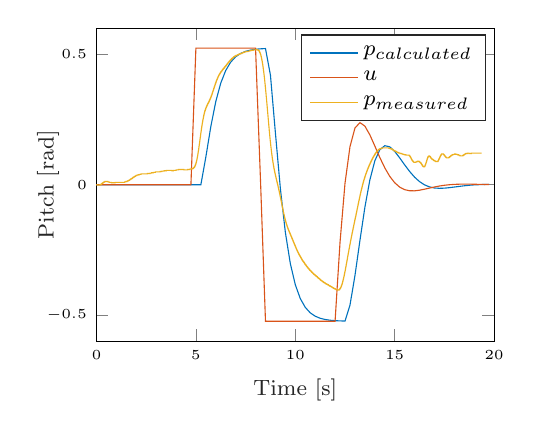
\begin{tikzpicture}

\begin{axis}[%
width=5.05cm,
height=3.975cm,
at={(0cm,0cm)},
scale only axis,
xmin=0,
xmax=20,
xlabel style={font=\color{white!15!black}},
xlabel={\footnotesize{Time [s]}},
ymin=-0.6,
ymax=0.6,
ylabel style={font=\color{white!15!black}},
ylabel={\footnotesize{Pitch [rad]}},
ylabel shift = -0.4cm,
ticklabel style = {font = \tiny},
axis background/.style={fill=white},
legend style={legend cell align=left, align=left, draw=white!15!black, font = \footnotesize}
]
\addplot [color=mycolor1]
  table[row sep=crcr]{%
0	0\\
5.25	0\\
5.5	0.106028752038569\\
5.75	0.222660379253369\\
6	0.318881471686371\\
6.25	0.389443606116966\\
6.5	0.437955073521682\\
6.75	0.469972641988527\\
7	0.490517248384048\\
7.25	0.503431000910158\\
7.5	0.511421385186051\\
7.75	0.516304397719924\\
8	0.519258620209424\\
8.25	0.521031153831515\\
8.5	0.522087287416479\\
8.75	0.419788185319383\\
9	0.197806850848963\\
9.25	-0.0154271414159268\\
9.5	-0.182835179527991\\
9.75	-0.302480738926231\\
10	-0.383449922872153\\
10.25	-0.43632324362575\\
10.5	-0.469990718255307\\
10.75	-0.491030760242825\\
11	-0.503990394682489\\
11.25	-0.511881380960279\\
11.5	-0.516641176643713\\
11.75	-0.519489919868132\\
12	-0.521183707800677\\
12.5	-0.522774229871597\\
12.75	-0.461630104891078\\
13	-0.348455686526812\\
13.25	-0.214121110126261\\
13.5	-0.0861143451593378\\
13.75	0.0182698683612337\\
14	0.0916543695165934\\
14.25	0.133995481406128\\
14.5	0.149716620167517\\
14.75	0.145321761536124\\
15	0.127687804335956\\
15.25	0.102998213212917\\
15.5	0.076194112189377\\
15.75	0.0508010642066203\\
16	0.0290016720803372\\
16.25	0.011847644417287\\
16.5	-0.00046875387968015\\
16.75	-0.00833924660917518\\
17	-0.0124943947394911\\
17.25	-0.0138063966993123\\
17.5	-0.0131452767335531\\
17.75	-0.0112857217577123\\
18.5	-0.00400621583755267\\
18.75	-0.00207432514593719\\
19	-0.000603273412565386\\
19.5	0.00101907497321108\\
19.75	0.00130023772636534\\
};
\addlegendentry{$p_{\text{calculated}}$}

\addplot [color=mycolor2]
  table[row sep=crcr]{%
0	0\\
4.75	0\\
5	0.523598775489244\\
8	0.523598769457593\\
8.25	0.0153288552853894\\
8.5	-0.523598758315433\\
12	-0.523598773540144\\
12.25	-0.219947793768711\\
12.5	0.00591715712205598\\
12.75	0.145861917647821\\
13	0.217338423729309\\
13.25	0.238143270238591\\
13.5	0.224730493375485\\
13.75	0.191122519097021\\
14	0.148380431602696\\
14.25	0.104528950504744\\
14.5	0.0648056506019365\\
14.75	0.0321059817681082\\
15	0.00751426403356703\\
15.25	-0.00916296150513318\\
15.5	-0.0189174301711397\\
15.75	-0.0231450515979361\\
16	-0.0233489231328114\\
16.25	-0.0209368143471487\\
16.5	-0.0171013408296368\\
17	-0.00858170258274882\\
17.25	-0.00494988815972874\\
17.5	-0.00207005308662644\\
17.75	1.13878316732041e-05\\
18	0.00135151349907048\\
18.25	0.00206788167972149\\
18.75	0.00220544735689998\\
19.75	0.00068557917430212\\
};
\addlegendentry{$u$}

\addplot [color=mycolor3]
  table[row sep=crcr]{%
0	0\\
0.032	0\\
0.0339999999999989	-0.00153398078788669\\
0.167999999999999	-0.00153398078788669\\
0.170000000000002	0\\
0.212	0\\
0.213999999999999	0.00153398078788669\\
0.248000000000001	0.00153398078788669\\
0.25	0.00306796157576983\\
0.27	0.00306796157576983\\
0.271999999999998	0.00460194236365652\\
0.297999999999998	0.00460194236365652\\
0.300000000000001	0.00613592315154321\\
0.315999999999999	0.00613592315154321\\
0.318000000000001	0.0076699039394299\\
0.346	0.0076699039394299\\
0.347999999999999	0.00920388472731304\\
0.373999999999999	0.00920388472731304\\
0.376000000000001	0.0107378655151997\\
0.379999999999999	0.0107378655151997\\
0.382000000000001	0.00920388472731304\\
0.384	0.00920388472731304\\
0.385999999999999	0.0107378655151997\\
0.416	0.0107378655151997\\
0.417999999999999	0.0122718463030864\\
0.422000000000001	0.0122718463030864\\
0.423999999999999	0.0107378655151997\\
0.425999999999998	0.0107378655151997\\
0.428000000000001	0.0122718463030864\\
0.568000000000001	0.0122718463030864\\
0.57	0.0107378655151997\\
0.634	0.0107378655151997\\
0.635999999999999	0.00920388472731304\\
0.744	0.00920388472731304\\
0.745999999999999	0.0076699039394299\\
0.936	0.0076699039394299\\
0.937999999999999	0.00920388472731304\\
1.412	0.00920388472731304\\
1.414	0.0107378655151997\\
1.48	0.0107378655151997\\
1.482	0.0122718463030864\\
1.536	0.0122718463030864\\
1.538	0.0138058270909696\\
1.578	0.0138058270909696\\
1.58	0.0153398078788562\\
1.616	0.0153398078788562\\
1.618	0.0168737886667429\\
1.654	0.0168737886667429\\
1.656	0.0184077694546261\\
1.692	0.0184077694546261\\
1.694	0.0199417502425128\\
1.716	0.0199417502425128\\
1.718	0.0214757310303995\\
1.742	0.0214757310303995\\
1.744	0.0230097118182861\\
1.774	0.0230097118182861\\
1.776	0.0245436926061693\\
1.8	0.0245436926061693\\
1.802	0.026077673394056\\
1.834	0.026077673394056\\
1.836	0.0276116541819427\\
1.86	0.0276116541819427\\
1.862	0.0291456349698258\\
1.892	0.0291456349698258\\
1.894	0.0306796157577125\\
1.92	0.0306796157577125\\
1.922	0.0322135965455992\\
1.958	0.0322135965455992\\
1.96	0.0337475773334859\\
1.998	0.0337475773334859\\
2	0.035281558121369\\
2.036	0.035281558121369\\
2.038	0.0368155389092557\\
2.094	0.0368155389092557\\
2.096	0.0383495196971424\\
2.16	0.0383495196971424\\
2.162	0.0398835004850255\\
2.238	0.0398835004850255\\
2.24	0.0414174812729122\\
2.558	0.0414174812729122\\
2.56	0.0429514620607989\\
2.694	0.0429514620607989\\
2.696	0.0444854428486821\\
2.772	0.0444854428486821\\
2.774	0.0460194236365687\\
2.856	0.0460194236365687\\
2.858	0.0475534044244554\\
2.956	0.0475534044244554\\
2.958	0.0490873852123421\\
3.196	0.0490873852123421\\
3.198	0.0506213660002253\\
3.288	0.0506213660002253\\
3.29	0.052155346788112\\
3.406	0.052155346788112\\
3.408	0.0536893275759986\\
3.512	0.0536893275759986\\
3.514	0.0552233083638818\\
3.788	0.0552233083638818\\
3.79	0.0536893275759986\\
3.872	0.0536893275759986\\
3.874	0.0552233083638818\\
4.004	0.0552233083638818\\
4.006	0.0567572891517685\\
4.12	0.0567572891517685\\
4.122	0.0582912699396552\\
4.39	0.0582912699396552\\
4.392	0.0567572891517685\\
4.578	0.0567572891517685\\
4.58	0.0582912699396552\\
4.678	0.0582912699396552\\
4.68	0.0598252507275383\\
4.766	0.0598252507275383\\
4.768	0.061359231515425\\
4.844	0.061359231515425\\
4.846	0.0628932123033117\\
4.876	0.0628932123033117\\
4.878	0.0644271930911984\\
4.902	0.0644271930911984\\
4.904	0.0659611738790815\\
4.916	0.0659611738790815\\
4.918	0.0674951546669682\\
4.93	0.0674951546669682\\
4.932	0.0690291354548549\\
4.942	0.0690291354548549\\
4.944	0.070563116242738\\
4.952	0.070563116242738\\
4.954	0.0720970970306247\\
4.96	0.0720970970306247\\
4.962	0.0736310778185114\\
4.97	0.0736310778185114\\
4.972	0.0751650586063981\\
4.978	0.0751650586063981\\
4.98	0.0766990393942812\\
4.984	0.0766990393942812\\
4.986	0.0782330201821679\\
4.992	0.0782330201821679\\
4.994	0.0797670009700546\\
4.998	0.0797670009700546\\
5	0.0813009817579378\\
5.004	0.0813009817579378\\
5.006	0.0828349625458245\\
5.01	0.0828349625458245\\
5.012	0.0843689433337111\\
5.016	0.0843689433337111\\
5.018	0.0859029241215943\\
5.02	0.0859029241215943\\
5.022	0.087436904909481\\
5.024	0.087436904909481\\
5.026	0.0889708856973677\\
5.03	0.0889708856973677\\
5.032	0.0905048664852544\\
5.034	0.0905048664852544\\
5.036	0.0920388472731375\\
5.04	0.0920388472731375\\
5.042	0.0935728280610242\\
5.044	0.0935728280610242\\
5.046	0.0951068088489109\\
5.048	0.0951068088489109\\
5.05	0.096640789636794\\
5.052	0.096640789636794\\
5.054	0.0981747704246807\\
5.056	0.0981747704246807\\
5.058	0.0997087512125674\\
5.06	0.0997087512125674\\
5.062	0.101242732000454\\
5.064	0.101242732000454\\
5.066	0.102776712788337\\
5.068	0.102776712788337\\
5.07	0.104310693576224\\
5.072	0.104310693576224\\
5.074	0.105844674364111\\
5.076	0.105844674364111\\
5.078	0.107378655151994\\
5.08	0.107378655151994\\
5.084	0.110446616727767\\
5.086	0.110446616727767\\
5.088	0.11198059751565\\
5.09	0.11198059751565\\
5.092	0.113514578303537\\
5.094	0.113514578303537\\
5.098	0.11658253987931\\
5.1	0.11658253987931\\
5.102	0.118116520667193\\
5.104	0.118116520667193\\
5.108	0.121184482242967\\
5.11	0.121184482242967\\
5.112	0.12271846303085\\
5.114	0.12271846303085\\
5.118	0.125786424606623\\
5.12	0.125786424606623\\
5.124	0.128854386182393\\
5.126	0.128854386182393\\
5.13	0.131922347758167\\
5.132	0.131922347758167\\
5.136	0.134990309333936\\
5.138	0.134990309333936\\
5.142	0.138058270909706\\
5.144	0.138058270909706\\
5.148	0.14112623248548\\
5.15	0.14112623248548\\
5.156	0.145728174849136\\
5.158	0.145728174849136\\
5.162	0.148796136424906\\
5.164	0.148796136424906\\
5.17	0.153398078788562\\
5.172	0.153398078788562\\
5.176	0.156466040364336\\
5.178	0.156466040364336\\
5.184	0.161067982727992\\
5.186	0.161067982727992\\
5.19	0.164135944303762\\
5.192	0.164135944303762\\
5.198	0.168737886667422\\
5.2	0.168737886667422\\
5.206	0.173339829031079\\
5.208	0.173339829031079\\
5.214	0.177941771394735\\
5.216	0.177941771394735\\
5.222	0.182543713758392\\
5.224	0.182543713758392\\
5.228	0.185611675334162\\
5.23	0.185611675334162\\
5.236	0.190213617697818\\
5.238	0.190213617697818\\
5.244	0.194815560061475\\
5.246	0.194815560061475\\
5.252	0.199417502425135\\
5.254	0.199417502425135\\
5.258	0.202485464000905\\
5.26	0.202485464000905\\
5.264	0.205553425576674\\
5.266	0.205553425576674\\
5.272	0.210155367940335\\
5.274	0.210155367940335\\
5.278	0.213223329516104\\
5.28	0.213223329516104\\
5.284	0.216291291091874\\
5.286	0.216291291091874\\
5.29	0.219359252667648\\
5.292	0.219359252667648\\
5.296	0.222427214243417\\
5.298	0.222427214243417\\
5.302	0.225495175819191\\
5.304	0.225495175819191\\
5.306	0.227029156607074\\
5.308	0.227029156607074\\
5.312	0.230097118182847\\
5.314	0.230097118182847\\
5.318	0.233165079758617\\
5.32	0.233165079758617\\
5.322	0.234699060546504\\
5.324	0.234699060546504\\
5.328	0.237767022122274\\
5.33	0.237767022122274\\
5.332	0.23930100291016\\
5.334	0.23930100291016\\
5.338	0.24236896448593\\
5.34	0.24236896448593\\
5.342	0.243902945273817\\
5.344	0.243902945273817\\
5.348	0.246970906849587\\
5.35	0.246970906849587\\
5.352	0.248504887637473\\
5.356	0.248504887637473\\
5.36	0.251572849213247\\
5.362	0.251572849213247\\
5.364	0.25310683000113\\
5.366	0.25310683000113\\
5.368	0.254640810789017\\
5.37	0.254640810789017\\
5.372	0.256174791576903\\
5.374	0.256174791576903\\
5.376	0.257708772364786\\
5.378	0.257708772364786\\
5.38	0.259242753152673\\
5.382	0.259242753152673\\
5.384	0.26077673394056\\
5.386	0.26077673394056\\
5.388	0.262310714728443\\
5.39	0.262310714728443\\
5.392	0.26384469551633\\
5.394	0.26384469551633\\
5.396	0.265378676304216\\
5.4	0.265378676304216\\
5.402	0.266912657092103\\
5.404	0.266912657092103\\
5.406	0.268446637879986\\
5.408	0.268446637879986\\
5.41	0.269980618667873\\
5.412	0.269980618667873\\
5.414	0.27151459945576\\
5.418	0.27151459945576\\
5.42	0.273048580243643\\
5.422	0.273048580243643\\
5.424	0.274582561031529\\
5.428	0.274582561031529\\
5.43	0.276116541819416\\
5.434	0.276116541819416\\
5.436	0.277650522607303\\
5.438	0.277650522607303\\
5.44	0.279184503395186\\
5.442	0.279184503395186\\
5.444	0.280718484183073\\
5.45	0.280718484183073\\
5.452	0.282252464970959\\
5.456	0.282252464970959\\
5.458	0.283786445758842\\
5.462	0.283786445758842\\
5.464	0.285320426546729\\
5.47	0.285320426546729\\
5.472	0.286854407334616\\
5.474	0.286854407334616\\
5.476	0.288388388122499\\
5.482	0.288388388122499\\
5.484	0.289922368910386\\
5.488	0.289922368910386\\
5.49	0.291456349698272\\
5.496	0.291456349698272\\
5.498	0.292990330486159\\
5.504	0.292990330486159\\
5.506	0.294524311274042\\
5.512	0.294524311274042\\
5.514	0.296058292061929\\
5.52	0.296058292061929\\
5.522	0.297592272849815\\
5.528	0.297592272849815\\
5.53	0.299126253637699\\
5.536	0.299126253637699\\
5.538	0.300660234425585\\
5.546	0.300660234425585\\
5.548	0.302194215213472\\
5.554	0.302194215213472\\
5.556	0.303728196001359\\
5.564	0.303728196001359\\
5.566	0.305262176789242\\
5.576	0.305262176789242\\
5.578	0.306796157577129\\
5.584	0.306796157577129\\
5.586	0.308330138365015\\
5.594	0.308330138365015\\
5.596	0.309864119152898\\
5.606	0.309864119152898\\
5.608	0.311398099940785\\
5.616	0.311398099940785\\
5.618	0.312932080728672\\
5.626	0.312932080728672\\
5.628	0.314466061516555\\
5.636	0.314466061516555\\
5.638	0.316000042304442\\
5.648	0.316000042304442\\
5.65	0.317534023092328\\
5.654	0.317534023092328\\
5.656	0.319068003880215\\
5.664	0.319068003880215\\
5.666	0.320601984668098\\
5.676	0.320601984668098\\
5.678	0.322135965455985\\
5.682	0.322135965455985\\
5.684	0.323669946243871\\
5.692	0.323669946243871\\
5.694	0.325203927031755\\
5.702	0.325203927031755\\
5.704	0.326737907819641\\
5.71	0.326737907819641\\
5.712	0.328271888607528\\
5.72	0.328271888607528\\
5.722	0.329805869395411\\
5.726	0.329805869395411\\
5.728	0.331339850183298\\
5.736	0.331339850183298\\
5.738	0.332873830971185\\
5.744	0.332873830971185\\
5.746	0.334407811759071\\
5.752	0.334407811759071\\
5.754	0.335941792546954\\
5.76	0.335941792546954\\
5.762	0.337475773334841\\
5.768	0.337475773334841\\
5.77	0.339009754122728\\
5.774	0.339009754122728\\
5.776	0.340543734910611\\
5.782	0.340543734910611\\
5.784	0.342077715698498\\
5.79	0.342077715698498\\
5.792	0.343611696486384\\
5.798	0.343611696486384\\
5.8	0.345145677274271\\
5.804	0.345145677274271\\
5.806	0.346679658062154\\
5.812	0.346679658062154\\
5.814	0.348213638850041\\
5.818	0.348213638850041\\
5.82	0.349747619637927\\
5.824	0.349747619637927\\
5.826	0.351281600425811\\
5.832	0.351281600425811\\
5.834	0.352815581213697\\
5.838	0.352815581213697\\
5.84	0.354349562001584\\
5.844	0.354349562001584\\
5.846	0.355883542789467\\
5.852	0.355883542789467\\
5.854	0.357417523577354\\
5.858	0.357417523577354\\
5.86	0.35895150436524\\
5.864	0.35895150436524\\
5.866	0.360485485153127\\
5.872	0.360485485153127\\
5.874	0.36201946594101\\
5.878	0.36201946594101\\
5.88	0.363553446728897\\
5.886	0.363553446728897\\
5.888	0.365087427516784\\
5.89	0.365087427516784\\
5.892	0.366621408304667\\
5.896	0.366621408304667\\
5.898	0.368155389092554\\
5.904	0.368155389092554\\
5.906	0.36968936988044\\
5.91	0.36968936988044\\
5.912	0.371223350668327\\
5.918	0.371223350668327\\
5.92	0.37275733145621\\
5.922	0.37275733145621\\
5.924	0.374291312244097\\
5.93	0.374291312244097\\
5.932	0.375825293031983\\
5.936	0.375825293031983\\
5.938	0.377359273819867\\
5.944	0.377359273819867\\
5.946	0.378893254607753\\
5.948	0.378893254607753\\
5.95	0.38042723539564\\
5.956	0.38042723539564\\
5.958	0.381961216183523\\
5.962	0.381961216183523\\
5.964	0.38349519697141\\
5.97	0.38349519697141\\
5.972	0.385029177759296\\
5.976	0.385029177759296\\
5.978	0.386563158547183\\
5.984	0.386563158547183\\
5.986	0.388097139335066\\
5.99	0.388097139335066\\
5.992	0.389631120122953\\
5.998	0.389631120122953\\
6	0.39116510091084\\
6.004	0.39116510091084\\
6.006	0.392699081698723\\
6.012	0.392699081698723\\
6.014	0.394233062486609\\
6.02	0.394233062486609\\
6.022	0.395767043274496\\
6.028	0.395767043274496\\
6.03	0.397301024062379\\
6.034	0.397301024062379\\
6.036	0.398835004850266\\
6.042	0.398835004850266\\
6.044	0.400368985638153\\
6.048	0.400368985638153\\
6.05	0.401902966426039\\
6.058	0.401902966426039\\
6.06	0.403436947213923\\
6.064	0.403436947213923\\
6.066	0.404970928001809\\
6.076	0.404970928001809\\
6.078	0.406504908789696\\
6.082	0.406504908789696\\
6.084	0.408038889577579\\
6.092	0.408038889577579\\
6.094	0.409572870365466\\
6.102	0.409572870365466\\
6.104	0.411106851153352\\
6.11	0.411106851153352\\
6.112	0.412640831941239\\
6.12	0.412640831941239\\
6.122	0.414174812729122\\
6.13	0.414174812729122\\
6.132	0.415708793517009\\
6.136	0.415708793517009\\
6.138	0.417242774304896\\
6.148	0.417242774304896\\
6.15	0.418776755092779\\
6.16	0.418776755092779\\
6.162	0.420310735880665\\
6.172	0.420310735880665\\
6.174	0.421844716668552\\
6.18	0.421844716668552\\
6.182	0.423378697456435\\
6.194	0.423378697456435\\
6.196	0.424912678244322\\
6.206	0.424912678244322\\
6.208	0.426446659032209\\
6.22	0.426446659032209\\
6.222	0.427980639820095\\
6.232	0.427980639820095\\
6.234	0.429514620607979\\
6.246	0.429514620607979\\
6.248	0.431048601395865\\
6.258	0.431048601395865\\
6.26	0.432582582183752\\
6.272	0.432582582183752\\
6.274	0.434116562971635\\
6.288	0.434116562971635\\
6.29	0.435650543759522\\
6.302	0.435650543759522\\
6.304	0.437184524547408\\
6.318	0.437184524547408\\
6.32	0.438718505335295\\
6.334	0.438718505335295\\
6.336	0.440252486123178\\
6.348	0.440252486123178\\
6.35	0.441786466911065\\
6.362	0.441786466911065\\
6.364	0.443320447698952\\
6.38	0.443320447698952\\
6.382	0.444854428486835\\
6.396	0.444854428486835\\
6.398	0.446388409274721\\
6.414	0.446388409274721\\
6.416	0.447922390062608\\
6.432	0.447922390062608\\
6.434	0.449456370850491\\
6.446	0.449456370850491\\
6.448	0.450990351638378\\
6.462	0.450990351638378\\
6.464	0.452524332426265\\
6.478	0.452524332426265\\
6.48	0.454058313214151\\
6.494	0.454058313214151\\
6.496	0.455592294002034\\
6.51	0.455592294002034\\
6.512	0.457126274789921\\
6.528	0.457126274789921\\
6.53	0.458660255577808\\
6.542	0.458660255577808\\
6.544	0.460194236365691\\
6.56	0.460194236365691\\
6.562	0.461728217153578\\
6.574	0.461728217153578\\
6.576	0.463262197941464\\
6.59	0.463262197941464\\
6.592	0.464796178729351\\
6.606	0.464796178729351\\
6.608	0.466330159517234\\
6.62	0.466330159517234\\
6.622	0.467864140305121\\
6.636	0.467864140305121\\
6.638	0.469398121093008\\
6.654	0.469398121093008\\
6.656	0.470932101880891\\
6.67	0.470932101880891\\
6.672	0.472466082668777\\
6.688	0.472466082668777\\
6.69	0.474000063456664\\
6.706	0.474000063456664\\
6.708	0.475534044244547\\
6.724	0.475534044244547\\
6.726	0.477068025032434\\
6.74	0.477068025032434\\
6.742	0.478602005820321\\
6.758	0.478602005820321\\
6.76	0.480135986608207\\
6.782	0.480135986608207\\
6.784	0.48166996739609\\
6.8	0.48166996739609\\
6.802	0.483203948183977\\
6.824	0.483203948183977\\
6.826	0.484737928971864\\
6.842	0.484737928971864\\
6.844	0.486271909759747\\
6.87	0.486271909759747\\
6.872	0.487805890547634\\
6.896	0.487805890547634\\
6.898	0.48933987133552\\
6.914	0.48933987133552\\
6.916	0.490873852123404\\
6.942	0.490873852123404\\
6.944	0.49240783291129\\
6.982	0.49240783291129\\
6.984	0.493941813699177\\
7.014	0.493941813699177\\
7.016	0.495475794487064\\
7.054	0.495475794487064\\
7.056	0.497009775274947\\
7.104	0.497009775274947\\
7.106	0.498543756062833\\
7.148	0.498543756062833\\
7.15	0.50007773685072\\
7.202	0.50007773685072\\
7.204	0.501611717638603\\
7.246	0.501611717638603\\
7.248	0.50314569842649\\
7.3	0.50314569842649\\
7.302	0.504679679214377\\
7.352	0.504679679214377\\
7.354	0.506213660002263\\
7.398	0.506213660002263\\
7.4	0.507747640790146\\
7.452	0.507747640790146\\
7.454	0.509281621578033\\
7.512	0.509281621578033\\
7.514	0.51081560236592\\
7.62	0.51081560236592\\
7.622	0.512349583153803\\
7.718	0.512349583153803\\
7.72	0.51388356394169\\
7.784	0.51388356394169\\
7.786	0.515417544729576\\
7.87	0.515417544729576\\
7.872	0.516951525517459\\
7.876	0.516951525517459\\
7.878	0.515417544729576\\
7.884	0.515417544729576\\
7.886	0.516951525517459\\
8.036	0.516951525517459\\
8.038	0.518485506305346\\
8.072	0.518485506305346\\
8.074	0.516951525517459\\
8.08	0.516951525517459\\
8.082	0.518485506305346\\
8.084	0.518485506305346\\
8.086	0.516951525517459\\
8.132	0.516951525517459\\
8.134	0.515417544729576\\
8.158	0.515417544729576\\
8.16	0.51388356394169\\
8.174	0.51388356394169\\
8.176	0.512349583153803\\
8.188	0.512349583153803\\
8.19	0.51081560236592\\
8.2	0.51081560236592\\
8.202	0.509281621578033\\
8.21	0.509281621578033\\
8.212	0.507747640790146\\
8.218	0.507747640790146\\
8.22	0.506213660002263\\
8.228	0.506213660002263\\
8.23	0.504679679214377\\
8.234	0.504679679214377\\
8.236	0.50314569842649\\
8.242	0.50314569842649\\
8.244	0.501611717638603\\
8.248	0.501611717638603\\
8.25	0.50007773685072\\
8.254	0.50007773685072\\
8.256	0.498543756062833\\
8.262	0.498543756062833\\
8.264	0.497009775274947\\
8.266	0.497009775274947\\
8.268	0.495475794487064\\
8.272	0.495475794487064\\
8.274	0.493941813699177\\
8.278	0.493941813699177\\
8.28	0.49240783291129\\
8.282	0.49240783291129\\
8.284	0.490873852123404\\
8.288	0.490873852123404\\
8.29	0.48933987133552\\
8.292	0.48933987133552\\
8.294	0.487805890547634\\
8.296	0.487805890547634\\
8.298	0.486271909759747\\
8.3	0.486271909759747\\
8.302	0.484737928971864\\
8.306	0.484737928971864\\
8.308	0.483203948183977\\
8.31	0.483203948183977\\
8.312	0.48166996739609\\
8.314	0.48166996739609\\
8.316	0.480135986608207\\
8.318	0.480135986608207\\
8.32	0.478602005820321\\
8.322	0.478602005820321\\
8.324	0.477068025032434\\
8.326	0.477068025032434\\
8.33	0.474000063456664\\
8.332	0.474000063456664\\
8.334	0.472466082668777\\
8.336	0.472466082668777\\
8.338	0.470932101880891\\
8.34	0.470932101880891\\
8.344	0.467864140305121\\
8.346	0.467864140305121\\
8.348	0.466330159517234\\
8.35	0.466330159517234\\
8.354	0.463262197941464\\
8.356	0.463262197941464\\
8.36	0.460194236365691\\
8.362	0.460194236365691\\
8.366	0.457126274789921\\
8.368	0.457126274789921\\
8.37	0.455592294002034\\
8.372	0.455592294002034\\
8.378	0.450990351638378\\
8.38	0.450990351638378\\
8.384	0.447922390062608\\
8.386	0.447922390062608\\
8.392	0.443320447698952\\
8.394	0.443320447698952\\
8.4	0.438718505335295\\
8.402	0.438718505335295\\
8.41	0.432582582183752\\
8.412	0.432582582183752\\
8.418	0.427980639820095\\
8.42	0.427980639820095\\
8.432	0.418776755092779\\
8.434	0.418776755092779\\
8.448	0.408038889577579\\
8.45	0.408038889577579\\
8.482	0.38349519697141\\
8.484	0.38349519697141\\
8.488	0.38042723539564\\
8.49	0.377359273819867\\
8.498	0.371223350668327\\
8.5	0.371223350668327\\
8.502	0.36968936988044\\
8.504	0.366621408304667\\
8.534	0.343611696486384\\
8.536	0.340543734910611\\
8.554	0.326737907819641\\
8.556	0.323669946243871\\
8.574	0.309864119152898\\
8.576	0.306796157577129\\
8.588	0.297592272849815\\
8.59	0.294524311274042\\
8.6	0.286854407334616\\
8.602	0.283786445758842\\
8.616	0.273048580243643\\
8.618	0.269980618667873\\
8.63	0.26077673394056\\
8.632	0.257708772364786\\
8.644	0.248504887637473\\
8.646	0.245436926061704\\
8.662	0.233165079758617\\
8.664	0.230097118182847\\
8.68	0.217825271879761\\
8.682	0.214757310303991\\
8.708	0.194815560061475\\
8.71	0.191747598485705\\
8.744	0.165669925091649\\
8.746	0.165669925091649\\
8.748	0.162601963515879\\
8.75	0.162601963515879\\
8.77	0.147262155637023\\
8.772	0.147262155637023\\
8.788	0.134990309333936\\
8.79	0.134990309333936\\
8.798	0.128854386182393\\
8.8	0.128854386182393\\
8.808	0.12271846303085\\
8.81	0.12271846303085\\
8.818	0.11658253987931\\
8.82	0.11658253987931\\
8.826	0.11198059751565\\
8.828	0.11198059751565\\
8.834	0.107378655151994\\
8.836	0.107378655151994\\
8.84	0.104310693576224\\
8.842	0.104310693576224\\
8.846	0.101242732000454\\
8.848	0.101242732000454\\
8.854	0.096640789636794\\
8.856	0.096640789636794\\
8.86	0.0935728280610242\\
8.862	0.0935728280610242\\
8.864	0.0920388472731375\\
8.866	0.0920388472731375\\
8.872	0.087436904909481\\
8.874	0.087436904909481\\
8.876	0.0859029241215943\\
8.878	0.0859029241215943\\
8.882	0.0828349625458245\\
8.884	0.0828349625458245\\
8.886	0.0813009817579378\\
8.888	0.0813009817579378\\
8.89	0.0797670009700546\\
8.892	0.0797670009700546\\
8.896	0.0766990393942812\\
8.898	0.0766990393942812\\
8.902	0.0736310778185114\\
8.904	0.0736310778185114\\
8.906	0.0720970970306247\\
8.908	0.0720970970306247\\
8.91	0.070563116242738\\
8.912	0.070563116242738\\
8.914	0.0690291354548549\\
8.916	0.0690291354548549\\
8.918	0.0674951546669682\\
8.92	0.0674951546669682\\
8.924	0.0644271930911984\\
8.926	0.0644271930911984\\
8.928	0.0628932123033117\\
8.93	0.0628932123033117\\
8.932	0.061359231515425\\
8.934	0.061359231515425\\
8.936	0.0598252507275383\\
8.938	0.0598252507275383\\
8.94	0.0582912699396552\\
8.942	0.0582912699396552\\
8.944	0.0567572891517685\\
8.946	0.0567572891517685\\
8.948	0.0552233083638818\\
8.95	0.0552233083638818\\
8.952	0.0536893275759986\\
8.954	0.0536893275759986\\
8.956	0.052155346788112\\
8.96	0.052155346788112\\
8.964	0.0490873852123421\\
8.966	0.0490873852123421\\
8.968	0.0475534044244554\\
8.972	0.0475534044244554\\
8.974	0.0460194236365687\\
8.976	0.0460194236365687\\
8.978	0.0444854428486821\\
8.98	0.0444854428486821\\
8.982	0.0429514620607989\\
8.984	0.0429514620607989\\
8.986	0.0414174812729122\\
8.99	0.0414174812729122\\
8.992	0.0398835004850255\\
8.994	0.0398835004850255\\
8.996	0.0383495196971424\\
8.998	0.0383495196971424\\
9	0.0368155389092557\\
9.002	0.0368155389092557\\
9.004	0.035281558121369\\
9.006	0.035281558121369\\
9.008	0.0337475773334859\\
9.012	0.0337475773334859\\
9.014	0.0322135965455992\\
9.016	0.0322135965455992\\
9.018	0.0306796157577125\\
9.022	0.0306796157577125\\
9.024	0.0291456349698258\\
9.026	0.0291456349698258\\
9.028	0.0276116541819427\\
9.03	0.0276116541819427\\
9.032	0.026077673394056\\
9.034	0.026077673394056\\
9.036	0.0245436926061693\\
9.04	0.0245436926061693\\
9.042	0.0230097118182861\\
9.044	0.0230097118182861\\
9.046	0.0214757310303995\\
9.05	0.0214757310303995\\
9.052	0.0199417502425128\\
9.054	0.0199417502425128\\
9.056	0.0184077694546261\\
9.058	0.0184077694546261\\
9.06	0.0168737886667429\\
9.064	0.0168737886667429\\
9.066	0.0153398078788562\\
9.068	0.0153398078788562\\
9.07	0.0138058270909696\\
9.074	0.0138058270909696\\
9.076	0.0122718463030864\\
9.078	0.0122718463030864\\
9.08	0.0107378655151997\\
9.082	0.0107378655151997\\
9.084	0.00920388472731304\\
9.088	0.00920388472731304\\
9.09	0.0076699039394299\\
9.092	0.0076699039394299\\
9.094	0.00613592315154321\\
9.096	0.00613592315154321\\
9.098	0.00460194236365652\\
9.102	0.00460194236365652\\
9.104	0.00306796157576983\\
9.106	0.00306796157576983\\
9.108	0.00153398078788669\\
9.112	0.00153398078788669\\
9.114	0\\
9.116	0\\
9.118	-0.00153398078788669\\
9.12	-0.00153398078788669\\
9.122	-0.00306796157576983\\
9.126	-0.00306796157576983\\
9.128	-0.00460194236365652\\
9.13	-0.00460194236365652\\
9.132	-0.00613592315154321\\
9.134	-0.00613592315154321\\
9.136	-0.0076699039394299\\
9.14	-0.0076699039394299\\
9.142	-0.00920388472731304\\
9.144	-0.00920388472731304\\
9.146	-0.0107378655151997\\
9.148	-0.0107378655151997\\
9.15	-0.0122718463030864\\
9.154	-0.0122718463030864\\
9.156	-0.0138058270909696\\
9.158	-0.0138058270909696\\
9.16	-0.0153398078788562\\
9.162	-0.0153398078788562\\
9.164	-0.0168737886667429\\
9.166	-0.0168737886667429\\
9.168	-0.0184077694546261\\
9.172	-0.0184077694546261\\
9.174	-0.0199417502425128\\
9.176	-0.0199417502425128\\
9.178	-0.0214757310303995\\
9.18	-0.0214757310303995\\
9.182	-0.0230097118182861\\
9.184	-0.0230097118182861\\
9.186	-0.0245436926061693\\
9.188	-0.0245436926061693\\
9.19	-0.026077673394056\\
9.194	-0.026077673394056\\
9.196	-0.0276116541819427\\
9.198	-0.0276116541819427\\
9.2	-0.0291456349698258\\
9.202	-0.0291456349698258\\
9.204	-0.0306796157577125\\
9.206	-0.0306796157577125\\
9.208	-0.0322135965455992\\
9.21	-0.0322135965455992\\
9.212	-0.0337475773334859\\
9.214	-0.0337475773334859\\
9.216	-0.035281558121369\\
9.218	-0.035281558121369\\
9.22	-0.0368155389092557\\
9.224	-0.0368155389092557\\
9.226	-0.0383495196971424\\
9.228	-0.0383495196971424\\
9.23	-0.0398835004850255\\
9.232	-0.0398835004850255\\
9.234	-0.0414174812729122\\
9.236	-0.0414174812729122\\
9.238	-0.0429514620607989\\
9.24	-0.0429514620607989\\
9.242	-0.0444854428486821\\
9.244	-0.0444854428486821\\
9.246	-0.0460194236365687\\
9.248	-0.0460194236365687\\
9.25	-0.0475534044244554\\
9.252	-0.0475534044244554\\
9.254	-0.0490873852123421\\
9.256	-0.0490873852123421\\
9.258	-0.0506213660002253\\
9.26	-0.0506213660002253\\
9.262	-0.052155346788112\\
9.264	-0.052155346788112\\
9.266	-0.0536893275759986\\
9.268	-0.0536893275759986\\
9.27	-0.0552233083638818\\
9.272	-0.0552233083638818\\
9.274	-0.0567572891517685\\
9.276	-0.0567572891517685\\
9.278	-0.0582912699396552\\
9.28	-0.0582912699396552\\
9.282	-0.0598252507275383\\
9.284	-0.0598252507275383\\
9.286	-0.061359231515425\\
9.29	-0.061359231515425\\
9.292	-0.0628932123033117\\
9.294	-0.0628932123033117\\
9.296	-0.0644271930911984\\
9.298	-0.0644271930911984\\
9.3	-0.0659611738790815\\
9.302	-0.0659611738790815\\
9.304	-0.0674951546669682\\
9.306	-0.0674951546669682\\
9.308	-0.0690291354548549\\
9.31	-0.0690291354548549\\
9.312	-0.070563116242738\\
9.314	-0.070563116242738\\
9.316	-0.0720970970306247\\
9.318	-0.0720970970306247\\
9.32	-0.0736310778185114\\
9.322	-0.0736310778185114\\
9.324	-0.0751650586063981\\
9.326	-0.0751650586063981\\
9.328	-0.0766990393942812\\
9.33	-0.0766990393942812\\
9.332	-0.0782330201821679\\
9.334	-0.0782330201821679\\
9.336	-0.0797670009700546\\
9.338	-0.0797670009700546\\
9.34	-0.0813009817579378\\
9.342	-0.0813009817579378\\
9.344	-0.0828349625458245\\
9.346	-0.0828349625458245\\
9.348	-0.0843689433337111\\
9.35	-0.0843689433337111\\
9.352	-0.0859029241215943\\
9.354	-0.0859029241215943\\
9.356	-0.087436904909481\\
9.358	-0.087436904909481\\
9.36	-0.0889708856973677\\
9.362	-0.0889708856973677\\
9.364	-0.0905048664852544\\
9.366	-0.0905048664852544\\
9.368	-0.0920388472731375\\
9.37	-0.0920388472731375\\
9.372	-0.0935728280610242\\
9.374	-0.0935728280610242\\
9.376	-0.0951068088489109\\
9.378	-0.0951068088489109\\
9.38	-0.096640789636794\\
9.384	-0.096640789636794\\
9.386	-0.0981747704246807\\
9.388	-0.0981747704246807\\
9.39	-0.0997087512125674\\
9.392	-0.0997087512125674\\
9.394	-0.101242732000454\\
9.396	-0.101242732000454\\
9.398	-0.102776712788337\\
9.4	-0.102776712788337\\
9.402	-0.104310693576224\\
9.404	-0.104310693576224\\
9.406	-0.105844674364111\\
9.408	-0.105844674364111\\
9.41	-0.107378655151994\\
9.414	-0.107378655151994\\
9.416	-0.10891263593988\\
9.418	-0.10891263593988\\
9.42	-0.110446616727767\\
9.422	-0.110446616727767\\
9.424	-0.11198059751565\\
9.426	-0.11198059751565\\
9.428	-0.113514578303537\\
9.43	-0.113514578303537\\
9.432	-0.115048559091424\\
9.434	-0.115048559091424\\
9.436	-0.11658253987931\\
9.44	-0.11658253987931\\
9.442	-0.118116520667193\\
9.444	-0.118116520667193\\
9.446	-0.11965050145508\\
9.448	-0.11965050145508\\
9.45	-0.121184482242967\\
9.454	-0.121184482242967\\
9.456	-0.12271846303085\\
9.458	-0.12271846303085\\
9.46	-0.124252443818737\\
9.462	-0.124252443818737\\
9.464	-0.125786424606623\\
9.468	-0.125786424606623\\
9.47	-0.127320405394507\\
9.472	-0.127320405394507\\
9.474	-0.128854386182393\\
9.478	-0.128854386182393\\
9.48	-0.13038836697028\\
9.484	-0.13038836697028\\
9.486	-0.131922347758167\\
9.488	-0.131922347758167\\
9.49	-0.13345632854605\\
9.494	-0.13345632854605\\
9.496	-0.134990309333936\\
9.498	-0.134990309333936\\
9.5	-0.136524290121823\\
9.504	-0.136524290121823\\
9.506	-0.138058270909706\\
9.51	-0.138058270909706\\
9.512	-0.139592251697593\\
9.514	-0.139592251697593\\
9.516	-0.14112623248548\\
9.52	-0.14112623248548\\
9.522	-0.142660213273366\\
9.526	-0.142660213273366\\
9.528	-0.144194194061249\\
9.532	-0.144194194061249\\
9.534	-0.145728174849136\\
9.538	-0.145728174849136\\
9.54	-0.147262155637023\\
9.544	-0.147262155637023\\
9.546	-0.148796136424906\\
9.55	-0.148796136424906\\
9.552	-0.150330117212793\\
9.556	-0.150330117212793\\
9.558	-0.151864098000679\\
9.562	-0.151864098000679\\
9.564	-0.153398078788562\\
9.57	-0.153398078788562\\
9.572	-0.154932059576449\\
9.576	-0.154932059576449\\
9.578	-0.156466040364336\\
9.582	-0.156466040364336\\
9.584	-0.158000021152223\\
9.59	-0.158000021152223\\
9.592	-0.159534001940106\\
9.596	-0.159534001940106\\
9.598	-0.161067982727992\\
9.602	-0.161067982727992\\
9.604	-0.162601963515879\\
9.61	-0.162601963515879\\
9.612	-0.164135944303762\\
9.618	-0.164135944303762\\
9.62	-0.165669925091649\\
9.626	-0.165669925091649\\
9.628	-0.167203905879536\\
9.632	-0.167203905879536\\
9.634	-0.168737886667422\\
9.64	-0.168737886667422\\
9.642	-0.170271867455305\\
9.648	-0.170271867455305\\
9.65	-0.171805848243192\\
9.656	-0.171805848243192\\
9.658	-0.173339829031079\\
9.664	-0.173339829031079\\
9.666	-0.174873809818962\\
9.672	-0.174873809818962\\
9.674	-0.176407790606849\\
9.68	-0.176407790606849\\
9.682	-0.177941771394735\\
9.69	-0.177941771394735\\
9.692	-0.179475752182618\\
9.698	-0.179475752182618\\
9.7	-0.181009732970505\\
9.706	-0.181009732970505\\
9.708	-0.182543713758392\\
9.714	-0.182543713758392\\
9.716	-0.184077694546279\\
9.724	-0.184077694546279\\
9.726	-0.185611675334162\\
9.73	-0.185611675334162\\
9.732	-0.187145656122048\\
9.74	-0.187145656122048\\
9.742	-0.188679636909935\\
9.748	-0.188679636909935\\
9.75	-0.190213617697818\\
9.756	-0.190213617697818\\
9.758	-0.191747598485705\\
9.764	-0.191747598485705\\
9.766	-0.193281579273592\\
9.774	-0.193281579273592\\
9.776	-0.194815560061475\\
9.782	-0.194815560061475\\
9.784	-0.196349540849361\\
9.79	-0.196349540849361\\
9.792	-0.197883521637248\\
9.8	-0.197883521637248\\
9.802	-0.199417502425135\\
9.808	-0.199417502425135\\
9.81	-0.200951483213018\\
9.816	-0.200951483213018\\
9.818	-0.202485464000905\\
9.824	-0.202485464000905\\
9.826	-0.204019444788791\\
9.832	-0.204019444788791\\
9.834	-0.205553425576674\\
9.842	-0.205553425576674\\
9.844	-0.207087406364561\\
9.848	-0.207087406364561\\
9.85	-0.208621387152448\\
9.858	-0.208621387152448\\
9.86	-0.210155367940335\\
9.866	-0.210155367940335\\
9.868	-0.211689348728218\\
9.874	-0.211689348728218\\
9.876	-0.213223329516104\\
9.882	-0.213223329516104\\
9.884	-0.214757310303991\\
9.89	-0.214757310303991\\
9.892	-0.216291291091874\\
9.898	-0.216291291091874\\
9.9	-0.217825271879761\\
9.906	-0.217825271879761\\
9.908	-0.219359252667648\\
9.914	-0.219359252667648\\
9.916	-0.220893233455531\\
9.924	-0.220893233455531\\
9.926	-0.222427214243417\\
9.93	-0.222427214243417\\
9.932	-0.223961195031304\\
9.94	-0.223961195031304\\
9.942	-0.225495175819191\\
9.948	-0.225495175819191\\
9.95	-0.227029156607074\\
9.956	-0.227029156607074\\
9.958	-0.228563137394961\\
9.964	-0.228563137394961\\
9.966	-0.230097118182847\\
9.974	-0.230097118182847\\
9.976	-0.23163109897073\\
9.982	-0.23163109897073\\
9.984	-0.233165079758617\\
9.99	-0.233165079758617\\
9.992	-0.234699060546504\\
9.998	-0.234699060546504\\
10	-0.23623304133439\\
10.006	-0.23623304133439\\
10.008	-0.237767022122274\\
10.016	-0.237767022122274\\
10.018	-0.23930100291016\\
10.024	-0.23930100291016\\
10.026	-0.240834983698047\\
10.032	-0.240834983698047\\
10.034	-0.24236896448593\\
10.042	-0.24236896448593\\
10.044	-0.243902945273817\\
10.05	-0.243902945273817\\
10.052	-0.245436926061704\\
10.058	-0.245436926061704\\
10.06	-0.246970906849587\\
10.068	-0.246970906849587\\
10.07	-0.248504887637473\\
10.076	-0.248504887637473\\
10.078	-0.25003886842536\\
10.084	-0.25003886842536\\
10.086	-0.251572849213247\\
10.094	-0.251572849213247\\
10.096	-0.25310683000113\\
10.102	-0.25310683000113\\
10.104	-0.254640810789017\\
10.114	-0.254640810789017\\
10.116	-0.256174791576903\\
10.124	-0.256174791576903\\
10.126	-0.257708772364786\\
10.132	-0.257708772364786\\
10.134	-0.259242753152673\\
10.142	-0.259242753152673\\
10.144	-0.26077673394056\\
10.154	-0.26077673394056\\
10.156	-0.262310714728443\\
10.162	-0.262310714728443\\
10.164	-0.26384469551633\\
10.172	-0.26384469551633\\
10.174	-0.265378676304216\\
10.184	-0.265378676304216\\
10.186	-0.266912657092103\\
10.196	-0.266912657092103\\
10.198	-0.268446637879986\\
10.204	-0.268446637879986\\
10.206	-0.269980618667873\\
10.216	-0.269980618667873\\
10.218	-0.27151459945576\\
10.228	-0.27151459945576\\
10.23	-0.273048580243643\\
10.24	-0.273048580243643\\
10.242	-0.274582561031529\\
10.25	-0.274582561031529\\
10.252	-0.276116541819416\\
10.262	-0.276116541819416\\
10.264	-0.277650522607303\\
10.272	-0.277650522607303\\
10.274	-0.279184503395186\\
10.286	-0.279184503395186\\
10.288	-0.280718484183073\\
10.298	-0.280718484183073\\
10.3	-0.282252464970959\\
10.31	-0.282252464970959\\
10.312	-0.283786445758842\\
10.322	-0.283786445758842\\
10.324	-0.285320426546729\\
10.334	-0.285320426546729\\
10.336	-0.286854407334616\\
10.346	-0.286854407334616\\
10.348	-0.288388388122499\\
10.358	-0.288388388122499\\
10.36	-0.289922368910386\\
10.372	-0.289922368910386\\
10.374	-0.291456349698272\\
10.384	-0.291456349698272\\
10.386	-0.292990330486159\\
10.398	-0.292990330486159\\
10.4	-0.294524311274042\\
10.412	-0.294524311274042\\
10.414	-0.296058292061929\\
10.426	-0.296058292061929\\
10.428	-0.297592272849815\\
10.438	-0.297592272849815\\
10.44	-0.299126253637699\\
10.452	-0.299126253637699\\
10.454	-0.300660234425585\\
10.466	-0.300660234425585\\
10.468	-0.302194215213472\\
10.48	-0.302194215213472\\
10.482	-0.303728196001359\\
10.494	-0.303728196001359\\
10.496	-0.305262176789242\\
10.508	-0.305262176789242\\
10.51	-0.306796157577129\\
10.524	-0.306796157577129\\
10.526	-0.308330138365015\\
10.538	-0.308330138365015\\
10.54	-0.309864119152898\\
10.554	-0.309864119152898\\
10.556	-0.311398099940785\\
10.568	-0.311398099940785\\
10.57	-0.312932080728672\\
10.584	-0.312932080728672\\
10.586	-0.314466061516555\\
10.6	-0.314466061516555\\
10.602	-0.316000042304442\\
10.618	-0.316000042304442\\
10.62	-0.317534023092328\\
10.634	-0.317534023092328\\
10.636	-0.319068003880215\\
10.65	-0.319068003880215\\
10.652	-0.320601984668098\\
10.666	-0.320601984668098\\
10.668	-0.322135965455985\\
10.682	-0.322135965455985\\
10.684	-0.323669946243871\\
10.702	-0.323669946243871\\
10.704	-0.325203927031755\\
10.72	-0.325203927031755\\
10.722	-0.326737907819641\\
10.736	-0.326737907819641\\
10.738	-0.328271888607528\\
10.756	-0.328271888607528\\
10.758	-0.329805869395411\\
10.776	-0.329805869395411\\
10.778	-0.331339850183298\\
10.794	-0.331339850183298\\
10.796	-0.332873830971185\\
10.814	-0.332873830971185\\
10.816	-0.334407811759071\\
10.832	-0.334407811759071\\
10.834	-0.335941792546954\\
10.852	-0.335941792546954\\
10.854	-0.337475773334841\\
10.874	-0.337475773334841\\
10.876	-0.339009754122728\\
10.896	-0.339009754122728\\
10.898	-0.340543734910611\\
10.916	-0.340543734910611\\
10.918	-0.342077715698498\\
10.938	-0.342077715698498\\
10.94	-0.343611696486384\\
10.96	-0.343611696486384\\
10.962	-0.345145677274271\\
10.984	-0.345145677274271\\
10.986	-0.346679658062154\\
11.01	-0.346679658062154\\
11.012	-0.348213638850041\\
11.03	-0.348213638850041\\
11.032	-0.349747619637927\\
11.056	-0.349747619637927\\
11.058	-0.351281600425811\\
11.08	-0.351281600425811\\
11.082	-0.352815581213697\\
11.106	-0.352815581213697\\
11.108	-0.354349562001584\\
11.124	-0.354349562001584\\
11.126	-0.355883542789467\\
11.15	-0.355883542789467\\
11.152	-0.357417523577354\\
11.174	-0.357417523577354\\
11.176	-0.35895150436524\\
11.194	-0.35895150436524\\
11.196	-0.360485485153127\\
11.216	-0.360485485153127\\
11.218	-0.36201946594101\\
11.242	-0.36201946594101\\
11.244	-0.363553446728897\\
11.26	-0.363553446728897\\
11.262	-0.365087427516784\\
11.286	-0.365087427516784\\
11.288	-0.366621408304667\\
11.312	-0.366621408304667\\
11.314	-0.368155389092554\\
11.34	-0.368155389092554\\
11.342	-0.36968936988044\\
11.368	-0.36968936988044\\
11.37	-0.371223350668327\\
11.396	-0.371223350668327\\
11.398	-0.37275733145621\\
11.424	-0.37275733145621\\
11.426	-0.374291312244097\\
11.454	-0.374291312244097\\
11.456	-0.375825293031983\\
11.482	-0.375825293031983\\
11.484	-0.377359273819867\\
11.512	-0.377359273819867\\
11.514	-0.378893254607753\\
11.55	-0.378893254607753\\
11.552	-0.38042723539564\\
11.588	-0.38042723539564\\
11.59	-0.381961216183523\\
11.62	-0.381961216183523\\
11.622	-0.38349519697141\\
11.658	-0.38349519697141\\
11.66	-0.385029177759296\\
11.688	-0.385029177759296\\
11.69	-0.386563158547183\\
11.728	-0.386563158547183\\
11.73	-0.388097139335066\\
11.758	-0.388097139335066\\
11.76	-0.389631120122953\\
11.798	-0.389631120122953\\
11.8	-0.39116510091084\\
11.828	-0.39116510091084\\
11.83	-0.392699081698723\\
11.858	-0.392699081698723\\
11.86	-0.394233062486609\\
11.896	-0.394233062486609\\
11.898	-0.395767043274496\\
11.926	-0.395767043274496\\
11.928	-0.397301024062379\\
11.964	-0.397301024062379\\
11.966	-0.398835004850266\\
12.008	-0.398835004850266\\
12.01	-0.400368985638153\\
12.038	-0.400368985638153\\
12.04	-0.401902966426039\\
12.092	-0.401902966426039\\
12.094	-0.403436947213923\\
12.2	-0.403436947213923\\
12.202	-0.401902966426039\\
12.226	-0.401902966426039\\
12.228	-0.400368985638153\\
12.242	-0.400368985638153\\
12.244	-0.398835004850266\\
12.258	-0.398835004850266\\
12.26	-0.397301024062379\\
12.268	-0.397301024062379\\
12.27	-0.395767043274496\\
12.28	-0.395767043274496\\
12.282	-0.394233062486609\\
12.29	-0.394233062486609\\
12.292	-0.392699081698723\\
12.3	-0.392699081698723\\
12.302	-0.39116510091084\\
12.308	-0.39116510091084\\
12.31	-0.389631120122953\\
12.316	-0.389631120122953\\
12.318	-0.388097139335066\\
12.322	-0.388097139335066\\
12.324	-0.386563158547183\\
12.332	-0.386563158547183\\
12.334	-0.385029177759296\\
12.338	-0.385029177759296\\
12.34	-0.38349519697141\\
12.344	-0.38349519697141\\
12.346	-0.381961216183523\\
12.35	-0.381961216183523\\
12.352	-0.38042723539564\\
12.356	-0.38042723539564\\
12.358	-0.378893254607753\\
12.362	-0.378893254607753\\
12.364	-0.377359273819867\\
12.368	-0.377359273819867\\
12.37	-0.375825293031983\\
12.374	-0.375825293031983\\
12.376	-0.374291312244097\\
12.38	-0.374291312244097\\
12.382	-0.37275733145621\\
12.384	-0.37275733145621\\
12.386	-0.371223350668327\\
12.39	-0.371223350668327\\
12.392	-0.36968936988044\\
12.396	-0.36968936988044\\
12.398	-0.368155389092554\\
12.4	-0.368155389092554\\
12.402	-0.366621408304667\\
12.406	-0.366621408304667\\
12.408	-0.365087427516784\\
12.41	-0.365087427516784\\
12.412	-0.363553446728897\\
12.414	-0.363553446728897\\
12.416	-0.36201946594101\\
12.42	-0.36201946594101\\
12.422	-0.360485485153127\\
12.426	-0.360485485153127\\
12.428	-0.35895150436524\\
12.43	-0.35895150436524\\
12.432	-0.357417523577354\\
12.434	-0.357417523577354\\
12.436	-0.355883542789467\\
12.438	-0.355883542789467\\
12.44	-0.354349562001584\\
12.442	-0.354349562001584\\
12.444	-0.352815581213697\\
12.446	-0.352815581213697\\
12.448	-0.351281600425811\\
12.452	-0.351281600425811\\
12.454	-0.349747619637927\\
12.456	-0.349747619637927\\
12.458	-0.348213638850041\\
12.46	-0.348213638850041\\
12.462	-0.346679658062154\\
12.464	-0.346679658062154\\
12.466	-0.345145677274271\\
12.468	-0.345145677274271\\
12.47	-0.343611696486384\\
12.472	-0.343611696486384\\
12.474	-0.342077715698498\\
12.476	-0.342077715698498\\
12.478	-0.340543734910611\\
12.48	-0.340543734910611\\
12.482	-0.339009754122728\\
12.484	-0.339009754122728\\
12.486	-0.337475773334841\\
12.488	-0.337475773334841\\
12.49	-0.335941792546954\\
12.492	-0.335941792546954\\
12.494	-0.334407811759071\\
12.498	-0.334407811759071\\
12.502	-0.331339850183298\\
12.504	-0.331339850183298\\
12.506	-0.329805869395411\\
12.508	-0.329805869395411\\
12.51	-0.328271888607528\\
12.512	-0.328271888607528\\
12.514	-0.326737907819641\\
12.516	-0.326737907819641\\
12.518	-0.325203927031755\\
12.52	-0.325203927031755\\
12.522	-0.323669946243871\\
12.524	-0.323669946243871\\
12.526	-0.322135965455985\\
12.528	-0.322135965455985\\
12.53	-0.320601984668098\\
12.532	-0.320601984668098\\
12.536	-0.317534023092328\\
12.538	-0.317534023092328\\
12.54	-0.316000042304442\\
12.542	-0.316000042304442\\
12.544	-0.314466061516555\\
12.546	-0.314466061516555\\
12.548	-0.312932080728672\\
12.55	-0.312932080728672\\
12.552	-0.311398099940785\\
12.554	-0.311398099940785\\
12.556	-0.309864119152898\\
12.558	-0.309864119152898\\
12.562	-0.306796157577129\\
12.564	-0.306796157577129\\
12.566	-0.305262176789242\\
12.568	-0.305262176789242\\
12.57	-0.303728196001359\\
12.572	-0.303728196001359\\
12.574	-0.302194215213472\\
12.576	-0.302194215213472\\
12.578	-0.300660234425585\\
12.58	-0.300660234425585\\
12.584	-0.297592272849815\\
12.586	-0.297592272849815\\
12.588	-0.296058292061929\\
12.59	-0.296058292061929\\
12.592	-0.294524311274042\\
12.594	-0.294524311274042\\
12.596	-0.292990330486159\\
12.598	-0.292990330486159\\
12.602	-0.289922368910386\\
12.604	-0.289922368910386\\
12.606	-0.288388388122499\\
12.608	-0.288388388122499\\
12.61	-0.286854407334616\\
12.612	-0.286854407334616\\
12.614	-0.285320426546729\\
12.616	-0.285320426546729\\
12.62	-0.282252464970959\\
12.622	-0.282252464970959\\
12.624	-0.280718484183073\\
12.626	-0.280718484183073\\
12.628	-0.279184503395186\\
12.63	-0.279184503395186\\
12.634	-0.276116541819416\\
12.636	-0.276116541819416\\
12.638	-0.274582561031529\\
12.64	-0.274582561031529\\
12.642	-0.273048580243643\\
12.644	-0.273048580243643\\
12.646	-0.27151459945576\\
12.648	-0.27151459945576\\
12.65	-0.269980618667873\\
12.652	-0.269980618667873\\
12.656	-0.266912657092103\\
12.658	-0.266912657092103\\
12.66	-0.265378676304216\\
12.662	-0.265378676304216\\
12.664	-0.26384469551633\\
12.666	-0.26384469551633\\
12.668	-0.262310714728443\\
12.67	-0.262310714728443\\
12.674	-0.259242753152673\\
12.676	-0.259242753152673\\
12.678	-0.257708772364786\\
12.68	-0.257708772364786\\
12.682	-0.256174791576903\\
12.684	-0.256174791576903\\
12.686	-0.254640810789017\\
12.688	-0.254640810789017\\
12.692	-0.251572849213247\\
12.696	-0.251572849213247\\
12.7	-0.248504887637473\\
12.702	-0.248504887637473\\
12.704	-0.246970906849587\\
12.706	-0.246970906849587\\
12.708	-0.245436926061704\\
12.71	-0.245436926061704\\
12.712	-0.243902945273817\\
12.714	-0.243902945273817\\
12.716	-0.24236896448593\\
12.718	-0.24236896448593\\
12.722	-0.23930100291016\\
12.726	-0.23930100291016\\
12.73	-0.23623304133439\\
12.732	-0.23623304133439\\
12.734	-0.234699060546504\\
12.736	-0.234699060546504\\
12.738	-0.233165079758617\\
12.74	-0.233165079758617\\
12.742	-0.23163109897073\\
12.744	-0.23163109897073\\
12.746	-0.230097118182847\\
12.748	-0.230097118182847\\
12.75	-0.228563137394961\\
12.752	-0.228563137394961\\
12.754	-0.227029156607074\\
12.756	-0.227029156607074\\
12.758	-0.225495175819191\\
12.76	-0.225495175819191\\
12.762	-0.223961195031304\\
12.764	-0.223961195031304\\
12.766	-0.222427214243417\\
12.768	-0.222427214243417\\
12.77	-0.220893233455531\\
12.772	-0.220893233455531\\
12.776	-0.217825271879761\\
12.778	-0.217825271879761\\
12.78	-0.216291291091874\\
12.782	-0.216291291091874\\
12.784	-0.214757310303991\\
12.786	-0.214757310303991\\
12.788	-0.213223329516104\\
12.79	-0.213223329516104\\
12.792	-0.211689348728218\\
12.794	-0.211689348728218\\
12.796	-0.210155367940335\\
12.798	-0.210155367940335\\
12.8	-0.208621387152448\\
12.802	-0.208621387152448\\
12.804	-0.207087406364561\\
12.806	-0.207087406364561\\
12.808	-0.205553425576674\\
12.81	-0.205553425576674\\
12.812	-0.204019444788791\\
12.814	-0.204019444788791\\
12.816	-0.202485464000905\\
12.818	-0.202485464000905\\
12.82	-0.200951483213018\\
12.822	-0.200951483213018\\
12.824	-0.199417502425135\\
12.826	-0.199417502425135\\
12.828	-0.197883521637248\\
12.83	-0.197883521637248\\
12.832	-0.196349540849361\\
12.834	-0.196349540849361\\
12.836	-0.194815560061475\\
12.838	-0.194815560061475\\
12.84	-0.193281579273592\\
12.842	-0.193281579273592\\
12.844	-0.191747598485705\\
12.846	-0.191747598485705\\
12.848	-0.190213617697818\\
12.85	-0.190213617697818\\
12.852	-0.188679636909935\\
12.854	-0.188679636909935\\
12.856	-0.187145656122048\\
12.858	-0.187145656122048\\
12.86	-0.185611675334162\\
12.862	-0.185611675334162\\
12.864	-0.184077694546279\\
12.868	-0.184077694546279\\
12.87	-0.182543713758392\\
12.872	-0.182543713758392\\
12.874	-0.181009732970505\\
12.876	-0.181009732970505\\
12.878	-0.179475752182618\\
12.88	-0.179475752182618\\
12.882	-0.177941771394735\\
12.884	-0.177941771394735\\
12.886	-0.176407790606849\\
12.888	-0.176407790606849\\
12.89	-0.174873809818962\\
12.892	-0.174873809818962\\
12.894	-0.173339829031079\\
12.896	-0.173339829031079\\
12.898	-0.171805848243192\\
12.9	-0.171805848243192\\
12.902	-0.170271867455305\\
12.904	-0.170271867455305\\
12.906	-0.168737886667422\\
12.908	-0.168737886667422\\
12.91	-0.167203905879536\\
12.912	-0.167203905879536\\
12.914	-0.165669925091649\\
12.916	-0.165669925091649\\
12.918	-0.164135944303762\\
12.92	-0.164135944303762\\
12.922	-0.162601963515879\\
12.926	-0.162601963515879\\
12.93	-0.159534001940106\\
12.934	-0.159534001940106\\
12.936	-0.158000021152223\\
12.938	-0.158000021152223\\
12.94	-0.156466040364336\\
12.942	-0.156466040364336\\
12.944	-0.154932059576449\\
12.946	-0.154932059576449\\
12.948	-0.153398078788562\\
12.95	-0.153398078788562\\
12.952	-0.151864098000679\\
12.954	-0.151864098000679\\
12.956	-0.150330117212793\\
12.958	-0.150330117212793\\
12.96	-0.148796136424906\\
12.962	-0.148796136424906\\
12.964	-0.147262155637023\\
12.968	-0.147262155637023\\
12.97	-0.145728174849136\\
12.972	-0.145728174849136\\
12.974	-0.144194194061249\\
12.976	-0.144194194061249\\
12.978	-0.142660213273366\\
12.98	-0.142660213273366\\
12.982	-0.14112623248548\\
12.984	-0.14112623248548\\
12.986	-0.139592251697593\\
12.988	-0.139592251697593\\
12.99	-0.138058270909706\\
12.992	-0.138058270909706\\
12.994	-0.136524290121823\\
12.996	-0.136524290121823\\
12.998	-0.134990309333936\\
13	-0.134990309333936\\
13.002	-0.13345632854605\\
13.004	-0.13345632854605\\
13.006	-0.131922347758167\\
13.01	-0.131922347758167\\
13.012	-0.13038836697028\\
13.014	-0.13038836697028\\
13.016	-0.128854386182393\\
13.018	-0.128854386182393\\
13.02	-0.127320405394507\\
13.022	-0.127320405394507\\
13.024	-0.125786424606623\\
13.026	-0.125786424606623\\
13.028	-0.124252443818737\\
13.03	-0.124252443818737\\
13.032	-0.12271846303085\\
13.034	-0.12271846303085\\
13.036	-0.121184482242967\\
13.04	-0.121184482242967\\
13.042	-0.11965050145508\\
13.044	-0.11965050145508\\
13.048	-0.11658253987931\\
13.052	-0.11658253987931\\
13.054	-0.115048559091424\\
13.056	-0.115048559091424\\
13.058	-0.113514578303537\\
13.06	-0.113514578303537\\
13.062	-0.11198059751565\\
13.064	-0.11198059751565\\
13.066	-0.110446616727767\\
13.068	-0.110446616727767\\
13.07	-0.10891263593988\\
13.072	-0.10891263593988\\
13.074	-0.107378655151994\\
13.076	-0.107378655151994\\
13.078	-0.105844674364111\\
13.082	-0.105844674364111\\
13.084	-0.104310693576224\\
13.086	-0.104310693576224\\
13.088	-0.102776712788337\\
13.09	-0.102776712788337\\
13.092	-0.101242732000454\\
13.094	-0.101242732000454\\
13.096	-0.0997087512125674\\
13.098	-0.0997087512125674\\
13.1	-0.0981747704246807\\
13.102	-0.0981747704246807\\
13.104	-0.096640789636794\\
13.106	-0.096640789636794\\
13.108	-0.0951068088489109\\
13.11	-0.0951068088489109\\
13.112	-0.0935728280610242\\
13.114	-0.0935728280610242\\
13.116	-0.0920388472731375\\
13.118	-0.0920388472731375\\
13.12	-0.0905048664852544\\
13.122	-0.0905048664852544\\
13.124	-0.0889708856973677\\
13.128	-0.0889708856973677\\
13.13	-0.087436904909481\\
13.132	-0.087436904909481\\
13.134	-0.0859029241215943\\
13.136	-0.0859029241215943\\
13.138	-0.0843689433337111\\
13.14	-0.0843689433337111\\
13.142	-0.0828349625458245\\
13.144	-0.0828349625458245\\
13.146	-0.0813009817579378\\
13.148	-0.0813009817579378\\
13.15	-0.0797670009700546\\
13.152	-0.0797670009700546\\
13.154	-0.0782330201821679\\
13.156	-0.0782330201821679\\
13.158	-0.0766990393942812\\
13.16	-0.0766990393942812\\
13.162	-0.0751650586063981\\
13.164	-0.0751650586063981\\
13.166	-0.0736310778185114\\
13.17	-0.0736310778185114\\
13.172	-0.0720970970306247\\
13.174	-0.0720970970306247\\
13.176	-0.070563116242738\\
13.178	-0.070563116242738\\
13.18	-0.0690291354548549\\
13.182	-0.0690291354548549\\
13.184	-0.0674951546669682\\
13.186	-0.0674951546669682\\
13.188	-0.0659611738790815\\
13.19	-0.0659611738790815\\
13.192	-0.0644271930911984\\
13.194	-0.0644271930911984\\
13.196	-0.0628932123033117\\
13.198	-0.0628932123033117\\
13.2	-0.061359231515425\\
13.202	-0.061359231515425\\
13.204	-0.0598252507275383\\
13.206	-0.0598252507275383\\
13.208	-0.0582912699396552\\
13.212	-0.0582912699396552\\
13.214	-0.0567572891517685\\
13.216	-0.0567572891517685\\
13.218	-0.0552233083638818\\
13.22	-0.0552233083638818\\
13.222	-0.0536893275759986\\
13.224	-0.0536893275759986\\
13.226	-0.052155346788112\\
13.228	-0.052155346788112\\
13.23	-0.0506213660002253\\
13.232	-0.0506213660002253\\
13.234	-0.0490873852123421\\
13.238	-0.0490873852123421\\
13.24	-0.0475534044244554\\
13.242	-0.0475534044244554\\
13.244	-0.0460194236365687\\
13.246	-0.0460194236365687\\
13.248	-0.0444854428486821\\
13.25	-0.0444854428486821\\
13.252	-0.0429514620607989\\
13.256	-0.0429514620607989\\
13.258	-0.0414174812729122\\
13.26	-0.0414174812729122\\
13.262	-0.0398835004850255\\
13.264	-0.0398835004850255\\
13.266	-0.0383495196971424\\
13.268	-0.0383495196971424\\
13.27	-0.0368155389092557\\
13.274	-0.0368155389092557\\
13.276	-0.035281558121369\\
13.278	-0.035281558121369\\
13.28	-0.0337475773334859\\
13.282	-0.0337475773334859\\
13.284	-0.0322135965455992\\
13.286	-0.0322135965455992\\
13.288	-0.0306796157577125\\
13.29	-0.0306796157577125\\
13.292	-0.0291456349698258\\
13.296	-0.0291456349698258\\
13.298	-0.0276116541819427\\
13.3	-0.0276116541819427\\
13.302	-0.026077673394056\\
13.304	-0.026077673394056\\
13.306	-0.0245436926061693\\
13.31	-0.0245436926061693\\
13.312	-0.0230097118182861\\
13.314	-0.0230097118182861\\
13.316	-0.0214757310303995\\
13.32	-0.0214757310303995\\
13.322	-0.0199417502425128\\
13.324	-0.0199417502425128\\
13.326	-0.0184077694546261\\
13.328	-0.0184077694546261\\
13.33	-0.0168737886667429\\
13.334	-0.0168737886667429\\
13.336	-0.0153398078788562\\
13.338	-0.0153398078788562\\
13.34	-0.0138058270909696\\
13.344	-0.0138058270909696\\
13.346	-0.0122718463030864\\
13.348	-0.0122718463030864\\
13.35	-0.0107378655151997\\
13.354	-0.0107378655151997\\
13.356	-0.00920388472731304\\
13.358	-0.00920388472731304\\
13.36	-0.0076699039394299\\
13.364	-0.0076699039394299\\
13.366	-0.00613592315154321\\
13.368	-0.00613592315154321\\
13.37	-0.00460194236365652\\
13.374	-0.00460194236365652\\
13.376	-0.00306796157576983\\
13.378	-0.00306796157576983\\
13.38	-0.00153398078788669\\
13.384	-0.00153398078788669\\
13.386	0\\
13.39	0\\
13.392	0.00153398078788669\\
13.394	0.00153398078788669\\
13.396	0.00306796157576983\\
13.4	0.00306796157576983\\
13.402	0.00460194236365652\\
13.406	0.00460194236365652\\
13.408	0.00613592315154321\\
13.41	0.00613592315154321\\
13.412	0.0076699039394299\\
13.416	0.0076699039394299\\
13.418	0.00920388472731304\\
13.422	0.00920388472731304\\
13.424	0.0107378655151997\\
13.428	0.0107378655151997\\
13.43	0.0122718463030864\\
13.434	0.0122718463030864\\
13.436	0.0138058270909696\\
13.44	0.0138058270909696\\
13.442	0.0153398078788562\\
13.446	0.0153398078788562\\
13.448	0.0168737886667429\\
13.45	0.0168737886667429\\
13.452	0.0184077694546261\\
13.456	0.0184077694546261\\
13.458	0.0199417502425128\\
13.462	0.0199417502425128\\
13.464	0.0214757310303995\\
13.468	0.0214757310303995\\
13.47	0.0230097118182861\\
13.474	0.0230097118182861\\
13.476	0.0245436926061693\\
13.48	0.0245436926061693\\
13.482	0.026077673394056\\
13.488	0.026077673394056\\
13.49	0.0276116541819427\\
13.494	0.0276116541819427\\
13.496	0.0291456349698258\\
13.5	0.0291456349698258\\
13.502	0.0306796157577125\\
13.506	0.0306796157577125\\
13.508	0.0322135965455992\\
13.512	0.0322135965455992\\
13.514	0.0337475773334859\\
13.52	0.0337475773334859\\
13.522	0.035281558121369\\
13.526	0.035281558121369\\
13.528	0.0368155389092557\\
13.534	0.0368155389092557\\
13.536	0.0383495196971424\\
13.54	0.0383495196971424\\
13.542	0.0398835004850255\\
13.548	0.0398835004850255\\
13.55	0.0414174812729122\\
13.554	0.0414174812729122\\
13.556	0.0429514620607989\\
13.562	0.0429514620607989\\
13.564	0.0444854428486821\\
13.568	0.0444854428486821\\
13.57	0.0460194236365687\\
13.576	0.0460194236365687\\
13.578	0.0475534044244554\\
13.582	0.0475534044244554\\
13.584	0.0490873852123421\\
13.59	0.0490873852123421\\
13.592	0.0506213660002253\\
13.598	0.0506213660002253\\
13.6	0.052155346788112\\
13.606	0.052155346788112\\
13.608	0.0536893275759986\\
13.612	0.0536893275759986\\
13.614	0.0552233083638818\\
13.622	0.0552233083638818\\
13.624	0.0567572891517685\\
13.628	0.0567572891517685\\
13.63	0.0582912699396552\\
13.636	0.0582912699396552\\
13.638	0.0598252507275383\\
13.644	0.0598252507275383\\
13.646	0.061359231515425\\
13.652	0.061359231515425\\
13.654	0.0628932123033117\\
13.66	0.0628932123033117\\
13.662	0.0644271930911984\\
13.668	0.0644271930911984\\
13.67	0.0659611738790815\\
13.676	0.0659611738790815\\
13.678	0.0674951546669682\\
13.684	0.0674951546669682\\
13.686	0.0690291354548549\\
13.694	0.0690291354548549\\
13.696	0.070563116242738\\
13.702	0.070563116242738\\
13.704	0.0720970970306247\\
13.712	0.0720970970306247\\
13.714	0.0736310778185114\\
13.72	0.0736310778185114\\
13.722	0.0751650586063981\\
13.73	0.0751650586063981\\
13.732	0.0766990393942812\\
13.738	0.0766990393942812\\
13.74	0.0782330201821679\\
13.748	0.0782330201821679\\
13.75	0.0797670009700546\\
13.758	0.0797670009700546\\
13.76	0.0813009817579378\\
13.766	0.0813009817579378\\
13.768	0.0828349625458245\\
13.776	0.0828349625458245\\
13.778	0.0843689433337111\\
13.784	0.0843689433337111\\
13.786	0.0859029241215943\\
13.794	0.0859029241215943\\
13.796	0.087436904909481\\
13.804	0.087436904909481\\
13.806	0.0889708856973677\\
13.814	0.0889708856973677\\
13.816	0.0905048664852544\\
13.824	0.0905048664852544\\
13.826	0.0920388472731375\\
13.834	0.0920388472731375\\
13.836	0.0935728280610242\\
13.844	0.0935728280610242\\
13.846	0.0951068088489109\\
13.854	0.0951068088489109\\
13.856	0.096640789636794\\
13.862	0.096640789636794\\
13.864	0.0981747704246807\\
13.874	0.0981747704246807\\
13.876	0.0997087512125674\\
13.884	0.0997087512125674\\
13.886	0.101242732000454\\
13.894	0.101242732000454\\
13.896	0.102776712788337\\
13.906	0.102776712788337\\
13.908	0.104310693576224\\
13.916	0.104310693576224\\
13.918	0.105844674364111\\
13.926	0.105844674364111\\
13.928	0.107378655151994\\
13.938	0.107378655151994\\
13.94	0.10891263593988\\
13.948	0.10891263593988\\
13.95	0.110446616727767\\
13.958	0.110446616727767\\
13.96	0.11198059751565\\
13.97	0.11198059751565\\
13.972	0.113514578303537\\
13.984	0.113514578303537\\
13.986	0.115048559091424\\
13.996	0.115048559091424\\
13.998	0.11658253987931\\
14.008	0.11658253987931\\
14.01	0.118116520667193\\
14.02	0.118116520667193\\
14.022	0.11965050145508\\
14.034	0.11965050145508\\
14.036	0.121184482242967\\
14.048	0.121184482242967\\
14.05	0.12271846303085\\
14.062	0.12271846303085\\
14.064	0.124252443818737\\
14.078	0.124252443818737\\
14.08	0.125786424606623\\
14.094	0.125786424606623\\
14.096	0.127320405394507\\
14.11	0.127320405394507\\
14.112	0.128854386182393\\
14.128	0.128854386182393\\
14.13	0.13038836697028\\
14.148	0.13038836697028\\
14.15	0.131922347758167\\
14.17	0.131922347758167\\
14.172	0.13345632854605\\
14.194	0.13345632854605\\
14.196	0.134990309333936\\
14.222	0.134990309333936\\
14.224	0.136524290121823\\
14.254	0.136524290121823\\
14.256	0.138058270909706\\
14.3	0.138058270909706\\
14.302	0.139592251697593\\
14.362	0.139592251697593\\
14.364	0.14112623248548\\
14.71	0.14112623248548\\
14.712	0.139592251697593\\
14.774	0.139592251697593\\
14.776	0.138058270909706\\
14.83	0.138058270909706\\
14.832	0.136524290121823\\
14.868	0.136524290121823\\
14.87	0.134990309333936\\
14.902	0.134990309333936\\
14.904	0.13345632854605\\
14.934	0.13345632854605\\
14.936	0.131922347758167\\
14.974	0.131922347758167\\
14.976	0.13038836697028\\
15.008	0.13038836697028\\
15.01	0.128854386182393\\
15.046	0.128854386182393\\
15.048	0.127320405394507\\
15.078	0.127320405394507\\
15.08	0.125786424606623\\
15.122	0.125786424606623\\
15.124	0.124252443818737\\
15.164	0.124252443818737\\
15.166	0.12271846303085\\
15.212	0.12271846303085\\
15.214	0.121184482242967\\
15.27	0.121184482242967\\
15.272	0.11965050145508\\
15.344	0.11965050145508\\
15.346	0.118116520667193\\
15.404	0.118116520667193\\
15.406	0.11658253987931\\
15.478	0.11658253987931\\
15.48	0.115048559091424\\
15.564	0.115048559091424\\
15.566	0.113514578303537\\
15.726	0.113514578303537\\
15.728	0.11198059751565\\
15.744	0.11198059751565\\
15.746	0.110446616727767\\
15.762	0.110446616727767\\
15.764	0.10891263593988\\
15.774	0.10891263593988\\
15.776	0.107378655151994\\
15.788	0.107378655151994\\
15.79	0.105844674364111\\
15.8	0.105844674364111\\
15.802	0.104310693576224\\
15.81	0.104310693576224\\
15.812	0.102776712788337\\
15.82	0.102776712788337\\
15.822	0.101242732000454\\
15.83	0.101242732000454\\
15.832	0.0997087512125674\\
15.84	0.0997087512125674\\
15.842	0.0981747704246807\\
15.852	0.0981747704246807\\
15.854	0.096640789636794\\
15.862	0.096640789636794\\
15.864	0.0951068088489109\\
15.876	0.0951068088489109\\
15.878	0.0935728280610242\\
15.89	0.0935728280610242\\
15.892	0.0920388472731375\\
15.904	0.0920388472731375\\
15.906	0.0905048664852544\\
15.92	0.0905048664852544\\
15.922	0.0889708856973677\\
15.936	0.0889708856973677\\
15.938	0.087436904909481\\
15.962	0.087436904909481\\
15.964	0.0859029241215943\\
16.068	0.0859029241215943\\
16.07	0.087436904909481\\
16.112	0.087436904909481\\
16.114	0.0889708856973677\\
16.156	0.0889708856973677\\
16.158	0.0905048664852544\\
16.206	0.0905048664852544\\
16.208	0.0889708856973677\\
16.238	0.0889708856973677\\
16.24	0.087436904909481\\
16.266	0.087436904909481\\
16.268	0.0859029241215943\\
16.29	0.0859029241215943\\
16.292	0.0843689433337111\\
16.308	0.0843689433337111\\
16.31	0.0828349625458245\\
16.324	0.0828349625458245\\
16.326	0.0813009817579378\\
16.34	0.0813009817579378\\
16.342	0.0797670009700546\\
16.354	0.0797670009700546\\
16.356	0.0782330201821679\\
16.366	0.0782330201821679\\
16.368	0.0766990393942812\\
16.38	0.0766990393942812\\
16.382	0.0751650586063981\\
16.392	0.0751650586063981\\
16.394	0.0736310778185114\\
16.406	0.0736310778185114\\
16.408	0.0720970970306247\\
16.42	0.0720970970306247\\
16.422	0.070563116242738\\
16.438	0.070563116242738\\
16.44	0.0690291354548549\\
16.498	0.0690291354548549\\
16.5	0.070563116242738\\
16.514	0.070563116242738\\
16.516	0.0720970970306247\\
16.526	0.0720970970306247\\
16.528	0.0736310778185114\\
16.534	0.0736310778185114\\
16.536	0.0751650586063981\\
16.544	0.0751650586063981\\
16.546	0.0766990393942812\\
16.552	0.0766990393942812\\
16.554	0.0782330201821679\\
16.558	0.0782330201821679\\
16.56	0.0797670009700546\\
16.564	0.0797670009700546\\
16.566	0.0813009817579378\\
16.57	0.0813009817579378\\
16.572	0.0828349625458245\\
16.576	0.0828349625458245\\
16.578	0.0843689433337111\\
16.582	0.0843689433337111\\
16.584	0.0859029241215943\\
16.588	0.0859029241215943\\
16.59	0.087436904909481\\
16.594	0.087436904909481\\
16.596	0.0889708856973677\\
16.6	0.0889708856973677\\
16.602	0.0905048664852544\\
16.604	0.0905048664852544\\
16.606	0.0920388472731375\\
16.612	0.0920388472731375\\
16.614	0.0935728280610242\\
16.616	0.0935728280610242\\
16.618	0.0951068088489109\\
16.624	0.0951068088489109\\
16.626	0.096640789636794\\
16.628	0.096640789636794\\
16.63	0.0981747704246807\\
16.636	0.0981747704246807\\
16.638	0.0997087512125674\\
16.642	0.0997087512125674\\
16.644	0.101242732000454\\
16.65	0.101242732000454\\
16.652	0.102776712788337\\
16.658	0.102776712788337\\
16.66	0.104310693576224\\
16.666	0.104310693576224\\
16.668	0.105844674364111\\
16.678	0.105844674364111\\
16.68	0.107378655151994\\
16.692	0.107378655151994\\
16.694	0.10891263593988\\
16.716	0.10891263593988\\
16.718	0.110446616727767\\
16.75	0.110446616727767\\
16.752	0.10891263593988\\
16.77	0.10891263593988\\
16.772	0.107378655151994\\
16.788	0.107378655151994\\
16.79	0.105844674364111\\
16.802	0.105844674364111\\
16.804	0.104310693576224\\
16.818	0.104310693576224\\
16.82	0.102776712788337\\
16.834	0.102776712788337\\
16.836	0.101242732000454\\
16.85	0.101242732000454\\
16.852	0.0997087512125674\\
16.872	0.0997087512125674\\
16.874	0.0981747704246807\\
16.896	0.0981747704246807\\
16.898	0.096640789636794\\
16.926	0.096640789636794\\
16.928	0.0951068088489109\\
16.958	0.0951068088489109\\
16.96	0.0935728280610242\\
16.986	0.0935728280610242\\
16.988	0.0920388472731375\\
17.02	0.0920388472731375\\
17.022	0.0905048664852544\\
17.06	0.0905048664852544\\
17.062	0.0889708856973677\\
17.164	0.0889708856973677\\
17.166	0.0905048664852544\\
17.178	0.0905048664852544\\
17.18	0.0920388472731375\\
17.19	0.0920388472731375\\
17.192	0.0935728280610242\\
17.202	0.0935728280610242\\
17.204	0.0951068088489109\\
17.212	0.0951068088489109\\
17.214	0.096640789636794\\
17.222	0.096640789636794\\
17.224	0.0981747704246807\\
17.234	0.0981747704246807\\
17.236	0.0997087512125674\\
17.242	0.0997087512125674\\
17.244	0.101242732000454\\
17.252	0.101242732000454\\
17.254	0.102776712788337\\
17.26	0.102776712788337\\
17.262	0.104310693576224\\
17.27	0.104310693576224\\
17.272	0.105844674364111\\
17.278	0.105844674364111\\
17.28	0.107378655151994\\
17.286	0.107378655151994\\
17.288	0.10891263593988\\
17.296	0.10891263593988\\
17.298	0.110446616727767\\
17.304	0.110446616727767\\
17.306	0.11198059751565\\
17.316	0.11198059751565\\
17.318	0.113514578303537\\
17.328	0.113514578303537\\
17.33	0.115048559091424\\
17.342	0.115048559091424\\
17.344	0.11658253987931\\
17.362	0.11658253987931\\
17.364	0.118116520667193\\
17.444	0.118116520667193\\
17.446	0.11658253987931\\
17.468	0.11658253987931\\
17.47	0.115048559091424\\
17.484	0.115048559091424\\
17.486	0.113514578303537\\
17.5	0.113514578303537\\
17.502	0.11198059751565\\
17.514	0.11198059751565\\
17.516	0.110446616727767\\
17.53	0.110446616727767\\
17.532	0.10891263593988\\
17.544	0.10891263593988\\
17.546	0.107378655151994\\
17.56	0.107378655151994\\
17.562	0.105844674364111\\
17.582	0.105844674364111\\
17.584	0.104310693576224\\
17.606	0.104310693576224\\
17.608	0.102776712788337\\
17.712	0.102776712788337\\
17.714	0.104310693576224\\
17.742	0.104310693576224\\
17.744	0.105844674364111\\
17.762	0.105844674364111\\
17.764	0.107378655151994\\
17.786	0.107378655151994\\
17.788	0.10891263593988\\
17.808	0.10891263593988\\
17.81	0.110446616727767\\
17.834	0.110446616727767\\
17.836	0.11198059751565\\
17.864	0.11198059751565\\
17.866	0.113514578303537\\
17.902	0.113514578303537\\
17.904	0.115048559091424\\
17.942	0.115048559091424\\
17.944	0.11658253987931\\
18.018	0.11658253987931\\
18.02	0.118116520667193\\
18.076	0.118116520667193\\
18.078	0.11658253987931\\
18.154	0.11658253987931\\
18.156	0.115048559091424\\
18.198	0.115048559091424\\
18.2	0.113514578303537\\
18.248	0.113514578303537\\
18.25	0.11198059751565\\
18.292	0.11198059751565\\
18.294	0.110446616727767\\
18.416	0.110446616727767\\
18.418	0.11198059751565\\
18.448	0.11198059751565\\
18.45	0.113514578303537\\
18.478	0.113514578303537\\
18.48	0.115048559091424\\
18.504	0.115048559091424\\
18.506	0.11658253987931\\
18.534	0.11658253987931\\
18.536	0.118116520667193\\
18.572	0.118116520667193\\
18.574	0.11965050145508\\
18.648	0.11965050145508\\
18.65	0.121184482242967\\
18.732	0.121184482242967\\
18.734	0.11965050145508\\
18.858	0.11965050145508\\
18.86	0.121184482242967\\
19.368	0.121184482242967\\
};
\addlegendentry{$p_{\text{measured}}$}

\end{axis}
\end{tikzpicture}%

        %\caption{Calculated pitch, measured pitch, input $u$ and weight q=1}
        \label{fig:2_pitch_q01}
    \end{subfigure}\vspace{-0.4cm}
    \caption{Plots of calculated and measured pitch and travel with $q = 0.1$}\label{fig:2_plots_q01}
\end{figure}

\begin{figure}
    \centering
    \begin{subfigure}[t]{0.5\textwidth}
        % This file was created by matlab2tikz.
%
%The latest updates can be retrieved from
%  http://www.mathworks.com/matlabcentral/fileexchange/22022-matlab2tikz-matlab2tikz
%where you can also make suggestions and rate matlab2tikz.
%
\definecolor{mycolor1}{rgb}{0.00000,0.44700,0.74100}%
\definecolor{mycolor2}{rgb}{0.85000,0.32500,0.09800}%
%
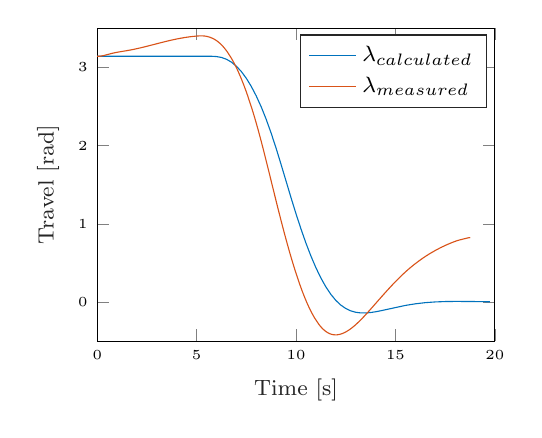
\begin{tikzpicture}

\begin{axis}[%
width=5.05cm,
height=3.975cm,
at={(0cm,0cm)},
scale only axis,
xmin=0,
xmax=20,
xlabel style={font=\color{white!15!black}},
xlabel={\footnotesize{Time [s]}},
ymin=-0.5,
ymax=3.5,
ylabel style={font=\color{white!15!black}},
ylabel={\footnotesize{Travel [rad]}},
ticklabel style = {font = \tiny},
axis background/.style={fill=white},
legend style={legend cell align=left, align=left, draw=white!15!black, font = \footnotesize}
]
\addplot [color=mycolor1]
  table[row sep=crcr]{%
0	3.14159265358979\\
5.75	3.14159265358979\\
6	3.13784214135928\\
6.25	3.12621555345474\\
6.5	3.10330930002669\\
6.75	3.0666274151879\\
7	3.01445392239088\\
7.25	2.9456562771143\\
7.5	2.8595077632903\\
7.75	2.75555158796194\\
8	2.63350511048711\\
8.25	2.49319560602897\\
8.5	2.33451857606133\\
8.75	2.15741132146842\\
9	1.9632257910249\\
9.25	1.7564180656089\\
9.75	1.3320083929786\\
10	1.12703048345801\\
10.25	0.9328551583341\\
10.5	0.75228628518121\\
10.75	0.587167239643097\\
11	0.438677564986754\\
11.25	0.307557137674021\\
11.5	0.19426300997479\\
11.75	0.0990741267562285\\
12	0.0219208065308258\\
12.25	-0.0379691069412758\\
12.5	-0.082000864322076\\
12.75	-0.112014385281746\\
13	-0.130077585103898\\
13.25	-0.138314374171593\\
13.5	-0.138777059669369\\
13.75	-0.13335998629864\\
14	-0.123747200450591\\
14.25	-0.111386469203904\\
15.5	-0.0426921073624413\\
16	-0.0219910027145644\\
16.5	-0.00725887427575245\\
17	0.00200544669756653\\
17.5	0.00687586171638443\\
18	0.00858963546312808\\
18.75	0.00769622829569272\\
19.75	0.00426248975147203\\
};
\addlegendentry{$\lambda{}_{\text{calculated}}$}

\addplot [color=mycolor2]
  table[row sep=crcr]{%
0	3.14159265358979\\
0.135999999999999	3.14235964398373\\
0.141999999999999	3.14312663437768\\
0.190000000000001	3.14389362477162\\
0.196000000000002	3.14466061516556\\
0.225999999999999	3.14542760555951\\
0.231999999999999	3.14619459595345\\
0.260000000000002	3.14696158634739\\
0.266000000000002	3.14772857674134\\
0.289999999999999	3.14849556713528\\
0.295999999999999	3.14926255752922\\
0.315999999999999	3.15002954792316\\
0.321999999999999	3.15079653831711\\
0.338000000000001	3.15156352871105\\
0.344000000000001	3.15233051910499\\
0.364000000000001	3.15309750949893\\
0.370000000000001	3.15386449989288\\
0.390000000000001	3.15463149028682\\
0.396000000000001	3.15539848068076\\
0.416	3.15616547107471\\
0.423999999999999	3.15769945186259\\
0.446000000000002	3.15846644225654\\
0.452000000000002	3.15923343265048\\
0.472000000000001	3.16000042304442\\
0.48	3.16153440383231\\
0.504000000000001	3.16230139422625\\
0.510000000000002	3.16306838462019\\
0.521999999999998	3.16383537501413\\
0.527999999999999	3.16460236540808\\
0.548000000000002	3.16536935580202\\
0.553999999999998	3.16613634619596\\
0.568000000000001	3.16690333658991\\
0.574000000000002	3.16767032698385\\
0.591999999999999	3.16843731737779\\
0.597999999999999	3.16920430777174\\
0.616	3.16997129816568\\
0.622	3.17073828855962\\
0.635999999999999	3.17150527895356\\
0.641999999999999	3.17227226934751\\
0.66	3.17303925974145\\
0.666	3.17380625013539\\
0.686	3.17457324052933\\
0.692	3.17534023092328\\
0.707999999999998	3.17610722131722\\
0.713999999999999	3.17687421171116\\
0.734000000000002	3.17764120210511\\
0.739999999999998	3.17840819249905\\
0.757999999999999	3.17917518289299\\
0.763999999999999	3.17994217328694\\
0.783999999999999	3.18070916368088\\
0.789999999999999	3.18147615407482\\
0.812000000000001	3.18224314446876\\
0.818000000000001	3.18301013486271\\
0.835999999999999	3.18377712525665\\
0.841999999999999	3.18454411565059\\
0.866	3.18531110604453\\
0.872	3.18607809643848\\
0.896000000000001	3.18684508683242\\
0.902000000000001	3.18761207722636\\
0.923999999999999	3.18837906762031\\
0.93	3.18914605801425\\
0.956	3.18991304840819\\
0.962	3.19068003880214\\
0.986000000000001	3.19144702919608\\
0.992000000000001	3.19221401959002\\
1.02	3.19298100998396\\
1.026	3.19374800037791\\
1.052	3.19451499077185\\
1.058	3.19528198116579\\
1.086	3.19604897155973\\
1.092	3.19681596195367\\
1.12	3.19758295234762\\
1.126	3.19834994274156\\
1.154	3.1991169331355\\
1.16	3.19988392352945\\
1.19	3.20065091392339\\
1.196	3.20141790431733\\
1.226	3.20218489471128\\
1.232	3.20295188510522\\
1.262	3.20371887549916\\
1.268	3.2044858658931\\
1.298	3.20525285628705\\
1.304	3.20601984668099\\
1.336	3.20678683707493\\
1.342	3.20755382746887\\
1.372	3.20832081786282\\
1.378	3.20908780825676\\
1.408	3.2098547986507\\
1.414	3.21062178904465\\
1.444	3.21138877943859\\
1.45	3.21215576983253\\
1.48	3.21292276022648\\
1.486	3.21368975062042\\
1.514	3.21445674101436\\
1.52	3.2152237314083\\
1.55	3.21599072180225\\
1.556	3.21675771219619\\
1.584	3.21752470259013\\
1.59	3.21829169298407\\
1.616	3.21905868337802\\
1.622	3.21982567377196\\
1.65	3.2205926641659\\
1.656	3.22135965455985\\
1.682	3.22212664495379\\
1.688	3.22289363534773\\
1.714	3.22366062574168\\
1.72	3.22442761613562\\
1.742	3.22519460652956\\
1.748	3.2259615969235\\
1.776	3.22672858731745\\
1.782	3.22749557771139\\
1.804	3.22826256810533\\
1.81	3.22902955849927\\
1.832	3.22979654889322\\
1.838	3.23056353928716\\
1.864	3.2313305296811\\
1.87	3.23209752007505\\
1.89	3.23286451046899\\
1.896	3.23363150086293\\
1.918	3.23439849125688\\
1.924	3.23516548165082\\
1.948	3.23593247204476\\
1.954	3.2366994624387\\
1.974	3.23746645283265\\
1.98	3.23823344322659\\
2.002	3.23900043362053\\
2.008	3.23976742401447\\
2.03	3.24053441440842\\
2.036	3.24130140480236\\
2.054	3.2420683951963\\
2.06	3.24283538559025\\
2.08	3.24360237598419\\
2.086	3.24436936637813\\
2.108	3.24513635677208\\
2.114	3.24590334716602\\
2.134	3.24667033755996\\
2.14	3.2474373279539\\
2.16	3.24820431834785\\
2.166	3.24897130874179\\
2.184	3.24973829913573\\
2.19	3.25050528952967\\
2.212	3.25127227992362\\
2.218	3.25203927031756\\
2.234	3.2528062607115\\
2.24	3.25357325110545\\
2.26	3.25434024149939\\
2.266	3.25510723189333\\
2.288	3.25587422228728\\
2.294	3.25664121268122\\
2.31	3.25740820307516\\
2.316	3.2581751934691\\
2.336	3.25894218386305\\
2.342	3.25970917425699\\
2.362	3.26047616465093\\
2.368	3.26124315504487\\
2.384	3.26201014543881\\
2.39	3.26277713583276\\
2.412	3.2635441262267\\
2.418	3.26431111662064\\
2.434	3.26507810701459\\
2.44	3.26584509740853\\
2.458	3.26661208780247\\
2.464	3.26737907819642\\
2.484	3.26814606859036\\
2.49	3.2689130589843\\
2.506	3.26968004937824\\
2.512	3.27044703977219\\
2.532	3.27121403016613\\
2.538	3.27198102056007\\
2.554	3.27274801095401\\
2.56	3.27351500134796\\
2.58	3.2742819917419\\
2.586	3.27504898213584\\
2.602	3.27581597252979\\
2.608	3.27658296292373\\
2.626	3.27734995331767\\
2.632	3.27811694371162\\
2.65	3.27888393410556\\
2.656	3.2796509244995\\
2.674	3.28041791489344\\
2.68	3.28118490528739\\
2.7	3.28195189568133\\
2.706	3.28271888607527\\
2.72	3.28348587646921\\
2.726	3.28425286686316\\
2.746	3.2850198572571\\
2.752	3.28578684765104\\
2.768	3.28655383804499\\
2.774	3.28732082843893\\
2.794	3.28808781883287\\
2.8	3.28885480922682\\
2.814	3.28962179962076\\
2.82	3.2903887900147\\
2.84	3.29115578040864\\
2.846	3.29192277080259\\
2.862	3.29268976119653\\
2.868	3.29345675159047\\
2.886	3.29422374198441\\
2.892	3.29499073237836\\
2.908	3.2957577227723\\
2.914	3.29652471316624\\
2.934	3.29729170356019\\
2.94	3.29805869395413\\
2.954	3.29882568434807\\
2.96	3.29959267474202\\
2.98	3.30035966513596\\
2.986	3.3011266555299\\
3	3.30189364592384\\
3.006	3.30266063631779\\
3.026	3.30342762671173\\
3.032	3.30419461710567\\
3.048	3.30496160749961\\
3.054	3.30572859789356\\
3.074	3.3064955882875\\
3.08	3.30726257868144\\
3.094	3.30802956907539\\
3.1	3.30879655946933\\
3.12	3.30956354986327\\
3.126	3.31033054025722\\
3.142	3.31109753065116\\
3.148	3.3118645210451\\
3.166	3.31263151143904\\
3.172	3.31339850183299\\
3.188	3.31416549222693\\
3.194	3.31493248262087\\
3.214	3.31569947301481\\
3.22	3.31646646340876\\
3.238	3.3172334538027\\
3.244	3.31800044419664\\
3.26	3.31876743459058\\
3.266	3.31953442498453\\
3.286	3.32030141537847\\
3.292	3.32106840577242\\
3.308	3.32183539616636\\
3.314	3.3226023865603\\
3.334	3.32336937695424\\
3.34	3.32413636734818\\
3.356	3.32490335774213\\
3.362	3.32567034813607\\
3.38	3.32643733853001\\
3.386	3.32720432892395\\
3.406	3.3279713193179\\
3.412	3.32873830971184\\
3.428	3.32950530010578\\
3.434	3.33027229049973\\
3.454	3.33103928089367\\
3.46	3.33180627128761\\
3.48	3.33257326168156\\
3.486	3.3333402520755\\
3.504	3.33410724246944\\
3.51	3.33487423286338\\
3.53	3.33564122325733\\
3.536	3.33640821365127\\
3.556	3.33717520404521\\
3.562	3.33794219443915\\
3.578	3.3387091848331\\
3.584	3.33947617522704\\
3.606	3.34024316562098\\
3.612	3.34101015601493\\
3.632	3.34177714640887\\
3.638	3.34254413680281\\
3.658	3.34331112719676\\
3.664	3.3440781175907\\
3.682	3.34484510798464\\
3.688	3.34561209837858\\
3.71	3.34637908877253\\
3.716	3.34714607916647\\
3.736	3.34791306956041\\
3.742	3.34868005995435\\
3.764	3.3494470503483\\
3.77	3.35021404074224\\
3.79	3.35098103113618\\
3.796	3.35174802153013\\
3.818	3.35251501192407\\
3.824	3.35328200231801\\
3.844	3.35404899271196\\
3.85	3.3548159831059\\
3.874	3.35558297349984\\
3.88	3.35634996389378\\
3.902	3.35711695428773\\
3.908	3.35788394468167\\
3.932	3.35865093507561\\
3.938	3.35941792546955\\
3.96	3.3601849158635\\
3.966	3.36095190625744\\
3.99	3.36171889665138\\
3.996	3.36248588704533\\
4.02	3.36325287743927\\
4.026	3.36401986783321\\
4.05	3.36478685822716\\
4.056	3.3655538486211\\
4.082	3.36632083901504\\
4.088	3.36708782940898\\
4.114	3.36785481980293\\
4.12	3.36862181019687\\
4.146	3.36938880059081\\
4.152	3.37015579098475\\
4.18	3.3709227813787\\
4.186	3.37168977177264\\
4.212	3.37245676216658\\
4.218	3.37322375256052\\
4.246	3.37399074295447\\
4.252	3.37475773334841\\
4.282	3.37552472374236\\
4.288	3.3762917141363\\
4.314	3.37705870453024\\
4.32	3.37782569492418\\
4.35	3.37859268531813\\
4.356	3.37935967571207\\
4.388	3.38012666610601\\
4.394	3.38089365649995\\
4.428	3.3816606468939\\
4.434	3.38242763728784\\
4.464	3.38319462768178\\
4.47	3.38396161807572\\
4.506	3.38472860846967\\
4.512	3.38549559886361\\
4.548	3.38626258925755\\
4.554	3.3870295796515\\
4.592	3.38779657004544\\
4.598	3.38856356043938\\
4.636	3.38933055083332\\
4.642	3.39009754122727\\
4.682	3.39086453162121\\
4.688	3.39163152201515\\
4.732	3.39239851240909\\
4.738	3.39316550280304\\
4.784	3.39393249319698\\
4.79	3.39469948359092\\
4.842	3.39546647398487\\
4.848	3.39623346437881\\
4.9	3.39700045477275\\
4.906	3.3977674451667\\
4.964	3.39853443556064\\
4.97	3.39930142595458\\
5.04	3.40006841634852\\
5.046	3.40083540674247\\
5.146	3.40160239713641\\
5.152	3.40236938753035\\
5.346	3.40160239713641\\
5.352	3.40083540674247\\
5.404	3.40006841634852\\
5.41	3.39930142595458\\
5.45	3.39853443556064\\
5.456	3.3977674451667\\
5.482	3.39700045477275\\
5.488	3.39623346437881\\
5.512	3.39546647398487\\
5.518	3.39469948359092\\
5.538	3.39393249319698\\
5.544	3.39316550280304\\
5.564	3.39239851240909\\
5.57	3.39163152201515\\
5.584	3.39086453162121\\
5.59	3.39009754122727\\
5.608	3.38933055083332\\
5.614	3.38856356043938\\
5.626	3.38779657004544\\
5.632	3.3870295796515\\
5.644	3.38626258925755\\
5.65	3.38549559886361\\
5.664	3.38472860846967\\
5.67	3.38396161807572\\
5.682	3.38319462768178\\
5.69	3.3816606468939\\
5.704	3.38089365649995\\
5.71	3.38012666610601\\
5.72	3.37935967571207\\
5.726	3.37859268531813\\
5.736	3.37782569492418\\
5.742	3.37705870453024\\
5.75	3.3762917141363\\
5.756	3.37552472374236\\
5.764	3.37475773334841\\
5.77	3.37399074295447\\
5.778	3.37322375256052\\
5.786	3.37168977177264\\
5.798	3.3709227813787\\
5.806	3.36938880059081\\
5.816	3.36862181019687\\
5.824	3.36708782940898\\
5.836	3.36632083901504\\
5.844	3.36478685822716\\
5.852	3.36401986783321\\
5.86	3.36248588704533\\
5.868	3.36171889665138\\
5.876	3.3601849158635\\
5.886	3.35941792546955\\
5.894	3.35788394468167\\
5.902	3.35711695428773\\
5.91	3.35558297349984\\
5.916	3.3548159831059\\
5.924	3.35328200231801\\
5.932	3.35251501192407\\
5.94	3.35098103113618\\
5.946	3.35021404074224\\
5.954	3.34868005995435\\
5.96	3.34791306956041\\
5.968	3.34637908877253\\
5.974	3.34561209837858\\
5.982	3.3440781175907\\
5.988	3.34331112719676\\
5.996	3.34177714640887\\
6	3.34101015601493\\
6.008	3.33947617522704\\
6.014	3.3387091848331\\
6.022	3.33717520404521\\
6.026	3.33640821365127\\
6.034	3.33487423286338\\
6.04	3.33410724246944\\
6.05	3.33180627128761\\
6.056	3.33103928089367\\
6.066	3.32873830971184\\
6.07	3.3279713193179\\
6.078	3.32643733853001\\
6.082	3.32567034813607\\
6.092	3.32336937695424\\
6.098	3.3226023865603\\
6.108	3.32030141537847\\
6.112	3.31953442498453\\
6.122	3.3172334538027\\
6.126	3.31646646340876\\
6.136	3.31416549222693\\
6.14	3.31339850183299\\
6.15	3.31109753065116\\
6.154	3.31033054025722\\
6.164	3.30802956907539\\
6.168	3.30726257868144\\
6.18	3.30419461710567\\
6.184	3.30342762671173\\
6.196	3.30035966513596\\
6.2	3.29959267474202\\
6.212	3.29652471316624\\
6.216	3.2957577227723\\
6.23	3.29192277080259\\
6.236	3.29115578040864\\
6.252	3.28655383804499\\
6.256	3.28578684765104\\
6.272	3.28118490528739\\
6.278	3.28041791489344\\
6.298	3.2742819917419\\
6.302	3.27351500134796\\
6.318	3.2689130589843\\
6.322	3.26814606859036\\
6.342	3.26201014543881\\
6.346	3.26124315504487\\
6.366	3.25510723189333\\
6.37	3.25434024149939\\
6.394	3.24667033755996\\
6.398	3.24590334716602\\
6.428	3.23593247204476\\
6.432	3.23516548165082\\
6.466	3.22366062574168\\
6.47	3.22289363534773\\
6.522	3.2044858658931\\
6.526	3.20371887549916\\
6.736	3.12165090334728\\
6.742	3.11858294177151\\
6.778	3.10324313389265\\
6.784	3.10017517231688\\
6.812	3.08790332601379\\
6.818	3.08483536443802\\
6.84	3.07486448931677\\
6.846	3.071796527741\\
6.866	3.06259264301368\\
6.872	3.05952468143791\\
6.89	3.05108778710454\\
6.898	3.04648584474088\\
6.918	3.03728196001357\\
6.926	3.03268001764991\\
6.944	3.02424312331654\\
6.952	3.01964118095288\\
6.968	3.01197127701346\\
6.976	3.0073693346498\\
6.99	3.00046642110431\\
6.998	2.99586447874066\\
7.012	2.98896156519517\\
7.02	2.98435962283152\\
7.032	2.97822369967997\\
7.04	2.97362175731632\\
7.052	2.96748583416477\\
7.062	2.96134991101323\\
7.074	2.95521398786169\\
7.082	2.95061204549803\\
7.09	2.94601010313437\\
7.098	2.94140816077072\\
7.108	2.93603922801312\\
7.118	2.92990330486158\\
7.13	2.92376738171003\\
7.14	2.91763145855849\\
7.148	2.91302951619483\\
7.158	2.90689359304329\\
7.168	2.90152466028569\\
7.18	2.89385475634626\\
7.19	2.88848582358866\\
7.202	2.88081591964923\\
7.21	2.87621397728558\\
7.22	2.87007805413403\\
7.228	2.86547611177038\\
7.24	2.85780620783095\\
7.248	2.85320426546729\\
7.26	2.84553436152786\\
7.268	2.84093241916421\\
7.284	2.83019455364901\\
7.292	2.82559261128535\\
7.306	2.81638872655804\\
7.312	2.81255377458832\\
7.326	2.80334988986101\\
7.334	2.79874794749735\\
7.352	2.78647610119427\\
7.358	2.78264114922455\\
7.374	2.77190328370935\\
7.382	2.7673013413457\\
7.406	2.75042755267895\\
7.412	2.74659260070924\\
7.432	2.73278677361827\\
7.438	2.72895182164856\\
7.462	2.71207803298181\\
7.468	2.7082430810121\\
7.498	2.6867673499817\\
7.504	2.68293239801199\\
7.544	2.65378676304216\\
7.55	2.64995181107244\\
7.796	2.45973819337463\\
7.804	2.45283527982914\\
7.836	2.42675760643509\\
7.844	2.4198546928896\\
7.868	2.39991294264708\\
7.876	2.3930100291016\\
7.896	2.37613624043486\\
7.904	2.36923332688937\\
7.922	2.35389351901052\\
7.932	2.3446896342832\\
7.952	2.32781584561646\\
7.962	2.31861196088915\\
7.98	2.30327215301029\\
7.99	2.29406826828298\\
8.006	2.280262441192\\
8.016	2.27105855646469\\
8.028	2.26032069094949\\
8.038	2.25111680622218\\
8.052	2.23884495991909\\
8.062	2.22964107519178\\
8.072	2.22043719046447\\
8.082	2.21123330573715\\
8.094	2.20049544022195\\
8.106	2.18899058431281\\
8.116	2.1797866995855\\
8.128	2.16828184367635\\
8.14	2.15754397816115\\
8.152	2.14603912225201\\
8.164	2.13530125673681\\
8.178	2.12149542964584\\
8.188	2.11229154491853\\
8.202	2.09848571782756\\
8.212	2.08928183310024\\
8.226	2.07547600600927\\
8.236	2.06627212128196\\
8.25	2.05246629419099\\
8.26	2.04326240946368\\
8.276	2.02715561119087\\
8.286	2.01795172646356\\
8.302	2.00184492819076\\
8.31	1.99417502425133\\
8.326	1.97806822597854\\
8.336	1.96886434125122\\
8.354	1.95045657179659\\
8.362	1.94278666785716\\
8.378	1.92667986958437\\
8.386	1.91900996564494\\
8.404	1.90060219619031\\
8.412	1.89293229225088\\
8.432	1.87222355161443\\
8.44	1.864553647675\\
8.46	1.84384490703854\\
8.468	1.83617500309911\\
8.488	1.81546626246266\\
8.496	1.80779635852323\\
8.518	1.78478664670494\\
8.526	1.77711674276551\\
8.546	1.75640800212906\\
8.554	1.74873809818963\\
8.578	1.72342741518952\\
8.586	1.71575751125009\\
8.608	1.69274779943181\\
8.616	1.68507789549238\\
8.64	1.65976721249226\\
8.648	1.65209730855284\\
8.672	1.62678662555272\\
8.68	1.6191167216133\\
8.704	1.59380603861318\\
8.712	1.58613613467375\\
8.736	1.56082545167364\\
8.744	1.55315554773421\\
8.77	1.52554389355227\\
8.778	1.51787398961284\\
8.802	1.49256330661273\\
8.81	1.4848934026733\\
8.834	1.45958271967319\\
8.842	1.45191281573376\\
8.866	1.42660213273365\\
8.874	1.41893222879422\\
8.898	1.3936215457941\\
8.906	1.38595164185468\\
8.93	1.36064095885456\\
8.938	1.35297105491513\\
8.96	1.32996134309685\\
8.968	1.32229143915742\\
8.99	1.29928172733914\\
8.998	1.29161182339971\\
9.02	1.26860211158143\\
9.028	1.260932207642\\
9.048	1.24022346700554\\
9.056	1.23255356306611\\
9.076	1.21184482242966\\
9.084	1.20417491849023\\
9.104	1.18346617785377\\
9.112	1.17579627391434\\
9.13	1.15738850445972\\
9.138	1.14971860052029\\
9.156	1.13131083106566\\
9.164	1.12364092712623\\
9.182	1.10523315767161\\
9.19	1.09756325373218\\
9.206	1.08145645545938\\
9.214	1.07378655151995\\
9.23	1.05767975324715\\
9.238	1.05000984930772\\
9.254	1.03390305103492\\
9.262	1.02623314709549\\
9.278	1.01012634882269\\
9.288	1.00092246409538\\
9.304	0.98481566582258\\
9.314	0.975611781095267\\
9.33	0.95950498282247\\
9.34	0.950301098095157\\
9.354	0.936495271004183\\
9.364	0.92729138627687\\
9.38	0.911184588004073\\
9.39	0.901980703276756\\
9.402	0.890475847367615\\
9.412	0.881271962640302\\
9.426	0.867466135549328\\
9.436	0.858262250822015\\
9.448	0.846757394912874\\
9.458	0.837553510185561\\
9.47	0.826048654276416\\
9.48	0.816844769549103\\
9.492	0.805339913639962\\
9.504	0.794602048124762\\
9.516	0.783097192215621\\
9.528	0.772359326700421\\
9.54	0.76085447079128\\
9.552	0.75011660527608\\
9.564	0.738611749366935\\
9.578	0.726339903063852\\
9.588	0.717136018336536\\
9.6	0.70639815282134\\
9.612	0.694893296912195\\
9.628	0.681087469821225\\
9.638	0.671883585093912\\
9.652	0.659611738790826\\
9.662	0.650407854063513\\
9.678	0.63660202697254\\
9.688	0.627398142245227\\
9.704	0.613592315154257\\
9.714	0.604388430426944\\
9.734	0.587514641760201\\
9.744	0.578310757032888\\
9.766	0.559902987578258\\
9.776	0.550699102850945\\
9.8	0.530757352608433\\
9.808	0.523854439062948\\
9.83	0.505446669608318\\
9.838	0.498543756062833\\
9.866	0.475534044244547\\
9.874	0.468631130699062\\
9.908	0.441019476517123\\
9.916	0.434116562971635\\
9.972	0.389631120122953\\
9.98	0.382728206577468\\
10.172	0.237000031728332\\
10.178	0.233165079758617\\
10.216	0.205553425576674\\
10.222	0.201718473606963\\
10.252	0.180242742576564\\
10.258	0.176407790606849\\
10.282	0.159534001940106\\
10.288	0.155699049970394\\
10.308	0.141893222879421\\
10.314	0.138058270909706\\
10.332	0.125786424606623\\
10.338	0.121951472636908\\
10.354	0.111213607121709\\
10.362	0.106611664758052\\
10.38	0.0943398184549658\\
10.388	0.0897378760913092\\
10.404	0.0790000105761095\\
10.41	0.0751650586063981\\
10.422	0.0674951546669682\\
10.43	0.0628932123033117\\
10.444	0.0536893275759986\\
10.452	0.0490873852123421\\
10.464	0.0414174812729122\\
10.472	0.0368155389092557\\
10.484	0.0291456349698258\\
10.492	0.0245436926061693\\
10.504	0.0168737886667429\\
10.514	0.0115048559091413\\
10.526	0.00383495196971495\\
10.536	-0.00153398078788669\\
10.546	-0.0076699039394299\\
10.554	-0.0122718463030864\\
10.564	-0.0184077694546296\\
10.574	-0.0237767022122277\\
10.582	-0.0283786445758842\\
10.592	-0.0337475773334859\\
10.602	-0.0398835004850255\\
10.614	-0.0460194236365687\\
10.624	-0.052155346788112\\
10.636	-0.0582912699396552\\
10.644	-0.0628932123033117\\
10.656	-0.0690291354548549\\
10.664	-0.0736310778185114\\
10.676	-0.0797670009700546\\
10.684	-0.0843689433337111\\
10.698	-0.0912718568791959\\
10.706	-0.0958737992428524\\
10.72	-0.102776712788337\\
10.728	-0.107378655151994\\
10.746	-0.115815549485365\\
10.754	-0.120417491849022\\
10.774	-0.129621376576338\\
10.782	-0.134223318939995\\
10.804	-0.144194194061249\\
10.81	-0.147262155637023\\
10.83	-0.156466040364336\\
10.836	-0.159534001940106\\
10.86	-0.170271867455305\\
10.866	-0.173339829031079\\
10.894	-0.185611675334162\\
10.9	-0.188679636909935\\
10.946	-0.207854396758506\\
10.952	-0.210922358334276\\
11.152	-0.286087416940671\\
11.156	-0.286854407334616\\
11.188	-0.297592272849815\\
11.192	-0.298359263243757\\
11.22	-0.30756314797107\\
11.224	-0.308330138365015\\
11.246	-0.3152330519105\\
11.25	-0.316000042304442\\
11.272	-0.322902955849926\\
11.276	-0.323669946243871\\
11.292	-0.328271888607528\\
11.296	-0.32903887900147\\
11.312	-0.333640821365126\\
11.316	-0.334407811759071\\
11.33	-0.338242763728783\\
11.334	-0.339009754122728\\
11.348	-0.342844706092443\\
11.352	-0.343611696486384\\
11.366	-0.347446648456099\\
11.372	-0.348213638850041\\
11.386	-0.352048590819756\\
11.392	-0.352815581213697\\
11.406	-0.356650533183412\\
11.412	-0.357417523577354\\
11.424	-0.360485485153127\\
11.43	-0.361252475547069\\
11.442	-0.364320437122839\\
11.448	-0.365087427516784\\
11.46	-0.368155389092554\\
11.466	-0.368922379486499\\
11.476	-0.371223350668327\\
11.482	-0.371990341062268\\
11.492	-0.374291312244097\\
11.498	-0.375058302638038\\
11.506	-0.376592283425925\\
11.512	-0.377359273819867\\
11.522	-0.379660245001695\\
11.528	-0.38042723539564\\
11.536	-0.381961216183527\\
11.542	-0.382728206577468\\
11.55	-0.384262187365355\\
11.556	-0.385029177759296\\
11.564	-0.386563158547183\\
11.57	-0.387330148941125\\
11.578	-0.388864129729011\\
11.586	-0.389631120122953\\
11.594	-0.39116510091084\\
11.602	-0.391932091304781\\
11.61	-0.393466072092668\\
11.618	-0.394233062486609\\
11.624	-0.395000052880555\\
11.63	-0.395767043274496\\
11.638	-0.397301024062383\\
11.648	-0.398068014456324\\
11.656	-0.399601995244211\\
11.668	-0.400368985638153\\
11.676	-0.401902966426039\\
11.688	-0.402669956819981\\
11.694	-0.403436947213923\\
11.702	-0.404203937607868\\
11.708	-0.404970928001809\\
11.718	-0.405737918395751\\
11.724	-0.406504908789696\\
11.734	-0.407271899183637\\
11.74	-0.408038889577583\\
11.754	-0.408805879971524\\
11.76	-0.409572870365466\\
11.772	-0.410339860759411\\
11.778	-0.411106851153352\\
11.792	-0.411873841547294\\
11.798	-0.412640831941239\\
11.816	-0.413407822335181\\
11.822	-0.414174812729122\\
11.844	-0.414941803123067\\
11.85	-0.415708793517009\\
11.882	-0.416475783910951\\
11.888	-0.417242774304896\\
11.94	-0.418009764698837\\
11.946	-0.418776755092779\\
12.076	-0.418009764698837\\
12.082	-0.417242774304896\\
12.118	-0.416475783910951\\
12.124	-0.415708793517009\\
12.152	-0.414941803123067\\
12.158	-0.414174812729122\\
12.18	-0.413407822335181\\
12.186	-0.412640831941239\\
12.206	-0.411873841547294\\
12.212	-0.411106851153352\\
12.228	-0.410339860759411\\
12.234	-0.409572870365466\\
12.248	-0.408805879971524\\
12.254	-0.408038889577583\\
12.266	-0.407271899183637\\
12.272	-0.406504908789696\\
12.286	-0.405737918395751\\
12.292	-0.404970928001809\\
12.304	-0.404203937607868\\
12.312	-0.402669956819981\\
12.326	-0.401902966426039\\
12.332	-0.401135976032094\\
12.342	-0.400368985638153\\
12.348	-0.399601995244211\\
12.356	-0.398835004850266\\
12.362	-0.398068014456324\\
12.372	-0.397301024062383\\
12.378	-0.396534033668438\\
12.386	-0.395767043274496\\
12.392	-0.395000052880555\\
12.398	-0.394233062486609\\
12.404	-0.393466072092668\\
12.412	-0.392699081698723\\
12.418	-0.391932091304781\\
12.426	-0.39116510091084\\
12.434	-0.389631120122953\\
12.444	-0.388864129729011\\
12.452	-0.387330148941125\\
12.462	-0.386563158547183\\
12.47	-0.385029177759296\\
12.48	-0.384262187365355\\
12.488	-0.382728206577468\\
12.496	-0.381961216183527\\
12.504	-0.38042723539564\\
12.514	-0.379660245001695\\
12.522	-0.378126264213812\\
12.53	-0.377359273819867\\
12.538	-0.375825293031983\\
12.544	-0.375058302638038\\
12.552	-0.373524321850155\\
12.56	-0.37275733145621\\
12.568	-0.371223350668327\\
12.576	-0.370456360274382\\
12.584	-0.368922379486499\\
12.59	-0.368155389092554\\
12.598	-0.366621408304667\\
12.604	-0.365854417910725\\
12.612	-0.364320437122839\\
12.618	-0.363553446728897\\
12.626	-0.36201946594101\\
12.632	-0.361252475547069\\
12.64	-0.359718494759182\\
12.646	-0.35895150436524\\
12.654	-0.357417523577354\\
12.66	-0.356650533183412\\
12.668	-0.355116552395526\\
12.674	-0.354349562001584\\
12.684	-0.352048590819756\\
12.692	-0.351281600425811\\
12.702	-0.348980629243982\\
12.708	-0.348213638850041\\
12.716	-0.346679658062154\\
12.722	-0.345912667668212\\
12.732	-0.343611696486384\\
12.738	-0.342844706092443\\
12.748	-0.340543734910614\\
12.754	-0.339776744516669\\
12.764	-0.337475773334841\\
12.77	-0.336708782940899\\
12.78	-0.334407811759071\\
12.786	-0.333640821365126\\
12.796	-0.331339850183298\\
12.802	-0.330572859789356\\
12.812	-0.328271888607528\\
12.818	-0.327504898213586\\
12.828	-0.325203927031755\\
12.834	-0.324436936637813\\
12.846	-0.321368975062043\\
12.852	-0.320601984668098\\
12.862	-0.31830101348627\\
12.866	-0.317534023092328\\
12.876	-0.3152330519105\\
12.882	-0.314466061516558\\
12.894	-0.311398099940785\\
12.9	-0.310631109546843\\
12.912	-0.30756314797107\\
12.918	-0.306796157577129\\
12.93	-0.303728196001359\\
12.936	-0.302961205607414\\
12.948	-0.299893244031644\\
12.952	-0.299126253637699\\
12.962	-0.29682528245587\\
12.966	-0.296058292061929\\
12.976	-0.293757320880101\\
12.98	-0.292990330486159\\
12.99	-0.290689359304331\\
12.994	-0.289922368910386\\
13.006	-0.286854407334616\\
13.012	-0.286087416940671\\
13.026	-0.282252464970959\\
13.032	-0.281485474577014\\
13.046	-0.277650522607303\\
13.052	-0.276883532213358\\
13.066	-0.273048580243646\\
13.07	-0.272281589849701\\
13.082	-0.269213628273931\\
13.086	-0.268446637879986\\
13.098	-0.265378676304216\\
13.102	-0.264611685910275\\
13.114	-0.261543724334501\\
13.118	-0.26077673394056\\
13.13	-0.257708772364786\\
13.134	-0.256941781970845\\
13.146	-0.253873820395075\\
13.15	-0.25310683000113\\
13.164	-0.249271878031418\\
13.168	-0.248504887637473\\
13.18	-0.245436926061704\\
13.184	-0.244669935667758\\
13.198	-0.240834983698047\\
13.202	-0.240067993304102\\
13.216	-0.23623304133439\\
13.222	-0.235466050940445\\
13.238	-0.230864108576789\\
13.242	-0.230097118182847\\
13.256	-0.226262166213132\\
13.26	-0.225495175819191\\
13.276	-0.220893233455534\\
13.282	-0.220126243061589\\
13.3	-0.214757310303991\\
13.304	-0.213990319910046\\
13.318	-0.210155367940335\\
13.322	-0.209388377546389\\
13.338	-0.204786435182733\\
13.342	-0.204019444788791\\
13.356	-0.200184492819076\\
13.36	-0.199417502425135\\
13.376	-0.194815560061478\\
13.38	-0.194048569667533\\
13.396	-0.189446627303877\\
13.4	-0.188679636909935\\
13.416	-0.184077694546279\\
13.42	-0.183310704152333\\
13.436	-0.178708761788677\\
13.44	-0.177941771394735\\
13.456	-0.173339829031079\\
13.46	-0.172572838637134\\
13.48	-0.166436915485594\\
13.484	-0.165669925091649\\
13.5	-0.161067982727992\\
13.504	-0.160300992334051\\
13.522	-0.154932059576449\\
13.526	-0.154165069182508\\
13.542	-0.149563126818851\\
13.546	-0.148796136424906\\
13.564	-0.143427203667308\\
13.568	-0.142660213273366\\
13.586	-0.137291280515765\\
13.59	-0.136524290121823\\
13.61	-0.13038836697028\\
13.614	-0.129621376576338\\
13.632	-0.124252443818737\\
13.636	-0.123485453424795\\
13.656	-0.117349530273252\\
13.66	-0.11658253987931\\
13.678	-0.111213607121709\\
13.682	-0.110446616727767\\
13.702	-0.104310693576224\\
13.706	-0.103543703182282\\
13.726	-0.0974077800307391\\
13.73	-0.096640789636794\\
13.748	-0.0912718568791959\\
13.752	-0.0905048664852544\\
13.772	-0.0843689433337111\\
13.776	-0.083601952939766\\
13.796	-0.0774660297882264\\
13.8	-0.0766990393942812\\
13.82	-0.070563116242738\\
13.824	-0.0697961258487965\\
13.844	-0.0636602026972533\\
13.848	-0.0628932123033117\\
13.87	-0.0559902987578269\\
13.874	-0.0552233083638818\\
13.892	-0.0498543756062837\\
13.896	-0.0490873852123421\\
13.918	-0.0421844716668538\\
13.922	-0.0414174812729122\\
13.942	-0.035281558121369\\
13.946	-0.0345145677274274\\
13.966	-0.0283786445758842\\
13.97	-0.0276116541819427\\
13.992	-0.0207087406364579\\
13.996	-0.0199417502425128\\
14.016	-0.0138058270909696\\
14.02	-0.013038836697028\\
14.04	-0.00690291354548478\\
14.044	-0.00613592315154321\\
14.066	0.000766990393941569\\
14.07	0.00153398078788669\\
14.09	0.0076699039394299\\
14.094	0.00843689433337147\\
14.114	0.0145728174849147\\
14.118	0.0153398078788562\\
14.14	0.022242721424341\\
14.144	0.0230097118182861\\
14.164	0.0291456349698258\\
14.168	0.0299126253637709\\
14.188	0.0360485485153141\\
14.192	0.0368155389092557\\
14.212	0.0429514620607989\\
14.216	0.0437184524547405\\
14.236	0.0498543756062837\\
14.24	0.0506213660002253\\
14.26	0.0567572891517685\\
14.264	0.05752427954571\\
14.284	0.0636602026972533\\
14.288	0.0644271930911984\\
14.308	0.070563116242738\\
14.312	0.0713301066366832\\
14.33	0.0766990393942812\\
14.334	0.0774660297882264\\
14.354	0.083601952939766\\
14.358	0.0843689433337111\\
14.378	0.0905048664852544\\
14.382	0.0912718568791959\\
14.4	0.096640789636794\\
14.404	0.0974077800307391\\
14.424	0.103543703182282\\
14.428	0.104310693576224\\
14.446	0.109679626333822\\
14.45	0.110446616727767\\
14.47	0.11658253987931\\
14.474	0.117349530273252\\
14.492	0.12271846303085\\
14.496	0.123485453424795\\
14.516	0.129621376576338\\
14.52	0.13038836697028\\
14.538	0.135757299727878\\
14.542	0.136524290121823\\
14.56	0.141893222879421\\
14.564	0.142660213273366\\
14.582	0.148029146030964\\
14.586	0.148796136424906\\
14.604	0.154165069182508\\
14.608	0.154932059576449\\
14.626	0.160300992334051\\
14.63	0.161067982727992\\
14.648	0.16643691548559\\
14.652	0.167203905879536\\
14.67	0.172572838637134\\
14.674	0.173339829031079\\
14.69	0.177941771394735\\
14.694	0.178708761788677\\
14.712	0.184077694546279\\
14.716	0.18484468494022\\
14.732	0.189446627303877\\
14.736	0.190213617697818\\
14.756	0.196349540849361\\
14.76	0.197116531243307\\
14.776	0.201718473606963\\
14.78	0.202485464000905\\
14.798	0.207854396758506\\
14.802	0.208621387152448\\
14.816	0.212456339122163\\
14.82	0.213223329516104\\
14.838	0.218592262273702\\
14.842	0.219359252667648\\
14.858	0.223961195031304\\
14.862	0.224728185425246\\
14.878	0.229330127788902\\
14.882	0.230097118182847\\
14.898	0.234699060546504\\
14.902	0.235466050940445\\
14.918	0.240067993304102\\
14.922	0.240834983698047\\
14.936	0.244669935667758\\
14.94	0.245436926061704\\
14.956	0.25003886842536\\
14.96	0.250805858819302\\
14.976	0.255407801182958\\
14.982	0.256174791576903\\
15	0.261543724334501\\
15.004	0.262310714728446\\
15.018	0.266145666698158\\
15.022	0.266912657092103\\
15.038	0.27151459945576\\
15.042	0.272281589849701\\
15.056	0.276116541819416\\
15.06	0.276883532213358\\
15.074	0.280718484183073\\
15.078	0.281485474577014\\
15.094	0.286087416940671\\
15.1	0.286854407334616\\
15.116	0.291456349698272\\
15.12	0.292223340092214\\
15.134	0.296058292061929\\
15.138	0.29682528245587\\
15.152	0.300660234425585\\
15.156	0.301427224819527\\
15.17	0.305262176789242\\
15.176	0.306029167183187\\
15.192	0.310631109546843\\
15.196	0.311398099940785\\
15.21	0.3152330519105\\
15.214	0.316000042304442\\
15.228	0.319834994274157\\
15.234	0.320601984668098\\
15.25	0.325203927031755\\
15.254	0.3259709174257\\
15.266	0.32903887900147\\
15.27	0.329805869395415\\
15.284	0.333640821365126\\
15.29	0.334407811759071\\
15.304	0.338242763728783\\
15.308	0.339009754122728\\
15.322	0.342844706092443\\
15.326	0.343611696486384\\
15.338	0.346679658062154\\
15.342	0.347446648456099\\
15.354	0.350514610031869\\
15.358	0.351281600425811\\
15.37	0.354349562001584\\
15.374	0.355116552395526\\
15.386	0.358184513971299\\
15.39	0.35895150436524\\
15.402	0.36201946594101\\
15.408	0.362786456334955\\
15.422	0.366621408304667\\
15.426	0.367388398698612\\
15.438	0.370456360274382\\
15.442	0.371223350668327\\
15.454	0.374291312244097\\
15.458	0.375058302638038\\
15.47	0.378126264213812\\
15.476	0.378893254607753\\
15.49	0.382728206577468\\
15.496	0.38349519697141\\
15.51	0.387330148941125\\
15.516	0.388097139335066\\
15.53	0.391932091304781\\
15.534	0.392699081698723\\
15.544	0.395000052880551\\
15.548	0.395767043274496\\
15.558	0.398068014456324\\
15.562	0.398835004850266\\
15.574	0.401902966426039\\
15.58	0.402669956819981\\
15.594	0.406504908789696\\
15.6	0.407271899183637\\
15.612	0.410339860759411\\
15.616	0.411106851153352\\
15.626	0.413407822335181\\
15.63	0.414174812729122\\
15.64	0.416475783910951\\
15.644	0.417242774304896\\
15.654	0.419543745486724\\
15.658	0.420310735880665\\
15.668	0.422611707062494\\
15.672	0.423378697456439\\
15.682	0.425679668638267\\
15.686	0.426446659032209\\
15.696	0.428747630214037\\
15.7	0.429514620607979\\
15.71	0.431815591789807\\
15.714	0.432582582183752\\
15.724	0.43488355336558\\
15.73	0.435650543759522\\
15.742	0.438718505335295\\
15.746	0.439485495729237\\
15.756	0.441786466911065\\
15.762	0.442553457305007\\
15.774	0.44562141888078\\
15.78	0.446388409274721\\
15.792	0.449456370850491\\
15.798	0.450223361244436\\
15.81	0.453291322820206\\
15.816	0.454058313214151\\
15.826	0.45635928439598\\
15.83	0.457126274789921\\
15.84	0.459427245971749\\
15.846	0.460194236365691\\
15.856	0.462495207547519\\
15.86	0.463262197941464\\
15.87	0.465563169123293\\
15.876	0.466330159517234\\
15.886	0.468631130699062\\
15.89	0.469398121093008\\
15.9	0.471699092274836\\
15.906	0.472466082668777\\
15.916	0.474767053850606\\
15.92	0.475534044244547\\
15.93	0.477835015426379\\
15.936	0.478602005820321\\
15.946	0.480902977002149\\
15.952	0.48166996739609\\
15.962	0.483970938577919\\
15.966	0.484737928971864\\
15.976	0.487038900153692\\
15.982	0.487805890547634\\
15.992	0.490106861729462\\
15.998	0.490873852123407\\
16.008	0.493174823305235\\
16.014	0.493941813699177\\
16.024	0.496242784881005\\
16.03	0.497009775274947\\
16.04	0.499310746456775\\
16.046	0.50007773685072\\
16.056	0.502378708032548\\
16.062	0.50314569842649\\
16.072	0.505446669608318\\
16.078	0.506213660002263\\
16.088	0.508514631184092\\
16.092	0.509281621578033\\
16.102	0.511582592759861\\
16.11	0.512349583153803\\
16.12	0.514650554335631\\
16.126	0.515417544729576\\
16.136	0.517718515911405\\
16.142	0.518485506305346\\
16.152	0.520786477487174\\
16.158	0.52155346788112\\
16.168	0.523854439062948\\
16.174	0.524621429456889\\
16.184	0.526922400638718\\
16.19	0.527689391032659\\
16.198	0.529223371820546\\
16.204	0.529990362214487\\
16.214	0.532291333396319\\
16.22	0.533058323790261\\
16.23	0.535359294972089\\
16.238	0.536126285366031\\
16.248	0.538427256547859\\
16.254	0.539194246941804\\
16.264	0.541495218123632\\
16.272	0.542262208517574\\
16.282	0.544563179699402\\
16.288	0.545330170093347\\
16.298	0.547631141275176\\
16.306	0.548398131669117\\
16.316	0.550699102850945\\
16.322	0.551466093244887\\
16.33	0.553000074032774\\
16.334	0.553767064426715\\
16.342	0.555301045214602\\
16.348	0.556068035608543\\
16.356	0.55760201639643\\
16.362	0.558369006790375\\
16.372	0.560669977972204\\
16.378	0.561436968366145\\
16.386	0.562970949154032\\
16.392	0.563737939547973\\
16.4	0.56527192033586\\
16.406	0.566038910729802\\
16.416	0.56833988191163\\
16.422	0.569106872305571\\
16.43	0.570640853093458\\
16.436	0.571407843487403\\
16.444	0.572941824275286\\
16.45	0.573708814669232\\
16.458	0.575242795457115\\
16.464	0.57600978585106\\
16.474	0.578310757032888\\
16.482	0.57907774742683\\
16.492	0.581378718608658\\
16.5	0.582145709002599\\
16.51	0.584446680184428\\
16.518	0.585213670578373\\
16.526	0.58674765136626\\
16.532	0.587514641760201\\
16.542	0.589815612942029\\
16.55	0.590582603335971\\
16.558	0.592116584123858\\
16.564	0.592883574517799\\
16.572	0.594417555305686\\
16.578	0.595184545699627\\
16.586	0.596718526487514\\
16.594	0.597485516881456\\
16.604	0.599786488063287\\
16.612	0.600553478457229\\
16.62	0.602087459245116\\
16.626	0.602854449639057\\
16.634	0.604388430426944\\
16.64	0.605155420820886\\
16.648	0.606689401608772\\
16.654	0.607456392002714\\
16.662	0.608990372790601\\
16.67	0.609757363184542\\
16.678	0.611291343972429\\
16.684	0.61205833436637\\
16.692	0.613592315154257\\
16.698	0.614359305548199\\
16.706	0.615893286336085\\
16.714	0.616660276730027\\
16.722	0.618194257517914\\
16.728	0.618961247911855\\
16.736	0.620495228699742\\
16.744	0.621262219093683\\
16.752	0.62279619988157\\
16.758	0.623563190275512\\
16.766	0.625097171063398\\
16.774	0.625864161457343\\
16.782	0.627398142245227\\
16.788	0.628165132639172\\
16.796	0.629699113427055\\
16.804	0.630466103821\\
16.812	0.632000084608883\\
16.82	0.632767075002828\\
16.828	0.634301055790711\\
16.834	0.635068046184657\\
16.842	0.63660202697254\\
16.85	0.637369017366485\\
16.858	0.638902998154371\\
16.866	0.639669988548313\\
16.874	0.6412039693362\\
16.882	0.641970959730141\\
16.89	0.643504940518028\\
16.898	0.64427193091197\\
16.906	0.645805911699856\\
16.914	0.646572902093798\\
16.922	0.648106882881684\\
16.93	0.648873873275626\\
16.938	0.650407854063513\\
16.946	0.651174844457454\\
16.954	0.652708825245341\\
16.962	0.653475815639283\\
16.97	0.655009796427169\\
16.978	0.655776786821111\\
16.986	0.657310767608998\\
16.994	0.658077758002939\\
17.002	0.659611738790826\\
17.01	0.660378729184767\\
17.018	0.661912709972654\\
17.026	0.662679700366596\\
17.034	0.664213681154482\\
17.044	0.664980671548424\\
17.052	0.666514652336311\\
17.06	0.667281642730256\\
17.068	0.668815623518139\\
17.076	0.669582613912084\\
17.084	0.671116594699967\\
17.094	0.671883585093912\\
17.102	0.673417565881795\\
17.11	0.67418455627574\\
17.118	0.675718537063624\\
17.128	0.676485527457569\\
17.136	0.678019508245452\\
17.146	0.678786498639397\\
17.154	0.680320479427284\\
17.162	0.681087469821225\\
17.17	0.682621450609112\\
17.18	0.683388441003054\\
17.188	0.68492242179094\\
17.198	0.685689412184882\\
17.206	0.687223392972768\\
17.214	0.68799038336671\\
17.22	0.688757373760652\\
17.228	0.689524364154597\\
17.236	0.69105834494248\\
17.244	0.691825335336425\\
17.25	0.692592325730367\\
17.256	0.693359316124312\\
17.264	0.694893296912195\\
17.274	0.69566028730614\\
17.282	0.697194268094023\\
17.292	0.697961258487968\\
17.298	0.69872824888191\\
17.304	0.699495239275851\\
17.31	0.700262229669796\\
17.318	0.701029220063738\\
17.326	0.702563200851625\\
17.336	0.703330191245566\\
17.344	0.704864172033453\\
17.354	0.705631162427395\\
17.362	0.707165143215281\\
17.374	0.707932133609223\\
17.382	0.709466114397109\\
17.392	0.710233104791051\\
17.398	0.711000095184996\\
17.404	0.711767085578938\\
17.41	0.712534075972879\\
17.418	0.713301066366824\\
17.426	0.714835047154708\\
17.436	0.715602037548653\\
17.442	0.716369027942594\\
17.45	0.717136018336536\\
17.458	0.718669999124423\\
17.47	0.719436989518368\\
17.478	0.720970970306251\\
17.49	0.721737960700196\\
17.498	0.723271941488079\\
17.508	0.724038931882024\\
17.514	0.724805922275966\\
17.522	0.725572912669907\\
17.53	0.727106893457794\\
17.542	0.727873883851736\\
17.55	0.729407864639622\\
17.562	0.730174855033564\\
17.57	0.731708835821451\\
17.582	0.732475826215392\\
17.59	0.734009807003279\\
17.602	0.734776797397224\\
17.608	0.735543787791165\\
17.616	0.736310778185107\\
17.624	0.737844758972994\\
17.638	0.738611749366935\\
17.646	0.740145730154822\\
17.658	0.740912720548764\\
17.664	0.741679710942709\\
17.672	0.74244670133665\\
17.678	0.743213691730592\\
17.686	0.743980682124537\\
17.692	0.744747672518479\\
17.7	0.74551466291242\\
17.706	0.746281653306365\\
17.714	0.747048643700307\\
17.72	0.747815634094252\\
17.728	0.748582624488193\\
17.734	0.749349614882135\\
17.744	0.75011660527608\\
17.75	0.750883595670022\\
17.758	0.751650586063963\\
17.764	0.752417576457908\\
17.772	0.75318456685185\\
17.778	0.753951557245792\\
17.786	0.754718547639737\\
17.792	0.755485538033678\\
17.802	0.75625252842762\\
17.808	0.757019518821565\\
17.816	0.757786509215506\\
17.822	0.758553499609448\\
17.832	0.759320490003393\\
17.838	0.760087480397335\\
17.846	0.76085447079128\\
17.852	0.761621461185221\\
17.862	0.762388451579163\\
17.868	0.763155441973108\\
17.878	0.76392243236705\\
17.884	0.764689422760991\\
17.894	0.765456413154936\\
17.9	0.766223403548878\\
17.908	0.76699039394282\\
17.914	0.767757384336765\\
17.924	0.768524374730706\\
17.93	0.769291365124648\\
17.94	0.770058355518593\\
17.946	0.770825345912534\\
17.956	0.771592336306476\\
17.962	0.772359326700421\\
17.972	0.773126317094363\\
17.978	0.773893307488308\\
17.99	0.774660297882249\\
17.996	0.775427288276191\\
18.006	0.776194278670136\\
18.012	0.776961269064078\\
18.022	0.777728259458019\\
18.028	0.778495249851964\\
18.038	0.779262240245906\\
18.044	0.780029230639848\\
18.056	0.780796221033793\\
18.062	0.781563211427734\\
18.074	0.782330201821676\\
18.08	0.783097192215621\\
18.092	0.783864182609562\\
18.098	0.784631173003504\\
18.11	0.785398163397449\\
18.116	0.786165153791391\\
18.132	0.786932144185336\\
18.138	0.787699134579277\\
18.152	0.788466124973219\\
18.158	0.789233115367164\\
18.172	0.790000105761106\\
18.178	0.790767096155047\\
18.194	0.791534086548992\\
18.2	0.792301076942934\\
18.216	0.793068067336876\\
18.222	0.793835057730821\\
18.24	0.794602048124762\\
18.246	0.795369038518704\\
18.264	0.796136028912649\\
18.27	0.79690301930659\\
18.288	0.797670009700532\\
18.294	0.798437000094477\\
18.312	0.799203990488419\\
18.318	0.79997098088236\\
18.336	0.800737971276305\\
18.342	0.801504961670247\\
18.358	0.802271952064192\\
18.364	0.803038942458134\\
18.382	0.803805932852075\\
18.388	0.80457292324602\\
18.404	0.805339913639962\\
18.41	0.806106904033904\\
18.428	0.806873894427849\\
18.434	0.80764088482179\\
18.452	0.808407875215732\\
18.458	0.809174865609677\\
18.476	0.809941856003618\\
18.482	0.81070884639756\\
18.504	0.811475836791505\\
18.51	0.812242827185447\\
18.528	0.813009817579388\\
18.534	0.813776807973333\\
18.55	0.814543798367275\\
18.556	0.81531078876122\\
18.574	0.816077779155162\\
18.58	0.816844769549103\\
18.598	0.817611759943048\\
18.604	0.81837875033699\\
18.626	0.819145740730931\\
18.632	0.819912731124877\\
18.66	0.820679721518818\\
18.666	0.82144671191276\\
18.706	0.822213702306705\\
18.712	0.822980692700646\\
18.754	0.823747683094588\\
18.76	0.824514673488533\\
};
\addlegendentry{$\lambda{}_{\text{measured}}$}

\end{axis}
\end{tikzpicture}%

        %\caption{Calculated and measured travel with weight q=1}
        \label{fig:2_travel_q1}
    \end{subfigure}%
    ~
    \begin{subfigure}[t]{0.5\textwidth}
        % This file was created by matlab2tikz.
%
%The latest updates can be retrieved from
%  http://www.mathworks.com/matlabcentral/fileexchange/22022-matlab2tikz-matlab2tikz
%where you can also make suggestions and rate matlab2tikz.
%
\definecolor{mycolor1}{rgb}{0.00000,0.44700,0.74100}%
\definecolor{mycolor2}{rgb}{0.85000,0.32500,0.09800}%
\definecolor{mycolor3}{rgb}{0.92900,0.69400,0.12500}%
%
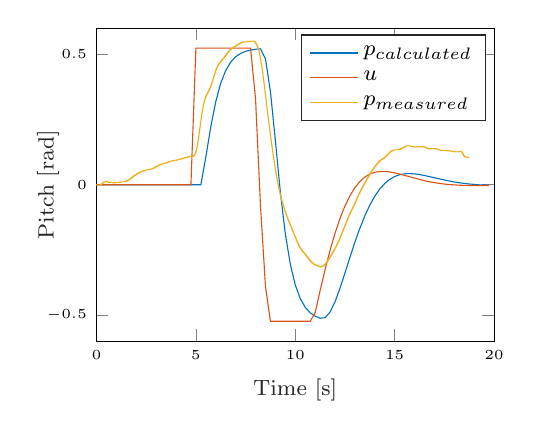
\begin{tikzpicture}

\begin{axis}[%
width=5.05cm,
height=3.975cm,
at={(0cm,0cm)},
scale only axis,
xmin=0,
xmax=20,
xlabel style={font=\color{white!15!black}},
xlabel={\footnotesize{Time [s]}},
ymin=-0.6,
ymax=0.6,
ylabel style={font=\color{white!15!black}},
ylabel={\footnotesize{Pitch [rad]}},
ylabel shift = -0.4cm,
ticklabel style = {font = \tiny},
axis background/.style={fill=white},
legend style={legend cell align=left, align=left, draw=white!15!black, font = \footnotesize}
]
\addplot [color=mycolor1]
  table[row sep=crcr]{%
0	0\\
5.25	0\\
5.5	0.106028752059022\\
5.75	0.22266037932344\\
6	0.318881471816436\\
6.25	0.389443606311282\\
6.5	0.437955073776589\\
6.75	0.469972642303759\\
7	0.490517248775326\\
7.25	0.503431001414494\\
7.5	0.51142138586015\\
7.75	0.516304398576697\\
8	0.51925862126776\\
8.25	0.521031154883602\\
8.5	0.482810924489247\\
8.75	0.356835413424932\\
9	0.167461036201846\\
9.25	-0.029764323976778\\
9.5	-0.189426471823346\\
9.75	-0.305394163031721\\
10	-0.38466082364566\\
10.25	-0.436773923734016\\
10.5	-0.470120168998651\\
10.75	-0.491036826023787\\
11	-0.503957909562715\\
11.25	-0.511843812705287\\
11.5	-0.509873884142213\\
11.75	-0.488044662546461\\
12	-0.448317562621909\\
12.25	-0.396302164538795\\
12.5	-0.337841222779961\\
12.75	-0.277797273112583\\
13	-0.219777579686458\\
13.25	-0.166223560264768\\
13.5	-0.118614773398843\\
13.75	-0.0776857142937644\\
14	-0.0436189313642856\\
14.25	-0.0162051508067833\\
14.5	0.00502861402445376\\
14.75	0.0207188048747398\\
15	0.031588306158298\\
15.25	0.0383885280986647\\
15.5	0.0418570731669057\\
15.75	0.042688053272844\\
16	0.0415125969082375\\
16.25	0.0388874620685478\\
16.5	0.035289978489164\\
17	0.0266922100468285\\
17.5	0.0180198945219239\\
18	0.010566875368891\\
18.25	0.00748975446615319\\
18.75	0.00272129828724843\\
19.25	-0.000331544740699741\\
19.75	-0.00198440960987156\\
};
\addlegendentry{$p_{\text{calculated}}$}

\addplot [color=mycolor2]
  table[row sep=crcr]{%
0	0\\
4.75	0\\
5	0.523598775599787\\
7.75	0.52359877559762\\
8	0.329641417534724\\
8.25	-0.0821959464738349\\
8.5	-0.390161056333724\\
8.75	-0.523598771544535\\
10.75	-0.523598775597524\\
11	-0.490335594119092\\
11.25	-0.405017991769771\\
11.5	-0.324470537154674\\
11.75	-0.250796820123448\\
12	-0.185308170273647\\
12.25	-0.128658433716605\\
12.5	-0.0809755513755839\\
12.75	-0.0419846801294881\\
13	-0.0111188887049423\\
13.25	0.0123847380981346\\
13.5	0.0294043723738433\\
13.75	0.040867877136133\\
14	0.0477014971566447\\
14.25	0.0507914633520414\\
14.5	0.0509569211776757\\
14.75	0.0489324928353057\\
15	0.0453587894876932\\
15.25	0.0407792717979873\\
16.5	0.0154955264225727\\
16.75	0.0114346776197891\\
17	0.00792142596289125\\
17.25	0.00496501724260767\\
17.5	0.00254888290762523\\
17.75	0.000637883187366128\\
18.25	-0.00186603813065389\\
18.75	-0.00298985344670655\\
19.25	-0.00318120213370676\\
19.75	-0.00282514330664796\\
};
\addlegendentry{$u$}

\addplot [color=mycolor3]
  table[row sep=crcr]{%
0	0\\
0.00799999999999912	0\\
0.0100000000000016	-0.00153398078788669\\
0.0599999999999987	-0.00153398078788669\\
0.0620000000000012	-0.00306796157576983\\
0.123999999999999	-0.00306796157576983\\
0.126000000000001	-0.00153398078788669\\
0.193999999999999	-0.00153398078788669\\
0.196000000000002	0\\
0.23	0\\
0.231999999999999	0.00153398078788669\\
0.260000000000002	0.00153398078788669\\
0.262	0.00306796157576983\\
0.283999999999999	0.00306796157576983\\
0.286000000000001	0.00460194236365652\\
0.303999999999998	0.00460194236365652\\
0.306000000000001	0.00613592315154321\\
0.334	0.00613592315154321\\
0.335999999999999	0.0076699039394299\\
0.350000000000001	0.0076699039394299\\
0.352	0.00920388472731304\\
0.382000000000001	0.00920388472731304\\
0.384	0.0107378655151997\\
0.446000000000002	0.0107378655151997\\
0.448	0.0122718463030864\\
0.530000000000001	0.0122718463030864\\
0.532	0.0107378655151997\\
0.597999999999999	0.0107378655151997\\
0.600000000000001	0.00920388472731304\\
0.82	0.00920388472731304\\
0.821999999999999	0.0076699039394299\\
0.960000000000001	0.0076699039394299\\
0.962	0.00920388472731304\\
1.21	0.00920388472731304\\
1.212	0.0107378655151997\\
1.396	0.0107378655151997\\
1.398	0.0122718463030864\\
1.482	0.0122718463030864\\
1.484	0.0138058270909696\\
1.53	0.0138058270909696\\
1.532	0.0153398078788562\\
1.572	0.0153398078788562\\
1.574	0.0168737886667429\\
1.608	0.0168737886667429\\
1.61	0.0184077694546261\\
1.636	0.0184077694546261\\
1.638	0.0199417502425128\\
1.668	0.0199417502425128\\
1.67	0.0214757310303995\\
1.694	0.0214757310303995\\
1.696	0.0230097118182861\\
1.72	0.0230097118182861\\
1.722	0.0245436926061693\\
1.748	0.0245436926061693\\
1.75	0.026077673394056\\
1.774	0.026077673394056\\
1.776	0.0276116541819427\\
1.798	0.0276116541819427\\
1.8	0.0291456349698258\\
1.82	0.0291456349698258\\
1.822	0.0306796157577125\\
1.848	0.0306796157577125\\
1.85	0.0322135965455992\\
1.872	0.0322135965455992\\
1.874	0.0337475773334859\\
1.9	0.0337475773334859\\
1.902	0.035281558121369\\
1.93	0.035281558121369\\
1.932	0.0368155389092557\\
1.96	0.0368155389092557\\
1.962	0.0383495196971424\\
1.99	0.0383495196971424\\
1.992	0.0398835004850255\\
2.022	0.0398835004850255\\
2.024	0.0414174812729122\\
2.054	0.0414174812729122\\
2.056	0.0429514620607989\\
2.092	0.0429514620607989\\
2.094	0.0444854428486821\\
2.128	0.0444854428486821\\
2.13	0.0460194236365687\\
2.164	0.0460194236365687\\
2.166	0.0475534044244554\\
2.208	0.0475534044244554\\
2.21	0.0490873852123421\\
2.25	0.0490873852123421\\
2.252	0.0506213660002253\\
2.296	0.0506213660002253\\
2.298	0.052155346788112\\
2.356	0.052155346788112\\
2.358	0.0536893275759986\\
2.418	0.0536893275759986\\
2.42	0.0552233083638818\\
2.488	0.0552233083638818\\
2.49	0.0567572891517685\\
2.596	0.0567572891517685\\
2.598	0.0582912699396552\\
2.71	0.0582912699396552\\
2.712	0.0598252507275383\\
2.782	0.0598252507275383\\
2.784	0.061359231515425\\
2.83	0.061359231515425\\
2.832	0.0628932123033117\\
2.872	0.0628932123033117\\
2.874	0.0644271930911984\\
2.91	0.0644271930911984\\
2.912	0.0659611738790815\\
2.948	0.0659611738790815\\
2.95	0.0674951546669682\\
2.986	0.0674951546669682\\
2.988	0.0690291354548549\\
3.026	0.0690291354548549\\
3.028	0.070563116242738\\
3.058	0.070563116242738\\
3.06	0.0720970970306247\\
3.092	0.0720970970306247\\
3.094	0.0736310778185114\\
3.134	0.0736310778185114\\
3.136	0.0751650586063981\\
3.174	0.0751650586063981\\
3.176	0.0766990393942812\\
3.228	0.0766990393942812\\
3.23	0.0782330201821679\\
3.288	0.0782330201821679\\
3.29	0.0797670009700546\\
3.366	0.0797670009700546\\
3.368	0.0813009817579378\\
3.444	0.0813009817579378\\
3.446	0.0828349625458245\\
3.504	0.0828349625458245\\
3.506	0.0843689433337111\\
3.558	0.0843689433337111\\
3.56	0.0859029241215943\\
3.608	0.0859029241215943\\
3.61	0.087436904909481\\
3.664	0.087436904909481\\
3.666	0.0889708856973677\\
3.728	0.0889708856973677\\
3.73	0.0905048664852544\\
3.806	0.0905048664852544\\
3.808	0.0920388472731375\\
3.912	0.0920388472731375\\
3.914	0.0935728280610242\\
4.022	0.0935728280610242\\
4.024	0.0951068088489109\\
4.104	0.0951068088489109\\
4.106	0.096640789636794\\
4.176	0.096640789636794\\
4.178	0.0981747704246807\\
4.254	0.0981747704246807\\
4.256	0.0997087512125674\\
4.326	0.0997087512125674\\
4.328	0.101242732000454\\
4.41	0.101242732000454\\
4.412	0.102776712788337\\
4.472	0.102776712788337\\
4.474	0.104310693576224\\
4.534	0.104310693576224\\
4.536	0.105844674364111\\
4.594	0.105844674364111\\
4.596	0.107378655151994\\
4.686	0.107378655151994\\
4.688	0.10891263593988\\
4.886	0.10891263593988\\
4.888	0.110446616727767\\
4.912	0.110446616727767\\
4.914	0.11198059751565\\
4.928	0.11198059751565\\
4.93	0.113514578303537\\
4.94	0.113514578303537\\
4.942	0.115048559091424\\
4.95	0.115048559091424\\
4.952	0.11658253987931\\
4.962	0.11658253987931\\
4.964	0.118116520667193\\
4.97	0.118116520667193\\
4.972	0.11965050145508\\
4.978	0.11965050145508\\
4.98	0.121184482242967\\
4.984	0.121184482242967\\
4.986	0.12271846303085\\
4.992	0.12271846303085\\
4.994	0.124252443818737\\
4.998	0.124252443818737\\
5	0.125786424606623\\
5.004	0.125786424606623\\
5.006	0.127320405394507\\
5.01	0.127320405394507\\
5.012	0.128854386182393\\
5.016	0.128854386182393\\
5.018	0.13038836697028\\
5.02	0.13038836697028\\
5.022	0.131922347758167\\
5.026	0.131922347758167\\
5.028	0.13345632854605\\
5.03	0.13345632854605\\
5.032	0.134990309333936\\
5.034	0.134990309333936\\
5.036	0.136524290121823\\
5.04	0.136524290121823\\
5.042	0.138058270909706\\
5.044	0.138058270909706\\
5.046	0.139592251697593\\
5.048	0.139592251697593\\
5.05	0.14112623248548\\
5.052	0.14112623248548\\
5.054	0.142660213273366\\
5.056	0.142660213273366\\
5.058	0.144194194061249\\
5.06	0.144194194061249\\
5.062	0.145728174849136\\
5.064	0.145728174849136\\
5.066	0.147262155637023\\
5.068	0.147262155637023\\
5.07	0.148796136424906\\
5.072	0.148796136424906\\
5.076	0.151864098000679\\
5.078	0.151864098000679\\
5.08	0.153398078788562\\
5.082	0.153398078788562\\
5.084	0.154932059576449\\
5.086	0.154932059576449\\
5.088	0.156466040364336\\
5.09	0.156466040364336\\
5.094	0.159534001940106\\
5.096	0.159534001940106\\
5.1	0.162601963515879\\
5.102	0.162601963515879\\
5.104	0.164135944303762\\
5.106	0.164135944303762\\
5.11	0.167203905879536\\
5.112	0.167203905879536\\
5.116	0.170271867455305\\
5.118	0.170271867455305\\
5.122	0.173339829031079\\
5.124	0.173339829031079\\
5.128	0.176407790606849\\
5.13	0.176407790606849\\
5.134	0.179475752182618\\
5.136	0.179475752182618\\
5.14	0.182543713758392\\
5.142	0.182543713758392\\
5.146	0.185611675334162\\
5.148	0.185611675334162\\
5.154	0.190213617697818\\
5.156	0.190213617697818\\
5.162	0.194815560061475\\
5.164	0.194815560061475\\
5.168	0.197883521637248\\
5.17	0.197883521637248\\
5.176	0.202485464000905\\
5.178	0.202485464000905\\
5.182	0.205553425576674\\
5.184	0.205553425576674\\
5.192	0.211689348728218\\
5.194	0.211689348728218\\
5.198	0.214757310303991\\
5.2	0.214757310303991\\
5.208	0.220893233455531\\
5.21	0.220893233455531\\
5.214	0.223961195031304\\
5.216	0.223961195031304\\
5.222	0.228563137394961\\
5.224	0.228563137394961\\
5.23	0.233165079758617\\
5.232	0.233165079758617\\
5.238	0.237767022122274\\
5.24	0.237767022122274\\
5.244	0.240834983698047\\
5.246	0.240834983698047\\
5.252	0.245436926061704\\
5.254	0.245436926061704\\
5.26	0.25003886842536\\
5.262	0.25003886842536\\
5.264	0.251572849213247\\
5.266	0.251572849213247\\
5.274	0.257708772364786\\
5.276	0.257708772364786\\
5.278	0.259242753152673\\
5.28	0.259242753152673\\
5.286	0.26384469551633\\
5.288	0.26384469551633\\
5.292	0.266912657092103\\
5.294	0.266912657092103\\
5.296	0.268446637879986\\
5.298	0.268446637879986\\
5.302	0.27151459945576\\
5.304	0.27151459945576\\
5.308	0.274582561031529\\
5.31	0.274582561031529\\
5.312	0.276116541819416\\
5.314	0.276116541819416\\
5.318	0.279184503395186\\
5.32	0.279184503395186\\
5.324	0.282252464970959\\
5.326	0.282252464970959\\
5.328	0.283786445758842\\
5.33	0.283786445758842\\
5.332	0.285320426546729\\
5.334	0.285320426546729\\
5.338	0.288388388122499\\
5.34	0.288388388122499\\
5.342	0.289922368910386\\
5.344	0.289922368910386\\
5.346	0.291456349698272\\
5.348	0.291456349698272\\
5.35	0.292990330486159\\
5.352	0.292990330486159\\
5.354	0.294524311274042\\
5.356	0.294524311274042\\
5.358	0.296058292061929\\
5.36	0.296058292061929\\
5.362	0.297592272849815\\
5.364	0.297592272849815\\
5.368	0.300660234425585\\
5.37	0.300660234425585\\
5.372	0.302194215213472\\
5.376	0.302194215213472\\
5.378	0.303728196001359\\
5.38	0.303728196001359\\
5.384	0.306796157577129\\
5.388	0.306796157577129\\
5.39	0.308330138365015\\
5.392	0.308330138365015\\
5.394	0.309864119152898\\
5.396	0.309864119152898\\
5.398	0.311398099940785\\
5.4	0.311398099940785\\
5.402	0.312932080728672\\
5.408	0.312932080728672\\
5.412	0.316000042304442\\
5.416	0.316000042304442\\
5.418	0.317534023092328\\
5.422	0.317534023092328\\
5.424	0.319068003880215\\
5.426	0.319068003880215\\
5.428	0.320601984668098\\
5.432	0.320601984668098\\
5.434	0.322135965455985\\
5.438	0.322135965455985\\
5.44	0.323669946243871\\
5.444	0.323669946243871\\
5.446	0.325203927031755\\
5.448	0.325203927031755\\
5.45	0.326737907819641\\
5.456	0.326737907819641\\
5.458	0.328271888607528\\
5.462	0.328271888607528\\
5.464	0.329805869395411\\
5.468	0.329805869395411\\
5.47	0.331339850183298\\
5.476	0.331339850183298\\
5.478	0.332873830971185\\
5.482	0.332873830971185\\
5.484	0.334407811759071\\
5.49	0.334407811759071\\
5.492	0.335941792546954\\
5.496	0.335941792546954\\
5.498	0.337475773334841\\
5.506	0.337475773334841\\
5.508	0.339009754122728\\
5.514	0.339009754122728\\
5.516	0.340543734910611\\
5.522	0.340543734910611\\
5.524	0.342077715698498\\
5.534	0.342077715698498\\
5.536	0.343611696486384\\
5.542	0.343611696486384\\
5.544	0.345145677274271\\
5.552	0.345145677274271\\
5.554	0.346679658062154\\
5.564	0.346679658062154\\
5.566	0.348213638850041\\
5.572	0.348213638850041\\
5.574	0.349747619637927\\
5.584	0.349747619637927\\
5.586	0.351281600425811\\
5.594	0.351281600425811\\
5.596	0.352815581213697\\
5.604	0.352815581213697\\
5.606	0.354349562001584\\
5.616	0.354349562001584\\
5.618	0.355883542789467\\
5.626	0.355883542789467\\
5.628	0.357417523577354\\
5.636	0.357417523577354\\
5.638	0.35895150436524\\
5.646	0.35895150436524\\
5.648	0.360485485153127\\
5.656	0.360485485153127\\
5.658	0.36201946594101\\
5.666	0.36201946594101\\
5.668	0.363553446728897\\
5.676	0.363553446728897\\
5.678	0.365087427516784\\
5.684	0.365087427516784\\
5.686	0.366621408304667\\
5.694	0.366621408304667\\
5.696	0.368155389092554\\
5.702	0.368155389092554\\
5.704	0.36968936988044\\
5.712	0.36968936988044\\
5.714	0.371223350668327\\
5.718	0.371223350668327\\
5.72	0.37275733145621\\
5.728	0.37275733145621\\
5.73	0.374291312244097\\
5.734	0.374291312244097\\
5.736	0.375825293031983\\
5.742	0.375825293031983\\
5.744	0.377359273819867\\
5.75	0.377359273819867\\
5.752	0.378893254607753\\
5.758	0.378893254607753\\
5.76	0.38042723539564\\
5.766	0.38042723539564\\
5.768	0.381961216183523\\
5.772	0.381961216183523\\
5.774	0.38349519697141\\
5.778	0.38349519697141\\
5.78	0.385029177759296\\
5.784	0.385029177759296\\
5.786	0.386563158547183\\
5.792	0.386563158547183\\
5.794	0.388097139335066\\
5.798	0.388097139335066\\
5.8	0.389631120122953\\
5.806	0.389631120122953\\
5.808	0.39116510091084\\
5.812	0.39116510091084\\
5.814	0.392699081698723\\
5.818	0.392699081698723\\
5.82	0.394233062486609\\
5.826	0.394233062486609\\
5.828	0.395767043274496\\
5.83	0.395767043274496\\
5.832	0.397301024062379\\
5.838	0.397301024062379\\
5.84	0.398835004850266\\
5.844	0.398835004850266\\
5.846	0.400368985638153\\
5.85	0.400368985638153\\
5.852	0.401902966426039\\
5.856	0.401902966426039\\
5.858	0.403436947213923\\
5.862	0.403436947213923\\
5.864	0.404970928001809\\
5.868	0.404970928001809\\
5.87	0.406504908789696\\
5.874	0.406504908789696\\
5.876	0.408038889577579\\
5.88	0.408038889577579\\
5.882	0.409572870365466\\
5.886	0.409572870365466\\
5.888	0.411106851153352\\
5.892	0.411106851153352\\
5.894	0.412640831941239\\
5.898	0.412640831941239\\
5.9	0.414174812729122\\
5.904	0.414174812729122\\
5.906	0.415708793517009\\
5.91	0.415708793517009\\
5.912	0.417242774304896\\
5.916	0.417242774304896\\
5.918	0.418776755092779\\
5.922	0.418776755092779\\
5.924	0.420310735880665\\
5.928	0.420310735880665\\
5.93	0.421844716668552\\
5.936	0.421844716668552\\
5.938	0.423378697456435\\
5.942	0.423378697456435\\
5.944	0.424912678244322\\
5.948	0.424912678244322\\
5.95	0.426446659032209\\
5.956	0.426446659032209\\
5.958	0.427980639820095\\
5.96	0.427980639820095\\
5.962	0.429514620607979\\
5.968	0.429514620607979\\
5.97	0.431048601395865\\
5.974	0.431048601395865\\
5.976	0.432582582183752\\
5.982	0.432582582183752\\
5.984	0.434116562971635\\
5.988	0.434116562971635\\
5.99	0.435650543759522\\
5.996	0.435650543759522\\
5.998	0.437184524547408\\
6.002	0.437184524547408\\
6.004	0.438718505335295\\
6.01	0.438718505335295\\
6.012	0.440252486123178\\
6.018	0.440252486123178\\
6.02	0.441786466911065\\
6.024	0.441786466911065\\
6.026	0.443320447698952\\
6.034	0.443320447698952\\
6.036	0.444854428486835\\
6.042	0.444854428486835\\
6.044	0.446388409274721\\
6.048	0.446388409274721\\
6.05	0.447922390062608\\
6.06	0.447922390062608\\
6.062	0.449456370850491\\
6.066	0.449456370850491\\
6.068	0.450990351638378\\
6.076	0.450990351638378\\
6.078	0.452524332426265\\
6.088	0.452524332426265\\
6.09	0.454058313214151\\
6.096	0.454058313214151\\
6.098	0.455592294002034\\
6.106	0.455592294002034\\
6.108	0.457126274789921\\
6.12	0.457126274789921\\
6.122	0.458660255577808\\
6.132	0.458660255577808\\
6.134	0.460194236365691\\
6.144	0.460194236365691\\
6.146	0.461728217153578\\
6.156	0.461728217153578\\
6.158	0.463262197941464\\
6.17	0.463262197941464\\
6.172	0.464796178729351\\
6.182	0.464796178729351\\
6.184	0.466330159517234\\
6.202	0.466330159517234\\
6.204	0.467864140305121\\
6.218	0.467864140305121\\
6.22	0.469398121093008\\
6.234	0.469398121093008\\
6.236	0.470932101880891\\
6.248	0.470932101880891\\
6.25	0.472466082668777\\
6.264	0.472466082668777\\
6.266	0.474000063456664\\
6.282	0.474000063456664\\
6.284	0.475534044244547\\
6.304	0.475534044244547\\
6.306	0.477068025032434\\
6.318	0.477068025032434\\
6.32	0.478602005820321\\
6.334	0.478602005820321\\
6.336	0.480135986608207\\
6.35	0.480135986608207\\
6.352	0.48166996739609\\
6.366	0.48166996739609\\
6.368	0.483203948183977\\
6.38	0.483203948183977\\
6.382	0.484737928971864\\
6.402	0.484737928971864\\
6.404	0.486271909759747\\
6.416	0.486271909759747\\
6.418	0.487805890547634\\
6.432	0.487805890547634\\
6.434	0.48933987133552\\
6.446	0.48933987133552\\
6.448	0.490873852123404\\
6.46	0.490873852123404\\
6.462	0.49240783291129\\
6.474	0.49240783291129\\
6.476	0.493941813699177\\
6.488	0.493941813699177\\
6.49	0.495475794487064\\
6.502	0.495475794487064\\
6.504	0.497009775274947\\
6.518	0.497009775274947\\
6.52	0.498543756062833\\
6.532	0.498543756062833\\
6.534	0.50007773685072\\
6.546	0.50007773685072\\
6.548	0.501611717638603\\
6.56	0.501611717638603\\
6.562	0.50314569842649\\
6.578	0.50314569842649\\
6.58	0.504679679214377\\
6.596	0.504679679214377\\
6.598	0.506213660002263\\
6.612	0.506213660002263\\
6.614	0.507747640790146\\
6.628	0.507747640790146\\
6.63	0.509281621578033\\
6.644	0.509281621578033\\
6.646	0.51081560236592\\
6.66	0.51081560236592\\
6.662	0.512349583153803\\
6.684	0.512349583153803\\
6.686	0.51388356394169\\
6.7	0.51388356394169\\
6.702	0.515417544729576\\
6.726	0.515417544729576\\
6.728	0.516951525517459\\
6.744	0.516951525517459\\
6.746	0.518485506305346\\
6.77	0.518485506305346\\
6.772	0.520019487093233\\
6.788	0.520019487093233\\
6.79	0.52155346788112\\
6.816	0.52155346788112\\
6.818	0.523087448669003\\
6.842	0.523087448669003\\
6.844	0.524621429456889\\
6.87	0.524621429456889\\
6.872	0.526155410244776\\
6.9	0.526155410244776\\
6.902	0.527689391032659\\
6.928	0.527689391032659\\
6.93	0.529223371820546\\
6.962	0.529223371820546\\
6.964	0.530757352608433\\
6.994	0.530757352608433\\
6.996	0.532291333396319\\
7.022	0.532291333396319\\
7.024	0.533825314184202\\
7.052	0.533825314184202\\
7.054	0.535359294972089\\
7.092	0.535359294972089\\
7.094	0.536893275759976\\
7.124	0.536893275759976\\
7.126	0.538427256547859\\
7.154	0.538427256547859\\
7.156	0.539961237335746\\
7.192	0.539961237335746\\
7.194	0.541495218123632\\
7.23	0.541495218123632\\
7.232	0.543029198911515\\
7.276	0.543029198911515\\
7.278	0.544563179699402\\
7.32	0.544563179699402\\
7.322	0.546097160487289\\
7.404	0.546097160487289\\
7.406	0.547631141275176\\
7.514	0.547631141275176\\
7.516	0.549165122063059\\
7.766	0.549165122063059\\
7.768	0.550699102850945\\
7.91	0.550699102850945\\
7.912	0.549165122063059\\
7.952	0.549165122063059\\
7.954	0.547631141275176\\
7.972	0.547631141275176\\
7.974	0.546097160487289\\
7.994	0.546097160487289\\
7.996	0.544563179699402\\
8.008	0.544563179699402\\
8.01	0.543029198911515\\
8.022	0.543029198911515\\
8.024	0.541495218123632\\
8.036	0.541495218123632\\
8.038	0.539961237335746\\
8.046	0.539961237335746\\
8.048	0.538427256547859\\
8.056	0.538427256547859\\
8.058	0.536893275759976\\
8.068	0.536893275759976\\
8.07	0.535359294972089\\
8.074	0.535359294972089\\
8.076	0.533825314184202\\
8.084	0.533825314184202\\
8.086	0.532291333396319\\
8.092	0.532291333396319\\
8.094	0.530757352608433\\
8.098	0.530757352608433\\
8.1	0.529223371820546\\
8.106	0.529223371820546\\
8.108	0.527689391032659\\
8.114	0.527689391032659\\
8.116	0.526155410244776\\
8.12	0.526155410244776\\
8.122	0.524621429456889\\
8.126	0.524621429456889\\
8.128	0.523087448669003\\
8.132	0.523087448669003\\
8.134	0.52155346788112\\
8.14	0.52155346788112\\
8.142	0.520019487093233\\
8.144	0.520019487093233\\
8.146	0.518485506305346\\
8.152	0.518485506305346\\
8.154	0.516951525517459\\
8.156	0.516951525517459\\
8.158	0.515417544729576\\
8.162	0.515417544729576\\
8.164	0.51388356394169\\
8.168	0.51388356394169\\
8.17	0.512349583153803\\
8.172	0.512349583153803\\
8.174	0.51081560236592\\
8.176	0.51081560236592\\
8.178	0.509281621578033\\
8.182	0.509281621578033\\
8.184	0.507747640790146\\
8.186	0.507747640790146\\
8.188	0.506213660002263\\
8.19	0.506213660002263\\
8.192	0.504679679214377\\
8.196	0.504679679214377\\
8.198	0.50314569842649\\
8.2	0.50314569842649\\
8.202	0.501611717638603\\
8.204	0.501611717638603\\
8.206	0.50007773685072\\
8.208	0.50007773685072\\
8.21	0.498543756062833\\
8.214	0.498543756062833\\
8.216	0.497009775274947\\
8.218	0.497009775274947\\
8.222	0.493941813699177\\
8.226	0.493941813699177\\
8.228	0.49240783291129\\
8.23	0.49240783291129\\
8.232	0.490873852123404\\
8.234	0.490873852123404\\
8.238	0.487805890547634\\
8.24	0.487805890547634\\
8.242	0.486271909759747\\
8.244	0.486271909759747\\
8.246	0.484737928971864\\
8.248	0.484737928971864\\
8.25	0.483203948183977\\
8.252	0.483203948183977\\
8.254	0.48166996739609\\
8.256	0.48166996739609\\
8.258	0.480135986608207\\
8.26	0.480135986608207\\
8.264	0.477068025032434\\
8.266	0.477068025032434\\
8.268	0.475534044244547\\
8.27	0.475534044244547\\
8.274	0.472466082668777\\
8.276	0.472466082668777\\
8.278	0.470932101880891\\
8.28	0.470932101880891\\
8.284	0.467864140305121\\
8.286	0.467864140305121\\
8.288	0.466330159517234\\
8.29	0.466330159517234\\
8.294	0.463262197941464\\
8.296	0.463262197941464\\
8.3	0.460194236365691\\
8.302	0.460194236365691\\
8.304	0.458660255577808\\
8.306	0.458660255577808\\
8.312	0.454058313214151\\
8.314	0.454058313214151\\
8.318	0.450990351638378\\
8.32	0.450990351638378\\
8.324	0.447922390062608\\
8.326	0.447922390062608\\
8.33	0.444854428486835\\
8.332	0.444854428486835\\
8.336	0.441786466911065\\
8.338	0.441786466911065\\
8.344	0.437184524547408\\
8.346	0.437184524547408\\
8.348	0.435650543759522\\
8.35	0.435650543759522\\
8.358	0.429514620607979\\
8.36	0.429514620607979\\
8.364	0.426446659032209\\
8.366	0.426446659032209\\
8.374	0.420310735880665\\
8.376	0.420310735880665\\
8.38	0.417242774304896\\
8.382	0.417242774304896\\
8.39	0.411106851153352\\
8.392	0.411106851153352\\
8.396	0.408038889577579\\
8.398	0.408038889577579\\
8.406	0.401902966426039\\
8.408	0.401902966426039\\
8.416	0.395767043274496\\
8.418	0.395767043274496\\
8.422	0.392699081698723\\
8.424	0.392699081698723\\
8.434	0.385029177759296\\
8.436	0.385029177759296\\
8.444	0.378893254607753\\
8.446	0.378893254607753\\
8.452	0.374291312244097\\
8.454	0.374291312244097\\
8.464	0.366621408304667\\
8.466	0.366621408304667\\
8.476	0.35895150436524\\
8.478	0.35895150436524\\
8.484	0.354349562001584\\
8.486	0.354349562001584\\
8.496	0.346679658062154\\
8.498	0.346679658062154\\
8.508	0.339009754122728\\
8.51	0.339009754122728\\
8.52	0.331339850183298\\
8.522	0.331339850183298\\
8.53	0.325203927031755\\
8.532	0.325203927031755\\
8.54	0.319068003880215\\
8.542	0.319068003880215\\
8.552	0.311398099940785\\
8.554	0.311398099940785\\
8.564	0.303728196001359\\
8.566	0.303728196001359\\
8.574	0.297592272849815\\
8.576	0.297592272849815\\
8.586	0.289922368910386\\
8.588	0.289922368910386\\
8.598	0.282252464970959\\
8.6	0.282252464970959\\
8.608	0.276116541819416\\
8.61	0.276116541819416\\
8.618	0.269980618667873\\
8.62	0.269980618667873\\
8.628	0.26384469551633\\
8.63	0.26384469551633\\
8.638	0.257708772364786\\
8.64	0.257708772364786\\
8.65	0.25003886842536\\
8.652	0.25003886842536\\
8.66	0.243902945273817\\
8.662	0.243902945273817\\
8.67	0.237767022122274\\
8.672	0.237767022122274\\
8.678	0.233165079758617\\
8.68	0.233165079758617\\
8.688	0.227029156607074\\
8.69	0.227029156607074\\
8.698	0.220893233455531\\
8.7	0.220893233455531\\
8.706	0.216291291091874\\
8.708	0.216291291091874\\
8.714	0.211689348728218\\
8.716	0.211689348728218\\
8.724	0.205553425576674\\
8.726	0.205553425576674\\
8.73	0.202485464000905\\
8.732	0.202485464000905\\
8.74	0.196349540849361\\
8.742	0.196349540849361\\
8.748	0.191747598485705\\
8.75	0.191747598485705\\
8.756	0.187145656122048\\
8.758	0.187145656122048\\
8.764	0.182543713758392\\
8.766	0.182543713758392\\
8.772	0.177941771394735\\
8.774	0.177941771394735\\
8.78	0.173339829031079\\
8.782	0.173339829031079\\
8.788	0.168737886667422\\
8.79	0.168737886667422\\
8.794	0.165669925091649\\
8.796	0.165669925091649\\
8.802	0.161067982727992\\
8.804	0.161067982727992\\
8.81	0.156466040364336\\
8.812	0.156466040364336\\
8.816	0.153398078788562\\
8.818	0.153398078788562\\
8.824	0.148796136424906\\
8.826	0.148796136424906\\
8.83	0.145728174849136\\
8.832	0.145728174849136\\
8.838	0.14112623248548\\
8.84	0.14112623248548\\
8.844	0.138058270909706\\
8.846	0.138058270909706\\
8.85	0.134990309333936\\
8.852	0.134990309333936\\
8.858	0.13038836697028\\
8.86	0.13038836697028\\
8.864	0.127320405394507\\
8.866	0.127320405394507\\
8.87	0.124252443818737\\
8.872	0.124252443818737\\
8.878	0.11965050145508\\
8.88	0.11965050145508\\
8.884	0.11658253987931\\
8.886	0.11658253987931\\
8.89	0.113514578303537\\
8.892	0.113514578303537\\
8.896	0.110446616727767\\
8.898	0.110446616727767\\
8.902	0.107378655151994\\
8.904	0.107378655151994\\
8.908	0.104310693576224\\
8.91	0.104310693576224\\
8.914	0.101242732000454\\
8.916	0.101242732000454\\
8.92	0.0981747704246807\\
8.922	0.0981747704246807\\
8.926	0.0951068088489109\\
8.928	0.0951068088489109\\
8.932	0.0920388472731375\\
8.934	0.0920388472731375\\
8.938	0.0889708856973677\\
8.94	0.0889708856973677\\
8.944	0.0859029241215943\\
8.946	0.0859029241215943\\
8.95	0.0828349625458245\\
8.952	0.0828349625458245\\
8.956	0.0797670009700546\\
8.958	0.0797670009700546\\
8.96	0.0782330201821679\\
8.962	0.0782330201821679\\
8.966	0.0751650586063981\\
8.968	0.0751650586063981\\
8.972	0.0720970970306247\\
8.974	0.0720970970306247\\
8.976	0.070563116242738\\
8.978	0.070563116242738\\
8.982	0.0674951546669682\\
8.984	0.0674951546669682\\
8.988	0.0644271930911984\\
8.99	0.0644271930911984\\
8.992	0.0628932123033117\\
8.994	0.0628932123033117\\
8.998	0.0598252507275383\\
9	0.0598252507275383\\
9.002	0.0582912699396552\\
9.004	0.0582912699396552\\
9.008	0.0552233083638818\\
9.01	0.0552233083638818\\
9.014	0.052155346788112\\
9.016	0.052155346788112\\
9.018	0.0506213660002253\\
9.02	0.0506213660002253\\
9.022	0.0490873852123421\\
9.024	0.0490873852123421\\
9.028	0.0460194236365687\\
9.03	0.0460194236365687\\
9.032	0.0444854428486821\\
9.034	0.0444854428486821\\
9.036	0.0429514620607989\\
9.038	0.0429514620607989\\
9.042	0.0398835004850255\\
9.044	0.0398835004850255\\
9.046	0.0383495196971424\\
9.048	0.0383495196971424\\
9.05	0.0368155389092557\\
9.052	0.0368155389092557\\
9.056	0.0337475773334859\\
9.058	0.0337475773334859\\
9.06	0.0322135965455992\\
9.062	0.0322135965455992\\
9.064	0.0306796157577125\\
9.066	0.0306796157577125\\
9.07	0.0276116541819427\\
9.072	0.0276116541819427\\
9.074	0.026077673394056\\
9.076	0.026077673394056\\
9.078	0.0245436926061693\\
9.08	0.0245436926061693\\
9.082	0.0230097118182861\\
9.084	0.0230097118182861\\
9.086	0.0214757310303995\\
9.088	0.0214757310303995\\
9.092	0.0184077694546261\\
9.094	0.0184077694546261\\
9.096	0.0168737886667429\\
9.098	0.0168737886667429\\
9.1	0.0153398078788562\\
9.102	0.0153398078788562\\
9.104	0.0138058270909696\\
9.106	0.0138058270909696\\
9.108	0.0122718463030864\\
9.11	0.0122718463030864\\
9.112	0.0107378655151997\\
9.114	0.0107378655151997\\
9.116	0.00920388472731304\\
9.118	0.00920388472731304\\
9.12	0.0076699039394299\\
9.122	0.0076699039394299\\
9.124	0.00613592315154321\\
9.126	0.00613592315154321\\
9.13	0.00306796157576983\\
9.134	0.00306796157576983\\
9.136	0.00153398078788669\\
9.138	0.00153398078788669\\
9.14	0\\
9.142	0\\
9.146	-0.00306796157576983\\
9.15	-0.00306796157576983\\
9.152	-0.00460194236365652\\
9.154	-0.00460194236365652\\
9.156	-0.00613592315154321\\
9.158	-0.00613592315154321\\
9.16	-0.0076699039394299\\
9.162	-0.0076699039394299\\
9.164	-0.00920388472731304\\
9.166	-0.00920388472731304\\
9.168	-0.0107378655151997\\
9.17	-0.0107378655151997\\
9.172	-0.0122718463030864\\
9.174	-0.0122718463030864\\
9.176	-0.0138058270909696\\
9.178	-0.0138058270909696\\
9.18	-0.0153398078788562\\
9.184	-0.0153398078788562\\
9.186	-0.0168737886667429\\
9.188	-0.0168737886667429\\
9.19	-0.0184077694546261\\
9.192	-0.0184077694546261\\
9.194	-0.0199417502425128\\
9.196	-0.0199417502425128\\
9.198	-0.0214757310303995\\
9.2	-0.0214757310303995\\
9.202	-0.0230097118182861\\
9.204	-0.0230097118182861\\
9.206	-0.0245436926061693\\
9.21	-0.0245436926061693\\
9.212	-0.026077673394056\\
9.214	-0.026077673394056\\
9.216	-0.0276116541819427\\
9.218	-0.0276116541819427\\
9.22	-0.0291456349698258\\
9.224	-0.0291456349698258\\
9.226	-0.0306796157577125\\
9.228	-0.0306796157577125\\
9.23	-0.0322135965455992\\
9.232	-0.0322135965455992\\
9.234	-0.0337475773334859\\
9.238	-0.0337475773334859\\
9.24	-0.035281558121369\\
9.242	-0.035281558121369\\
9.244	-0.0368155389092557\\
9.248	-0.0368155389092557\\
9.25	-0.0383495196971424\\
9.252	-0.0383495196971424\\
9.254	-0.0398835004850255\\
9.258	-0.0398835004850255\\
9.26	-0.0414174812729122\\
9.262	-0.0414174812729122\\
9.264	-0.0429514620607989\\
9.268	-0.0429514620607989\\
9.27	-0.0444854428486821\\
9.272	-0.0444854428486821\\
9.274	-0.0460194236365687\\
9.278	-0.0460194236365687\\
9.28	-0.0475534044244554\\
9.282	-0.0475534044244554\\
9.284	-0.0490873852123421\\
9.288	-0.0490873852123421\\
9.29	-0.0506213660002253\\
9.292	-0.0506213660002253\\
9.294	-0.052155346788112\\
9.298	-0.052155346788112\\
9.3	-0.0536893275759986\\
9.304	-0.0536893275759986\\
9.306	-0.0552233083638818\\
9.31	-0.0552233083638818\\
9.312	-0.0567572891517685\\
9.314	-0.0567572891517685\\
9.316	-0.0582912699396552\\
9.32	-0.0582912699396552\\
9.322	-0.0598252507275383\\
9.326	-0.0598252507275383\\
9.328	-0.061359231515425\\
9.33	-0.061359231515425\\
9.332	-0.0628932123033117\\
9.336	-0.0628932123033117\\
9.338	-0.0644271930911984\\
9.342	-0.0644271930911984\\
9.344	-0.0659611738790815\\
9.348	-0.0659611738790815\\
9.35	-0.0674951546669682\\
9.354	-0.0674951546669682\\
9.356	-0.0690291354548549\\
9.36	-0.0690291354548549\\
9.362	-0.070563116242738\\
9.366	-0.070563116242738\\
9.368	-0.0720970970306247\\
9.372	-0.0720970970306247\\
9.374	-0.0736310778185114\\
9.376	-0.0736310778185114\\
9.378	-0.0751650586063981\\
9.382	-0.0751650586063981\\
9.384	-0.0766990393942812\\
9.39	-0.0766990393942812\\
9.392	-0.0782330201821679\\
9.394	-0.0782330201821679\\
9.396	-0.0797670009700546\\
9.402	-0.0797670009700546\\
9.404	-0.0813009817579378\\
9.406	-0.0813009817579378\\
9.408	-0.0828349625458245\\
9.412	-0.0828349625458245\\
9.414	-0.0843689433337111\\
9.42	-0.0843689433337111\\
9.422	-0.0859029241215943\\
9.426	-0.0859029241215943\\
9.428	-0.087436904909481\\
9.432	-0.087436904909481\\
9.434	-0.0889708856973677\\
9.438	-0.0889708856973677\\
9.44	-0.0905048664852544\\
9.444	-0.0905048664852544\\
9.446	-0.0920388472731375\\
9.452	-0.0920388472731375\\
9.454	-0.0935728280610242\\
9.458	-0.0935728280610242\\
9.46	-0.0951068088489109\\
9.464	-0.0951068088489109\\
9.466	-0.096640789636794\\
9.47	-0.096640789636794\\
9.472	-0.0981747704246807\\
9.478	-0.0981747704246807\\
9.48	-0.0997087512125674\\
9.484	-0.0997087512125674\\
9.486	-0.101242732000454\\
9.49	-0.101242732000454\\
9.492	-0.102776712788337\\
9.498	-0.102776712788337\\
9.5	-0.104310693576224\\
9.504	-0.104310693576224\\
9.506	-0.105844674364111\\
9.512	-0.105844674364111\\
9.514	-0.107378655151994\\
9.518	-0.107378655151994\\
9.52	-0.10891263593988\\
9.526	-0.10891263593988\\
9.528	-0.110446616727767\\
9.532	-0.110446616727767\\
9.534	-0.11198059751565\\
9.54	-0.11198059751565\\
9.542	-0.113514578303537\\
9.546	-0.113514578303537\\
9.548	-0.115048559091424\\
9.554	-0.115048559091424\\
9.556	-0.11658253987931\\
9.562	-0.11658253987931\\
9.564	-0.118116520667193\\
9.57	-0.118116520667193\\
9.572	-0.11965050145508\\
9.576	-0.11965050145508\\
9.578	-0.121184482242967\\
9.584	-0.121184482242967\\
9.586	-0.12271846303085\\
9.592	-0.12271846303085\\
9.594	-0.124252443818737\\
9.598	-0.124252443818737\\
9.6	-0.125786424606623\\
9.606	-0.125786424606623\\
9.608	-0.127320405394507\\
9.614	-0.127320405394507\\
9.616	-0.128854386182393\\
9.622	-0.128854386182393\\
9.624	-0.13038836697028\\
9.63	-0.13038836697028\\
9.632	-0.131922347758167\\
9.638	-0.131922347758167\\
9.64	-0.13345632854605\\
9.644	-0.13345632854605\\
9.646	-0.134990309333936\\
9.654	-0.134990309333936\\
9.656	-0.136524290121823\\
9.66	-0.136524290121823\\
9.662	-0.138058270909706\\
9.668	-0.138058270909706\\
9.67	-0.139592251697593\\
9.676	-0.139592251697593\\
9.678	-0.14112623248548\\
9.684	-0.14112623248548\\
9.686	-0.142660213273366\\
9.692	-0.142660213273366\\
9.694	-0.144194194061249\\
9.7	-0.144194194061249\\
9.702	-0.145728174849136\\
9.708	-0.145728174849136\\
9.71	-0.147262155637023\\
9.716	-0.147262155637023\\
9.718	-0.148796136424906\\
9.724	-0.148796136424906\\
9.726	-0.150330117212793\\
9.732	-0.150330117212793\\
9.734	-0.151864098000679\\
9.74	-0.151864098000679\\
9.742	-0.153398078788562\\
9.748	-0.153398078788562\\
9.75	-0.154932059576449\\
9.756	-0.154932059576449\\
9.758	-0.156466040364336\\
9.764	-0.156466040364336\\
9.766	-0.158000021152223\\
9.772	-0.158000021152223\\
9.774	-0.159534001940106\\
9.78	-0.159534001940106\\
9.782	-0.161067982727992\\
9.788	-0.161067982727992\\
9.79	-0.162601963515879\\
9.798	-0.162601963515879\\
9.8	-0.164135944303762\\
9.806	-0.164135944303762\\
9.808	-0.165669925091649\\
9.814	-0.165669925091649\\
9.816	-0.167203905879536\\
9.822	-0.167203905879536\\
9.824	-0.168737886667422\\
9.832	-0.168737886667422\\
9.834	-0.170271867455305\\
9.84	-0.170271867455305\\
9.842	-0.171805848243192\\
9.848	-0.171805848243192\\
9.85	-0.173339829031079\\
9.856	-0.173339829031079\\
9.858	-0.174873809818962\\
9.864	-0.174873809818962\\
9.866	-0.176407790606849\\
9.872	-0.176407790606849\\
9.874	-0.177941771394735\\
9.882	-0.177941771394735\\
9.884	-0.179475752182618\\
9.89	-0.179475752182618\\
9.892	-0.181009732970505\\
9.898	-0.181009732970505\\
9.9	-0.182543713758392\\
9.906	-0.182543713758392\\
9.908	-0.184077694546279\\
9.914	-0.184077694546279\\
9.916	-0.185611675334162\\
9.922	-0.185611675334162\\
9.924	-0.187145656122048\\
9.932	-0.187145656122048\\
9.934	-0.188679636909935\\
9.94	-0.188679636909935\\
9.942	-0.190213617697818\\
9.948	-0.190213617697818\\
9.95	-0.191747598485705\\
9.956	-0.191747598485705\\
9.958	-0.193281579273592\\
9.964	-0.193281579273592\\
9.966	-0.194815560061475\\
9.972	-0.194815560061475\\
9.974	-0.196349540849361\\
9.98	-0.196349540849361\\
9.982	-0.197883521637248\\
9.988	-0.197883521637248\\
9.99	-0.199417502425135\\
9.996	-0.199417502425135\\
9.998	-0.200951483213018\\
10.006	-0.200951483213018\\
10.008	-0.202485464000905\\
10.014	-0.202485464000905\\
10.016	-0.204019444788791\\
10.022	-0.204019444788791\\
10.024	-0.205553425576674\\
10.03	-0.205553425576674\\
10.032	-0.207087406364561\\
10.038	-0.207087406364561\\
10.04	-0.208621387152448\\
10.048	-0.208621387152448\\
10.05	-0.210155367940335\\
10.056	-0.210155367940335\\
10.058	-0.211689348728218\\
10.064	-0.211689348728218\\
10.066	-0.213223329516104\\
10.072	-0.213223329516104\\
10.074	-0.214757310303991\\
10.08	-0.214757310303991\\
10.082	-0.216291291091874\\
10.088	-0.216291291091874\\
10.09	-0.217825271879761\\
10.098	-0.217825271879761\\
10.1	-0.219359252667648\\
10.106	-0.219359252667648\\
10.108	-0.220893233455531\\
10.116	-0.220893233455531\\
10.118	-0.222427214243417\\
10.124	-0.222427214243417\\
10.126	-0.223961195031304\\
10.132	-0.223961195031304\\
10.134	-0.225495175819191\\
10.142	-0.225495175819191\\
10.144	-0.227029156607074\\
10.152	-0.227029156607074\\
10.154	-0.228563137394961\\
10.16	-0.228563137394961\\
10.162	-0.230097118182847\\
10.17	-0.230097118182847\\
10.172	-0.23163109897073\\
10.18	-0.23163109897073\\
10.182	-0.233165079758617\\
10.19	-0.233165079758617\\
10.192	-0.234699060546504\\
10.2	-0.234699060546504\\
10.202	-0.23623304133439\\
10.21	-0.23623304133439\\
10.212	-0.237767022122274\\
10.222	-0.237767022122274\\
10.224	-0.23930100291016\\
10.232	-0.23930100291016\\
10.234	-0.240834983698047\\
10.244	-0.240834983698047\\
10.246	-0.24236896448593\\
10.256	-0.24236896448593\\
10.258	-0.243902945273817\\
10.266	-0.243902945273817\\
10.268	-0.245436926061704\\
10.282	-0.245436926061704\\
10.284	-0.246970906849587\\
10.294	-0.246970906849587\\
10.296	-0.248504887637473\\
10.308	-0.248504887637473\\
10.31	-0.25003886842536\\
10.322	-0.25003886842536\\
10.324	-0.251572849213247\\
10.338	-0.251572849213247\\
10.34	-0.25310683000113\\
10.354	-0.25310683000113\\
10.356	-0.254640810789017\\
10.37	-0.254640810789017\\
10.372	-0.256174791576903\\
10.386	-0.256174791576903\\
10.388	-0.257708772364786\\
10.406	-0.257708772364786\\
10.408	-0.259242753152673\\
10.424	-0.259242753152673\\
10.426	-0.26077673394056\\
10.442	-0.26077673394056\\
10.444	-0.262310714728443\\
10.458	-0.262310714728443\\
10.46	-0.26384469551633\\
10.48	-0.26384469551633\\
10.482	-0.265378676304216\\
10.496	-0.265378676304216\\
10.498	-0.266912657092103\\
10.512	-0.266912657092103\\
10.514	-0.268446637879986\\
10.528	-0.268446637879986\\
10.53	-0.269980618667873\\
10.544	-0.269980618667873\\
10.546	-0.27151459945576\\
10.558	-0.27151459945576\\
10.56	-0.273048580243643\\
10.574	-0.273048580243643\\
10.576	-0.274582561031529\\
10.59	-0.274582561031529\\
10.592	-0.276116541819416\\
10.61	-0.276116541819416\\
10.612	-0.277650522607303\\
10.622	-0.277650522607303\\
10.624	-0.279184503395186\\
10.64	-0.279184503395186\\
10.642	-0.280718484183073\\
10.654	-0.280718484183073\\
10.656	-0.282252464970959\\
10.67	-0.282252464970959\\
10.672	-0.283786445758842\\
10.686	-0.283786445758842\\
10.688	-0.285320426546729\\
10.7	-0.285320426546729\\
10.702	-0.286854407334616\\
10.716	-0.286854407334616\\
10.718	-0.288388388122499\\
10.734	-0.288388388122499\\
10.736	-0.289922368910386\\
10.752	-0.289922368910386\\
10.754	-0.291456349698272\\
10.77	-0.291456349698272\\
10.772	-0.292990330486159\\
10.786	-0.292990330486159\\
10.788	-0.294524311274042\\
10.806	-0.294524311274042\\
10.808	-0.296058292061929\\
10.826	-0.296058292061929\\
10.828	-0.297592272849815\\
10.844	-0.297592272849815\\
10.846	-0.299126253637699\\
10.868	-0.299126253637699\\
10.87	-0.300660234425585\\
10.894	-0.300660234425585\\
10.896	-0.302194215213472\\
10.916	-0.302194215213472\\
10.918	-0.303728196001359\\
10.95	-0.303728196001359\\
10.952	-0.305262176789242\\
10.984	-0.305262176789242\\
10.986	-0.306796157577129\\
11.026	-0.306796157577129\\
11.028	-0.308330138365015\\
11.068	-0.308330138365015\\
11.07	-0.309864119152898\\
11.122	-0.309864119152898\\
11.124	-0.311398099940785\\
11.17	-0.311398099940785\\
11.172	-0.312932080728672\\
11.258	-0.312932080728672\\
11.26	-0.314466061516555\\
11.308	-0.314466061516555\\
11.31	-0.312932080728672\\
11.376	-0.312932080728672\\
11.378	-0.311398099940785\\
11.406	-0.311398099940785\\
11.408	-0.309864119152898\\
11.436	-0.309864119152898\\
11.438	-0.308330138365015\\
11.46	-0.308330138365015\\
11.462	-0.306796157577129\\
11.482	-0.306796157577129\\
11.484	-0.305262176789242\\
11.502	-0.305262176789242\\
11.504	-0.303728196001359\\
11.52	-0.303728196001359\\
11.522	-0.302194215213472\\
11.538	-0.302194215213472\\
11.54	-0.300660234425585\\
11.554	-0.300660234425585\\
11.556	-0.299126253637699\\
11.568	-0.299126253637699\\
11.57	-0.297592272849815\\
11.584	-0.297592272849815\\
11.586	-0.296058292061929\\
11.6	-0.296058292061929\\
11.602	-0.294524311274042\\
11.614	-0.294524311274042\\
11.616	-0.292990330486159\\
11.628	-0.292990330486159\\
11.63	-0.291456349698272\\
11.642	-0.291456349698272\\
11.644	-0.289922368910386\\
11.654	-0.289922368910386\\
11.656	-0.288388388122499\\
11.668	-0.288388388122499\\
11.67	-0.286854407334616\\
11.682	-0.286854407334616\\
11.684	-0.285320426546729\\
11.694	-0.285320426546729\\
11.696	-0.283786445758842\\
11.706	-0.283786445758842\\
11.708	-0.282252464970959\\
11.718	-0.282252464970959\\
11.72	-0.280718484183073\\
11.73	-0.280718484183073\\
11.732	-0.279184503395186\\
11.744	-0.279184503395186\\
11.746	-0.277650522607303\\
11.756	-0.277650522607303\\
11.758	-0.276116541819416\\
11.768	-0.276116541819416\\
11.77	-0.274582561031529\\
11.78	-0.274582561031529\\
11.782	-0.273048580243643\\
11.79	-0.273048580243643\\
11.792	-0.27151459945576\\
11.802	-0.27151459945576\\
11.804	-0.269980618667873\\
11.814	-0.269980618667873\\
11.816	-0.268446637879986\\
11.828	-0.268446637879986\\
11.83	-0.266912657092103\\
11.84	-0.266912657092103\\
11.842	-0.265378676304216\\
11.85	-0.265378676304216\\
11.852	-0.26384469551633\\
11.86	-0.26384469551633\\
11.862	-0.262310714728443\\
11.872	-0.262310714728443\\
11.874	-0.26077673394056\\
11.884	-0.26077673394056\\
11.886	-0.259242753152673\\
11.896	-0.259242753152673\\
11.898	-0.257708772364786\\
11.906	-0.257708772364786\\
11.908	-0.256174791576903\\
11.918	-0.256174791576903\\
11.92	-0.254640810789017\\
11.93	-0.254640810789017\\
11.932	-0.25310683000113\\
11.94	-0.25310683000113\\
11.942	-0.251572849213247\\
11.952	-0.251572849213247\\
11.954	-0.25003886842536\\
11.962	-0.25003886842536\\
11.964	-0.248504887637473\\
11.972	-0.248504887637473\\
11.974	-0.246970906849587\\
11.984	-0.246970906849587\\
11.986	-0.245436926061704\\
11.994	-0.245436926061704\\
11.996	-0.243902945273817\\
12.004	-0.243902945273817\\
12.006	-0.24236896448593\\
12.016	-0.24236896448593\\
12.018	-0.240834983698047\\
12.028	-0.240834983698047\\
12.03	-0.23930100291016\\
12.038	-0.23930100291016\\
12.04	-0.237767022122274\\
12.048	-0.237767022122274\\
12.05	-0.23623304133439\\
12.06	-0.23623304133439\\
12.062	-0.234699060546504\\
12.068	-0.234699060546504\\
12.07	-0.233165079758617\\
12.078	-0.233165079758617\\
12.08	-0.23163109897073\\
12.09	-0.23163109897073\\
12.092	-0.230097118182847\\
12.1	-0.230097118182847\\
12.102	-0.228563137394961\\
12.108	-0.228563137394961\\
12.11	-0.227029156607074\\
12.118	-0.227029156607074\\
12.12	-0.225495175819191\\
12.128	-0.225495175819191\\
12.13	-0.223961195031304\\
12.138	-0.223961195031304\\
12.14	-0.222427214243417\\
12.146	-0.222427214243417\\
12.148	-0.220893233455531\\
12.156	-0.220893233455531\\
12.158	-0.219359252667648\\
12.166	-0.219359252667648\\
12.168	-0.217825271879761\\
12.174	-0.217825271879761\\
12.176	-0.216291291091874\\
12.182	-0.216291291091874\\
12.184	-0.214757310303991\\
12.192	-0.214757310303991\\
12.194	-0.213223329516104\\
12.202	-0.213223329516104\\
12.204	-0.211689348728218\\
12.21	-0.211689348728218\\
12.212	-0.210155367940335\\
12.22	-0.210155367940335\\
12.222	-0.208621387152448\\
12.228	-0.208621387152448\\
12.23	-0.207087406364561\\
12.236	-0.207087406364561\\
12.238	-0.205553425576674\\
12.246	-0.205553425576674\\
12.248	-0.204019444788791\\
12.254	-0.204019444788791\\
12.256	-0.202485464000905\\
12.262	-0.202485464000905\\
12.264	-0.200951483213018\\
12.27	-0.200951483213018\\
12.272	-0.199417502425135\\
12.28	-0.199417502425135\\
12.282	-0.197883521637248\\
12.288	-0.197883521637248\\
12.29	-0.196349540849361\\
12.296	-0.196349540849361\\
12.298	-0.194815560061475\\
12.304	-0.194815560061475\\
12.306	-0.193281579273592\\
12.314	-0.193281579273592\\
12.316	-0.191747598485705\\
12.322	-0.191747598485705\\
12.324	-0.190213617697818\\
12.33	-0.190213617697818\\
12.332	-0.188679636909935\\
12.338	-0.188679636909935\\
12.34	-0.187145656122048\\
12.346	-0.187145656122048\\
12.348	-0.185611675334162\\
12.354	-0.185611675334162\\
12.356	-0.184077694546279\\
12.362	-0.184077694546279\\
12.364	-0.182543713758392\\
12.37	-0.182543713758392\\
12.372	-0.181009732970505\\
12.378	-0.181009732970505\\
12.38	-0.179475752182618\\
12.386	-0.179475752182618\\
12.388	-0.177941771394735\\
12.394	-0.177941771394735\\
12.396	-0.176407790606849\\
12.402	-0.176407790606849\\
12.404	-0.174873809818962\\
12.41	-0.174873809818962\\
12.412	-0.173339829031079\\
12.418	-0.173339829031079\\
12.42	-0.171805848243192\\
12.426	-0.171805848243192\\
12.428	-0.170271867455305\\
12.434	-0.170271867455305\\
12.436	-0.168737886667422\\
12.442	-0.168737886667422\\
12.444	-0.167203905879536\\
12.448	-0.167203905879536\\
12.45	-0.165669925091649\\
12.458	-0.165669925091649\\
12.46	-0.164135944303762\\
12.466	-0.164135944303762\\
12.468	-0.162601963515879\\
12.474	-0.162601963515879\\
12.476	-0.161067982727992\\
12.48	-0.161067982727992\\
12.482	-0.159534001940106\\
12.49	-0.159534001940106\\
12.492	-0.158000021152223\\
12.498	-0.158000021152223\\
12.5	-0.156466040364336\\
12.506	-0.156466040364336\\
12.508	-0.154932059576449\\
12.514	-0.154932059576449\\
12.516	-0.153398078788562\\
12.522	-0.153398078788562\\
12.524	-0.151864098000679\\
12.53	-0.151864098000679\\
12.532	-0.150330117212793\\
12.538	-0.150330117212793\\
12.54	-0.148796136424906\\
12.544	-0.148796136424906\\
12.546	-0.147262155637023\\
12.552	-0.147262155637023\\
12.554	-0.145728174849136\\
12.562	-0.145728174849136\\
12.564	-0.144194194061249\\
12.57	-0.144194194061249\\
12.572	-0.142660213273366\\
12.578	-0.142660213273366\\
12.58	-0.14112623248548\\
12.586	-0.14112623248548\\
12.588	-0.139592251697593\\
12.594	-0.139592251697593\\
12.596	-0.138058270909706\\
12.602	-0.138058270909706\\
12.604	-0.136524290121823\\
12.61	-0.136524290121823\\
12.612	-0.134990309333936\\
12.62	-0.134990309333936\\
12.622	-0.13345632854605\\
12.628	-0.13345632854605\\
12.63	-0.131922347758167\\
12.636	-0.131922347758167\\
12.638	-0.13038836697028\\
12.644	-0.13038836697028\\
12.646	-0.128854386182393\\
12.654	-0.128854386182393\\
12.656	-0.127320405394507\\
12.662	-0.127320405394507\\
12.664	-0.125786424606623\\
12.672	-0.125786424606623\\
12.674	-0.124252443818737\\
12.68	-0.124252443818737\\
12.682	-0.12271846303085\\
12.69	-0.12271846303085\\
12.692	-0.121184482242967\\
12.698	-0.121184482242967\\
12.7	-0.11965050145508\\
12.706	-0.11965050145508\\
12.708	-0.118116520667193\\
12.716	-0.118116520667193\\
12.718	-0.11658253987931\\
12.724	-0.11658253987931\\
12.726	-0.115048559091424\\
12.734	-0.115048559091424\\
12.736	-0.113514578303537\\
12.742	-0.113514578303537\\
12.744	-0.11198059751565\\
12.752	-0.11198059751565\\
12.754	-0.110446616727767\\
12.762	-0.110446616727767\\
12.764	-0.10891263593988\\
12.77	-0.10891263593988\\
12.772	-0.107378655151994\\
12.78	-0.107378655151994\\
12.782	-0.105844674364111\\
12.79	-0.105844674364111\\
12.792	-0.104310693576224\\
12.798	-0.104310693576224\\
12.8	-0.102776712788337\\
12.808	-0.102776712788337\\
12.81	-0.101242732000454\\
12.818	-0.101242732000454\\
12.82	-0.0997087512125674\\
12.826	-0.0997087512125674\\
12.828	-0.0981747704246807\\
12.836	-0.0981747704246807\\
12.838	-0.096640789636794\\
12.846	-0.096640789636794\\
12.848	-0.0951068088489109\\
12.856	-0.0951068088489109\\
12.858	-0.0935728280610242\\
12.864	-0.0935728280610242\\
12.866	-0.0920388472731375\\
12.874	-0.0920388472731375\\
12.876	-0.0905048664852544\\
12.884	-0.0905048664852544\\
12.886	-0.0889708856973677\\
12.894	-0.0889708856973677\\
12.896	-0.087436904909481\\
12.902	-0.087436904909481\\
12.904	-0.0859029241215943\\
12.912	-0.0859029241215943\\
12.914	-0.0843689433337111\\
12.922	-0.0843689433337111\\
12.924	-0.0828349625458245\\
12.93	-0.0828349625458245\\
12.932	-0.0813009817579378\\
12.94	-0.0813009817579378\\
12.942	-0.0797670009700546\\
12.95	-0.0797670009700546\\
12.952	-0.0782330201821679\\
12.958	-0.0782330201821679\\
12.96	-0.0766990393942812\\
12.968	-0.0766990393942812\\
12.97	-0.0751650586063981\\
12.976	-0.0751650586063981\\
12.978	-0.0736310778185114\\
12.986	-0.0736310778185114\\
12.988	-0.0720970970306247\\
12.994	-0.0720970970306247\\
12.996	-0.070563116242738\\
13.004	-0.070563116242738\\
13.006	-0.0690291354548549\\
13.012	-0.0690291354548549\\
13.014	-0.0674951546669682\\
13.022	-0.0674951546669682\\
13.024	-0.0659611738790815\\
13.03	-0.0659611738790815\\
13.032	-0.0644271930911984\\
13.04	-0.0644271930911984\\
13.042	-0.0628932123033117\\
13.048	-0.0628932123033117\\
13.05	-0.061359231515425\\
13.058	-0.061359231515425\\
13.06	-0.0598252507275383\\
13.066	-0.0598252507275383\\
13.068	-0.0582912699396552\\
13.076	-0.0582912699396552\\
13.078	-0.0567572891517685\\
13.084	-0.0567572891517685\\
13.086	-0.0552233083638818\\
13.092	-0.0552233083638818\\
13.094	-0.0536893275759986\\
13.102	-0.0536893275759986\\
13.104	-0.052155346788112\\
13.112	-0.052155346788112\\
13.114	-0.0506213660002253\\
13.12	-0.0506213660002253\\
13.122	-0.0490873852123421\\
13.128	-0.0490873852123421\\
13.13	-0.0475534044244554\\
13.138	-0.0475534044244554\\
13.14	-0.0460194236365687\\
13.148	-0.0460194236365687\\
13.15	-0.0444854428486821\\
13.156	-0.0444854428486821\\
13.158	-0.0429514620607989\\
13.166	-0.0429514620607989\\
13.168	-0.0414174812729122\\
13.174	-0.0414174812729122\\
13.176	-0.0398835004850255\\
13.184	-0.0398835004850255\\
13.186	-0.0383495196971424\\
13.194	-0.0383495196971424\\
13.196	-0.0368155389092557\\
13.204	-0.0368155389092557\\
13.206	-0.035281558121369\\
13.214	-0.035281558121369\\
13.216	-0.0337475773334859\\
13.224	-0.0337475773334859\\
13.226	-0.0322135965455992\\
13.232	-0.0322135965455992\\
13.234	-0.0306796157577125\\
13.244	-0.0306796157577125\\
13.246	-0.0291456349698258\\
13.252	-0.0291456349698258\\
13.254	-0.0276116541819427\\
13.262	-0.0276116541819427\\
13.264	-0.026077673394056\\
13.272	-0.026077673394056\\
13.274	-0.0245436926061693\\
13.284	-0.0245436926061693\\
13.286	-0.0230097118182861\\
13.294	-0.0230097118182861\\
13.296	-0.0214757310303995\\
13.304	-0.0214757310303995\\
13.306	-0.0199417502425128\\
13.316	-0.0199417502425128\\
13.318	-0.0184077694546261\\
13.326	-0.0184077694546261\\
13.328	-0.0168737886667429\\
13.336	-0.0168737886667429\\
13.338	-0.0153398078788562\\
13.346	-0.0153398078788562\\
13.348	-0.0138058270909696\\
13.358	-0.0138058270909696\\
13.36	-0.0122718463030864\\
13.368	-0.0122718463030864\\
13.37	-0.0107378655151997\\
13.378	-0.0107378655151997\\
13.38	-0.00920388472731304\\
13.39	-0.00920388472731304\\
13.392	-0.0076699039394299\\
13.4	-0.0076699039394299\\
13.402	-0.00613592315154321\\
13.412	-0.00613592315154321\\
13.414	-0.00460194236365652\\
13.422	-0.00460194236365652\\
13.424	-0.00306796157576983\\
13.434	-0.00306796157576983\\
13.436	-0.00153398078788669\\
13.446	-0.00153398078788669\\
13.448	0\\
13.456	0\\
13.458	0.00153398078788669\\
13.468	0.00153398078788669\\
13.47	0.00306796157576983\\
13.48	0.00306796157576983\\
13.482	0.00460194236365652\\
13.492	0.00460194236365652\\
13.494	0.00613592315154321\\
13.502	0.00613592315154321\\
13.504	0.0076699039394299\\
13.514	0.0076699039394299\\
13.516	0.00920388472731304\\
13.526	0.00920388472731304\\
13.528	0.0107378655151997\\
13.536	0.0107378655151997\\
13.538	0.0122718463030864\\
13.548	0.0122718463030864\\
13.55	0.0138058270909696\\
13.558	0.0138058270909696\\
13.56	0.0153398078788562\\
13.57	0.0153398078788562\\
13.572	0.0168737886667429\\
13.582	0.0168737886667429\\
13.584	0.0184077694546261\\
13.594	0.0184077694546261\\
13.596	0.0199417502425128\\
13.604	0.0199417502425128\\
13.606	0.0214757310303995\\
13.616	0.0214757310303995\\
13.618	0.0230097118182861\\
13.626	0.0230097118182861\\
13.628	0.0245436926061693\\
13.638	0.0245436926061693\\
13.64	0.026077673394056\\
13.65	0.026077673394056\\
13.652	0.0276116541819427\\
13.66	0.0276116541819427\\
13.662	0.0291456349698258\\
13.672	0.0291456349698258\\
13.674	0.0306796157577125\\
13.684	0.0306796157577125\\
13.686	0.0322135965455992\\
13.696	0.0322135965455992\\
13.698	0.0337475773334859\\
13.708	0.0337475773334859\\
13.71	0.035281558121369\\
13.718	0.035281558121369\\
13.72	0.0368155389092557\\
13.732	0.0368155389092557\\
13.734	0.0383495196971424\\
13.744	0.0383495196971424\\
13.746	0.0398835004850255\\
13.756	0.0398835004850255\\
13.758	0.0414174812729122\\
13.768	0.0414174812729122\\
13.77	0.0429514620607989\\
13.782	0.0429514620607989\\
13.784	0.0444854428486821\\
13.794	0.0444854428486821\\
13.796	0.0460194236365687\\
13.806	0.0460194236365687\\
13.808	0.0475534044244554\\
13.818	0.0475534044244554\\
13.82	0.0490873852123421\\
13.832	0.0490873852123421\\
13.834	0.0506213660002253\\
13.844	0.0506213660002253\\
13.846	0.052155346788112\\
13.858	0.052155346788112\\
13.86	0.0536893275759986\\
13.872	0.0536893275759986\\
13.874	0.0552233083638818\\
13.884	0.0552233083638818\\
13.886	0.0567572891517685\\
13.898	0.0567572891517685\\
13.9	0.0582912699396552\\
13.912	0.0582912699396552\\
13.914	0.0598252507275383\\
13.926	0.0598252507275383\\
13.928	0.061359231515425\\
13.94	0.061359231515425\\
13.942	0.0628932123033117\\
13.952	0.0628932123033117\\
13.954	0.0644271930911984\\
13.966	0.0644271930911984\\
13.968	0.0659611738790815\\
13.978	0.0659611738790815\\
13.98	0.0674951546669682\\
13.992	0.0674951546669682\\
13.994	0.0690291354548549\\
14.006	0.0690291354548549\\
14.008	0.070563116242738\\
14.02	0.070563116242738\\
14.022	0.0720970970306247\\
14.034	0.0720970970306247\\
14.036	0.0736310778185114\\
14.05	0.0736310778185114\\
14.052	0.0751650586063981\\
14.064	0.0751650586063981\\
14.066	0.0766990393942812\\
14.08	0.0766990393942812\\
14.082	0.0782330201821679\\
14.096	0.0782330201821679\\
14.098	0.0797670009700546\\
14.112	0.0797670009700546\\
14.114	0.0813009817579378\\
14.132	0.0813009817579378\\
14.134	0.0828349625458245\\
14.148	0.0828349625458245\\
14.15	0.0843689433337111\\
14.166	0.0843689433337111\\
14.168	0.0859029241215943\\
14.186	0.0859029241215943\\
14.188	0.087436904909481\\
14.206	0.087436904909481\\
14.208	0.0889708856973677\\
14.23	0.0889708856973677\\
14.232	0.0905048664852544\\
14.25	0.0905048664852544\\
14.252	0.0920388472731375\\
14.278	0.0920388472731375\\
14.28	0.0935728280610242\\
14.306	0.0935728280610242\\
14.308	0.0951068088489109\\
14.336	0.0951068088489109\\
14.338	0.096640789636794\\
14.366	0.096640789636794\\
14.368	0.0981747704246807\\
14.4	0.0981747704246807\\
14.402	0.0997087512125674\\
14.43	0.0997087512125674\\
14.432	0.101242732000454\\
14.458	0.101242732000454\\
14.46	0.102776712788337\\
14.484	0.102776712788337\\
14.486	0.104310693576224\\
14.508	0.104310693576224\\
14.51	0.105844674364111\\
14.53	0.105844674364111\\
14.532	0.107378655151994\\
14.552	0.107378655151994\\
14.554	0.10891263593988\\
14.572	0.10891263593988\\
14.574	0.110446616727767\\
14.594	0.110446616727767\\
14.596	0.11198059751565\\
14.614	0.11198059751565\\
14.616	0.113514578303537\\
14.634	0.113514578303537\\
14.636	0.115048559091424\\
14.652	0.115048559091424\\
14.654	0.11658253987931\\
14.674	0.11658253987931\\
14.676	0.118116520667193\\
14.692	0.118116520667193\\
14.694	0.11965050145508\\
14.712	0.11965050145508\\
14.714	0.121184482242967\\
14.73	0.121184482242967\\
14.732	0.12271846303085\\
14.752	0.12271846303085\\
14.754	0.124252443818737\\
14.772	0.124252443818737\\
14.774	0.125786424606623\\
14.798	0.125786424606623\\
14.8	0.127320405394507\\
14.824	0.127320405394507\\
14.826	0.128854386182393\\
14.854	0.128854386182393\\
14.856	0.13038836697028\\
14.888	0.13038836697028\\
14.89	0.131922347758167\\
14.942	0.131922347758167\\
14.944	0.13345632854605\\
15.158	0.13345632854605\\
15.16	0.134990309333936\\
15.254	0.134990309333936\\
15.256	0.136524290121823\\
15.3	0.136524290121823\\
15.302	0.138058270909706\\
15.342	0.138058270909706\\
15.344	0.139592251697593\\
15.374	0.139592251697593\\
15.376	0.14112623248548\\
15.414	0.14112623248548\\
15.416	0.142660213273366\\
15.448	0.142660213273366\\
15.45	0.144194194061249\\
15.492	0.144194194061249\\
15.494	0.145728174849136\\
15.536	0.145728174849136\\
15.538	0.147262155637023\\
15.596	0.147262155637023\\
15.598	0.148796136424906\\
15.808	0.148796136424906\\
15.81	0.147262155637023\\
15.898	0.147262155637023\\
15.9	0.145728174849136\\
16.002	0.145728174849136\\
16.004	0.144194194061249\\
16.112	0.144194194061249\\
16.114	0.145728174849136\\
16.302	0.145728174849136\\
16.304	0.147262155637023\\
16.386	0.147262155637023\\
16.388	0.145728174849136\\
16.472	0.145728174849136\\
16.474	0.144194194061249\\
16.53	0.144194194061249\\
16.532	0.142660213273366\\
16.578	0.142660213273366\\
16.58	0.14112623248548\\
16.644	0.14112623248548\\
16.646	0.139592251697593\\
16.72	0.139592251697593\\
16.722	0.138058270909706\\
16.858	0.138058270909706\\
16.86	0.139592251697593\\
17.016	0.139592251697593\\
17.018	0.138058270909706\\
17.094	0.138058270909706\\
17.096	0.136524290121823\\
17.148	0.136524290121823\\
17.15	0.134990309333936\\
17.208	0.134990309333936\\
17.21	0.13345632854605\\
17.278	0.13345632854605\\
17.28	0.131922347758167\\
17.598	0.131922347758167\\
17.6	0.13038836697028\\
17.77	0.13038836697028\\
17.772	0.128854386182393\\
17.904	0.128854386182393\\
17.906	0.127320405394507\\
18.04	0.127320405394507\\
18.042	0.125786424606623\\
18.19	0.125786424606623\\
18.192	0.127320405394507\\
18.36	0.127320405394507\\
18.362	0.125786424606623\\
18.378	0.125786424606623\\
18.38	0.124252443818737\\
18.39	0.124252443818737\\
18.392	0.12271846303085\\
18.404	0.12271846303085\\
18.406	0.121184482242967\\
18.412	0.121184482242967\\
18.414	0.11965050145508\\
18.424	0.11965050145508\\
18.426	0.118116520667193\\
18.434	0.118116520667193\\
18.436	0.11658253987931\\
18.446	0.11658253987931\\
18.448	0.115048559091424\\
18.456	0.115048559091424\\
18.458	0.113514578303537\\
18.47	0.113514578303537\\
18.472	0.11198059751565\\
18.484	0.11198059751565\\
18.486	0.110446616727767\\
18.502	0.110446616727767\\
18.504	0.10891263593988\\
18.522	0.10891263593988\\
18.524	0.107378655151994\\
18.56	0.107378655151994\\
18.562	0.105844674364111\\
18.656	0.105844674364111\\
18.658	0.104310693576224\\
18.76	0.104310693576224\\
};
\addlegendentry{$p_{\text{measured}}$}

\end{axis}
\end{tikzpicture}%

        %\caption{Calculated pitch, measured pitch, input $u$ and weight q=1}
        \label{fig:2_pitch_q1}
    \end{subfigure}\vspace{-0.4cm}
    \caption{Plots of calculated and measured pitch and travel with $q = 1$}\label{fig:2_plots_q1}
\end{figure}

\begin{figure}
    \centering
    \begin{subfigure}[t]{0.5\textwidth}
        % This file was created by matlab2tikz.
%
%The latest updates can be retrieved from
%  http://www.mathworks.com/matlabcentral/fileexchange/22022-matlab2tikz-matlab2tikz
%where you can also make suggestions and rate matlab2tikz.
%
\definecolor{mycolor1}{rgb}{0.00000,0.44700,0.74100}%
\definecolor{mycolor2}{rgb}{0.85000,0.32500,0.09800}%
%
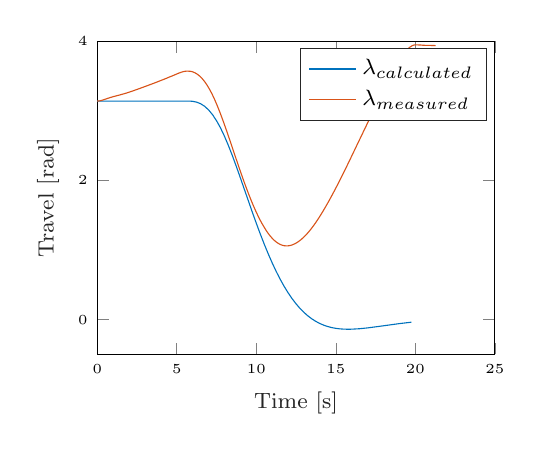
\begin{tikzpicture}

\begin{axis}[%
width=5.05cm,
height=3.975cm,
at={(0cm,0cm)},
scale only axis,
xmin=0,
xmax=25,
xlabel style={font=\color{white!15!black}},
xlabel={\footnotesize{Time [s]}},
ymin=-0.5,
ymax=4,
ylabel style={font=\color{white!15!black}},
ylabel={\footnotesize{Travel [rad]}},
ticklabel style = {font = \tiny},
axis background/.style={fill=white},
legend style={legend cell align=left, align=left, draw=white!15!black, font = \footnotesize}
]
\addplot [color=mycolor1]
  table[row sep=crcr]{%
0	3.14159265358979\\
5.75	3.14159265358979\\
6	3.13784214136253\\
6.25	3.12621555345805\\
6.5	3.10330930003011\\
6.75	3.06662741519147\\
7	3.01445392239469\\
7.25	2.94565627711845\\
7.5	2.85950776329499\\
7.75	2.75580734250692\\
8	2.63554349001547\\
8.25	2.50073168557186\\
8.5	2.35404209831692\\
8.75	2.1984468746386\\
9	2.03695272015638\\
9.75	1.54437252933372\\
10	1.38511969371918\\
10.25	1.23133807241257\\
10.5	1.08434498866704\\
10.75	0.945162915392995\\
11	0.814546237124432\\
11.25	0.693009826057356\\
11.5	0.580857859297378\\
11.75	0.478211887509147\\
12	0.385037543804632\\
12.25	0.301169528213396\\
12.5	0.226334664945398\\
12.75	0.160172937370163\\
13	0.102256478457353\\
13.25	0.0521065444181019\\
13.5	0.00920853399330213\\
13.75	-0.0269748600105828\\
14	-0.0569922637217886\\
14.25	-0.0813938854829672\\
14.5	-0.100723308365883\\
14.75	-0.115510687412002\\
15	-0.126267226263266\\
15.25	-0.13348080913013\\
15.5	-0.137612667011616\\
15.75	-0.139094961381911\\
16	-0.138329173892583\\
16.5	-0.131501025116556\\
17	-0.119706236352794\\
17.75	-0.0971329100931975\\
19	-0.0579432931566188\\
19.75	-0.0378837698859726\\
};
\addlegendentry{$\lambda{}_{\text{calculated}}$}

\addplot [color=mycolor2]
  table[row sep=crcr]{%
0	3.14159265358979\\
0.111999999999998	3.14312663437768\\
0.117999999999999	3.14389362477162\\
0.178000000000001	3.14542760555951\\
0.184000000000001	3.14619459595345\\
0.218	3.14772857674134\\
0.224	3.14849556713528\\
0.268000000000001	3.15002954792316\\
0.274000000000001	3.15079653831711\\
0.297999999999998	3.15233051910499\\
0.303999999999998	3.15309750949893\\
0.329999999999998	3.15463149028682\\
0.335999999999999	3.15539848068076\\
0.359999999999999	3.15693246146865\\
0.366	3.15769945186259\\
0.398	3.15923343265048\\
0.405999999999999	3.16076741343836\\
0.431999999999999	3.16230139422625\\
0.437999999999999	3.16306838462019\\
0.462	3.16460236540808\\
0.468	3.16536935580202\\
0.488	3.16690333658991\\
0.494	3.16767032698385\\
0.52	3.16920430777174\\
0.526	3.16997129816568\\
0.550000000000001	3.17150527895356\\
0.556000000000001	3.17227226934751\\
0.577999999999999	3.17380625013539\\
0.584	3.17457324052933\\
0.608000000000001	3.17610722131722\\
0.614000000000001	3.17687421171116\\
0.634	3.17840819249905\\
0.640000000000001	3.17917518289299\\
0.664000000000001	3.18070916368088\\
0.670000000000002	3.18147615407482\\
0.693999999999999	3.18301013486271\\
0.699999999999999	3.18377712525665\\
0.728000000000002	3.18531110604453\\
0.734000000000002	3.18607809643848\\
0.756	3.18761207722636\\
0.762	3.18837906762031\\
0.788	3.18991304840819\\
0.794	3.19068003880214\\
0.818000000000001	3.19221401959002\\
0.824000000000002	3.19298100998396\\
0.853999999999999	3.19451499077185\\
0.859999999999999	3.19528198116579\\
0.888000000000002	3.19681596195367\\
0.893999999999998	3.19758295234762\\
0.922000000000001	3.1991169331355\\
0.928000000000001	3.19988392352945\\
0.957999999999998	3.20141790431733\\
0.963999999999999	3.20218489471128\\
0.992000000000001	3.20371887549916\\
0.998000000000001	3.2044858658931\\
1.028	3.20601984668099\\
1.034	3.20678683707493\\
1.066	3.20832081786282\\
1.072	3.20908780825676\\
1.104	3.21062178904465\\
1.11	3.21138877943859\\
1.144	3.21292276022648\\
1.15	3.21368975062042\\
1.18	3.2152237314083\\
1.186	3.21599072180225\\
1.22	3.21752470259013\\
1.226	3.21829169298407\\
1.258	3.21982567377196\\
1.264	3.2205926641659\\
1.298	3.22212664495379\\
1.304	3.22289363534773\\
1.336	3.22442761613562\\
1.342	3.22519460652956\\
1.376	3.22672858731745\\
1.382	3.22749557771139\\
1.412	3.22902955849927\\
1.418	3.22979654889322\\
1.452	3.2313305296811\\
1.458	3.23209752007505\\
1.488	3.23363150086293\\
1.494	3.23439849125688\\
1.526	3.23593247204476\\
1.532	3.2366994624387\\
1.56	3.23823344322659\\
1.566	3.23900043362053\\
1.598	3.24053441440842\\
1.604	3.24130140480236\\
1.634	3.24283538559025\\
1.64	3.24360237598419\\
1.67	3.24513635677208\\
1.676	3.24590334716602\\
1.7	3.2474373279539\\
1.706	3.24820431834785\\
1.736	3.24973829913573\\
1.742	3.25050528952967\\
1.77	3.25203927031756\\
1.776	3.2528062607115\\
1.804	3.25434024149939\\
1.81	3.25510723189333\\
1.836	3.25664121268122\\
1.842	3.25740820307516\\
1.868	3.25894218386305\\
1.874	3.25970917425699\\
1.9	3.26124315504487\\
1.906	3.26201014543881\\
1.93	3.2635441262267\\
1.936	3.26431111662064\\
1.962	3.26584509740853\\
1.968	3.26661208780247\\
1.992	3.26814606859036\\
1.998	3.2689130589843\\
2.024	3.27044703977219\\
2.03	3.27121403016613\\
2.054	3.27274801095401\\
2.06	3.27351500134796\\
2.082	3.27504898213584\\
2.088	3.27581597252979\\
2.114	3.27734995331767\\
2.12	3.27811694371162\\
2.142	3.2796509244995\\
2.148	3.28041791489344\\
2.172	3.28195189568133\\
2.178	3.28271888607527\\
2.2	3.28425286686316\\
2.206	3.2850198572571\\
2.23	3.28655383804499\\
2.236	3.28732082843893\\
2.26	3.28885480922682\\
2.266	3.28962179962076\\
2.288	3.29115578040864\\
2.294	3.29192277080259\\
2.316	3.29345675159047\\
2.322	3.29422374198441\\
2.344	3.2957577227723\\
2.35	3.29652471316624\\
2.372	3.29805869395413\\
2.378	3.29882568434807\\
2.4	3.30035966513596\\
2.406	3.3011266555299\\
2.428	3.30266063631779\\
2.434	3.30342762671173\\
2.458	3.30496160749961\\
2.464	3.30572859789356\\
2.486	3.30726257868144\\
2.492	3.30802956907539\\
2.512	3.30956354986327\\
2.518	3.31033054025722\\
2.54	3.3118645210451\\
2.546	3.31263151143904\\
2.568	3.31416549222693\\
2.574	3.31493248262087\\
2.596	3.31646646340876\\
2.602	3.3172334538027\\
2.624	3.31876743459058\\
2.63	3.31953442498453\\
2.652	3.32106840577242\\
2.658	3.32183539616636\\
2.68	3.32336937695424\\
2.686	3.32413636734818\\
2.706	3.32567034813607\\
2.712	3.32643733853001\\
2.734	3.3279713193179\\
2.74	3.32873830971184\\
2.762	3.33027229049973\\
2.768	3.33103928089367\\
2.79	3.33257326168156\\
2.796	3.3333402520755\\
2.818	3.33487423286338\\
2.824	3.33564122325733\\
2.846	3.33717520404521\\
2.852	3.33794219443915\\
2.874	3.33947617522704\\
2.88	3.34024316562098\\
2.902	3.34177714640887\\
2.908	3.34254413680281\\
2.928	3.3440781175907\\
2.934	3.34484510798464\\
2.956	3.34637908877253\\
2.962	3.34714607916647\\
2.984	3.34868005995435\\
2.99	3.3494470503483\\
3.012	3.35098103113618\\
3.018	3.35174802153013\\
3.038	3.35328200231801\\
3.044	3.35404899271196\\
3.066	3.35558297349984\\
3.072	3.35634996389378\\
3.094	3.35788394468167\\
3.1	3.35865093507561\\
3.12	3.3601849158635\\
3.126	3.36095190625744\\
3.148	3.36248588704533\\
3.154	3.36325287743927\\
3.176	3.36478685822716\\
3.182	3.3655538486211\\
3.202	3.36708782940898\\
3.208	3.36785481980293\\
3.228	3.36938880059081\\
3.234	3.37015579098475\\
3.256	3.37168977177264\\
3.262	3.37245676216658\\
3.284	3.37399074295447\\
3.292	3.37552472374236\\
3.318	3.37705870453024\\
3.324	3.37782569492418\\
3.344	3.37935967571207\\
3.35	3.38012666610601\\
3.372	3.3816606468939\\
3.378	3.38242763728784\\
3.398	3.38396161807572\\
3.404	3.38472860846967\\
3.424	3.38626258925755\\
3.43	3.3870295796515\\
3.45	3.38856356043938\\
3.456	3.38933055083332\\
3.478	3.39086453162121\\
3.484	3.39163152201515\\
3.504	3.39316550280304\\
3.51	3.39393249319698\\
3.53	3.39546647398487\\
3.536	3.39623346437881\\
3.556	3.3977674451667\\
3.562	3.39853443556064\\
3.584	3.40006841634852\\
3.59	3.40083540674247\\
3.61	3.40236938753035\\
3.616	3.40313637792429\\
3.636	3.40467035871218\\
3.642	3.40543734910612\\
3.66	3.40697132989401\\
3.666	3.40773832028795\\
3.688	3.40927230107584\\
3.694	3.41003929146978\\
3.714	3.41157327225767\\
3.72	3.41234026265161\\
3.74	3.41387424343949\\
3.746	3.41464123383344\\
3.766	3.41617521462132\\
3.772	3.41694220501527\\
3.792	3.41847618580315\\
3.798	3.4192431761971\\
3.818	3.42077715698498\\
3.824	3.42154414737892\\
3.844	3.42307812816681\\
3.85	3.42384511856075\\
3.87	3.42537909934864\\
3.876	3.42614608974258\\
3.896	3.42768007053046\\
3.902	3.42844706092441\\
3.922	3.4299810417123\\
3.928	3.43074803210624\\
3.948	3.43228201289412\\
3.954	3.43304900328807\\
3.972	3.43458298407595\\
3.978	3.43534997446989\\
3.998	3.43688395525778\\
4.004	3.43765094565172\\
4.024	3.43918492643961\\
4.03	3.43995191683355\\
4.05	3.44148589762144\\
4.056	3.44225288801538\\
4.076	3.44378686880327\\
4.082	3.44455385919721\\
4.1	3.44608783998509\\
4.106	3.44685483037903\\
4.126	3.44838881116692\\
4.132	3.44915580156086\\
4.152	3.45068978234875\\
4.158	3.45145677274269\\
4.178	3.45299075353058\\
4.184	3.45375774392452\\
4.202	3.45529172471241\\
4.208	3.45605871510635\\
4.228	3.45759269589423\\
4.234	3.45835968628818\\
4.254	3.45989366707606\\
4.262	3.46142764786395\\
4.286	3.46296162865184\\
4.292	3.46372861904578\\
4.312	3.46526259983366\\
4.318	3.46602959022761\\
4.336	3.46756357101549\\
4.342	3.46833056140943\\
4.36	3.46986454219732\\
4.366	3.47063153259126\\
4.386	3.47216551337915\\
4.392	3.47293250377309\\
4.41	3.47446648456098\\
4.416	3.47523347495492\\
4.434	3.47676745574281\\
4.44	3.47753444613675\\
4.46	3.47906842692463\\
4.466	3.47983541731858\\
4.484	3.48136939810646\\
4.49	3.4821363885004\\
4.508	3.48367036928829\\
4.514	3.48443735968224\\
4.534	3.48597134047012\\
4.542	3.48750532125801\\
4.566	3.48903930204589\\
4.572	3.48980629243983\\
4.59	3.49134027322772\\
4.596	3.49210726362166\\
4.616	3.49364124440955\\
4.624	3.49517522519743\\
4.648	3.49670920598532\\
4.656	3.49824318677321\\
4.68	3.49977716756109\\
4.686	3.50054415795503\\
4.704	3.50207813874292\\
4.71	3.50284512913686\\
4.728	3.50437910992475\\
4.734	3.50514610031869\\
4.752	3.50668008110658\\
4.758	3.50744707150052\\
4.778	3.50898105228841\\
4.786	3.51051503307629\\
4.808	3.51204901386417\\
4.814	3.51281600425812\\
4.832	3.514349985046\\
4.838	3.51511697543995\\
4.856	3.51665095622783\\
4.862	3.51741794662178\\
4.88	3.51895192740966\\
4.886	3.5197189178036\\
4.904	3.52125289859149\\
4.91	3.52201988898543\\
4.928	3.52355386977332\\
4.934	3.52432086016726\\
4.954	3.52585484095515\\
4.962	3.52738882174303\\
4.984	3.52892280253092\\
4.992	3.5304567833188\\
5.016	3.53199076410669\\
5.024	3.53352474489457\\
5.048	3.53505872568246\\
5.054	3.5358257160764\\
5.072	3.53735969686429\\
5.078	3.53812668725823\\
5.098	3.53966066804612\\
5.106	3.541194648834\\
5.13	3.54272862962189\\
5.136	3.54349562001583\\
5.154	3.54502960080372\\
5.16	3.54579659119766\\
5.18	3.54733057198554\\
5.186	3.54809756237949\\
5.208	3.54963154316737\\
5.214	3.55039853356132\\
5.236	3.5519325143492\\
5.244	3.55346649513709\\
5.272	3.55500047592497\\
5.278	3.55576746631892\\
5.304	3.5573014471068\\
5.31	3.55806843750074\\
5.336	3.55960241828863\\
5.342	3.56036940868257\\
5.372	3.56190338947046\\
5.378	3.5626703798644\\
5.414	3.56420436065229\\
5.42	3.56497135104623\\
5.458	3.56650533183412\\
5.464	3.56727232222806\\
5.514	3.56880630301594\\
5.52	3.56957329340989\\
5.6	3.57110727419777\\
5.606	3.57187426459172\\
5.834	3.57034028380383\\
5.84	3.56957329340989\\
5.89	3.568039312622\\
5.896	3.56727232222806\\
5.934	3.56573834144017\\
5.94	3.56497135104623\\
5.972	3.56343737025835\\
5.978	3.5626703798644\\
6.002	3.56113639907652\\
6.008	3.56036940868257\\
6.03	3.55883542789469\\
6.036	3.55806843750074\\
6.058	3.55653445671286\\
6.064	3.55576746631892\\
6.082	3.55423348553103\\
6.09	3.55269950474315\\
6.112	3.55116552395526\\
6.12	3.54963154316737\\
6.14	3.54809756237949\\
6.148	3.5465635815916\\
6.166	3.54502960080372\\
6.174	3.54349562001583\\
6.188	3.54196163922795\\
6.194	3.541194648834\\
6.208	3.53966066804612\\
6.216	3.53812668725823\\
6.23	3.53659270647035\\
6.238	3.53505872568246\\
6.25	3.53352474489457\\
6.258	3.53199076410669\\
6.272	3.5304567833188\\
6.28	3.52892280253092\\
6.29	3.52738882174303\\
6.298	3.52585484095515\\
6.31	3.52432086016726\\
6.32	3.52201988898543\\
6.332	3.52048590819755\\
6.34	3.51895192740966\\
6.35	3.51741794662178\\
6.36	3.51511697543995\\
6.372	3.51358299465206\\
6.382	3.51128202347023\\
6.392	3.50974804268235\\
6.402	3.50744707150052\\
6.412	3.50591309071263\\
6.422	3.5036121195308\\
6.432	3.50207813874292\\
6.442	3.49977716756109\\
6.45	3.49824318677321\\
6.462	3.49517522519743\\
6.472	3.49364124440955\\
6.484	3.49057328283378\\
6.494	3.48903930204589\\
6.508	3.48520435007618\\
6.518	3.48367036928829\\
6.532	3.47983541731858\\
6.54	3.47830143653069\\
6.552	3.47523347495492\\
6.56	3.47369949416704\\
6.574	3.46986454219732\\
6.582	3.46833056140943\\
6.596	3.46449560943972\\
6.604	3.46296162865184\\
6.622	3.45759269589423\\
6.63	3.45605871510635\\
6.646	3.45145677274269\\
6.652	3.44992279195481\\
6.668	3.44532084959115\\
6.676	3.44378686880327\\
6.698	3.43688395525778\\
6.704	3.43534997446989\\
6.722	3.4299810417123\\
6.728	3.42844706092441\\
6.75	3.42154414737892\\
6.756	3.42001016659104\\
6.78	3.41234026265161\\
6.786	3.41080628186372\\
6.816	3.40083540674247\\
6.822	3.39930142595458\\
6.864	3.38472860846967\\
6.87	3.38319462768178\\
6.954	3.35251501192407\\
6.958	3.35098103113618\\
7.098	3.2957577227723\\
7.104	3.29268976119653\\
7.146	3.27504898213584\\
7.152	3.27198102056007\\
7.184	3.2581751934691\\
7.19	3.25510723189333\\
7.216	3.24360237598419\\
7.222	3.24053441440842\\
7.244	3.23056353928716\\
7.25	3.22749557771139\\
7.27	3.21829169298407\\
7.276	3.2152237314083\\
7.294	3.20678683707493\\
7.302	3.20218489471128\\
7.324	3.19221401959002\\
7.332	3.18761207722636\\
7.35	3.17917518289299\\
7.358	3.17457324052933\\
7.374	3.16690333658991\\
7.38	3.16383537501413\\
7.394	3.15693246146865\\
7.402	3.15233051910499\\
7.416	3.14542760555951\\
7.424	3.14082566319585\\
7.438	3.13392274965037\\
7.446	3.12932080728671\\
7.458	3.12318488413517\\
7.466	3.11858294177151\\
7.48	3.11168002822602\\
7.49	3.10554410507448\\
7.502	3.09940818192294\\
7.51	3.09480623955928\\
7.522	3.08867031640774\\
7.532	3.0825343932562\\
7.544	3.07639847010465\\
7.552	3.071796527741\\
7.562	3.0664275949834\\
7.572	3.06029167183186\\
7.584	3.05415574868031\\
7.594	3.04801982552877\\
7.604	3.04265089277117\\
7.612	3.03804895040751\\
7.622	3.03268001764991\\
7.632	3.02654409449837\\
7.642	3.02117516174077\\
7.652	3.01503923858923\\
7.66	3.01043729622557\\
7.67	3.00430137307403\\
7.68	2.99893244031643\\
7.69	2.99279651716489\\
7.7	2.98742758440729\\
7.712	2.97975768046786\\
7.72	2.9751557381042\\
7.73	2.96901981495266\\
7.74	2.96365088219506\\
7.752	2.95598097825563\\
7.76	2.95137903589197\\
7.772	2.94370913195255\\
7.782	2.93834019919495\\
7.796	2.92913631446763\\
7.804	2.92453437210397\\
7.816	2.91686446816455\\
7.824	2.91226252580089\\
7.836	2.90459262186146\\
7.844	2.8999906794978\\
7.856	2.89232077555838\\
7.864	2.88771883319472\\
7.878	2.87851494846741\\
7.886	2.87391300610375\\
7.898	2.86624310216432\\
7.906	2.86164115980066\\
7.922	2.85090329428547\\
7.93	2.84630135192181\\
7.944	2.83709746719449\\
7.952	2.83249552483084\\
7.968	2.82175765931564\\
7.976	2.81715571695198\\
7.994	2.80488387064889\\
8.002	2.80028192828524\\
8.018	2.78954406277004\\
8.026	2.78494212040638\\
8.042	2.77420425489118\\
8.048	2.77036930292147\\
8.062	2.76116541819415\\
8.068	2.75733046622444\\
8.084	2.74659260070924\\
8.092	2.74199065834559\\
8.112	2.72818483125461\\
8.12	2.72358288889096\\
8.14	2.70977706179999\\
8.148	2.70517511943633\\
8.168	2.69136929234536\\
8.176	2.6867673499817\\
8.198	2.67142754210284\\
8.206	2.66682559973919\\
8.228	2.65148579186033\\
8.236	2.64688384949667\\
8.26	2.63001006082993\\
8.268	2.62540811846628\\
8.29	2.61006831058742\\
8.296	2.6062333586177\\
8.316	2.59242753152673\\
8.324	2.58782558916308\\
8.348	2.57095180049633\\
8.354	2.56711684852662\\
8.374	2.55331102143565\\
8.38	2.54947606946594\\
8.398	2.53720422316285\\
8.404	2.53336927119314\\
8.424	2.51956344410216\\
8.43	2.51572849213245\\
8.45	2.50192266504148\\
8.456	2.49808771307177\\
8.478	2.48274790519291\\
8.486	2.47814596282925\\
8.512	2.45973819337463\\
8.518	2.45590324140491\\
8.538	2.44209741431394\\
8.544	2.43826246234423\\
8.564	2.42445663525326\\
8.57	2.42062168328354\\
8.59	2.40681585619257\\
8.596	2.40298090422286\\
8.616	2.38917507713188\\
8.622	2.38534012516217\\
8.644	2.37000031728332\\
8.65	2.3661653653136\\
8.668	2.35389351901052\\
8.674	2.3500585670408\\
8.694	2.33625273994983\\
8.7	2.33241778798012\\
8.72	2.31861196088915\\
8.726	2.31477700891943\\
8.746	2.30097118182846\\
8.752	2.29713622985875\\
8.77	2.28486438355566\\
8.776	2.28102943158595\\
8.794	2.26875758528286\\
8.8	2.26492263331315\\
8.82	2.25111680622218\\
8.826	2.24728185425246\\
8.844	2.23501000794938\\
8.85	2.23117505597967\\
8.868	2.21890320967658\\
8.874	2.21506825770687\\
8.892	2.20279641140378\\
8.9	2.19819446904012\\
8.922	2.18285466116127\\
8.93	2.17825271879761\\
8.952	2.16291291091876\\
8.958	2.15907795894904\\
8.974	2.14834009343384\\
8.982	2.14373815107018\\
9.002	2.12993232397921\\
9.008	2.1260973720095\\
9.024	2.1153595064943\\
9.032	2.11075756413064\\
9.05	2.09848571782756\\
9.056	2.09465076585784\\
9.072	2.08391290034264\\
9.08	2.07931095797899\\
9.098	2.0670391116759\\
9.106	2.06243716931224\\
9.124	2.05016532300916\\
9.132	2.0455633806455\\
9.148	2.0348255151303\\
9.154	2.03099056316059\\
9.168	2.02178667843328\\
9.176	2.01718473606962\\
9.192	2.00644687055442\\
9.2	2.00184492819076\\
9.216	1.99110706267556\\
9.224	1.9865051203119\\
9.238	1.97730123558459\\
9.246	1.97269929322093\\
9.262	1.96196142770573\\
9.27	1.95735948534208\\
9.282	1.94968958140265\\
9.29	1.94508763903899\\
9.304	1.93588375431168\\
9.312	1.93128181194802\\
9.324	1.9236119080086\\
9.33	1.91977695603888\\
9.34	1.91364103288734\\
9.348	1.90903909052368\\
9.362	1.89983520579637\\
9.37	1.89523326343271\\
9.382	1.88756335949328\\
9.39	1.88296141712962\\
9.402	1.8752915131902\\
9.412	1.8699225804326\\
9.424	1.86225267649317\\
9.432	1.85765073412951\\
9.444	1.84998083019008\\
9.452	1.84537888782643\\
9.462	1.83924296467488\\
9.47	1.83464102231123\\
9.48	1.82850509915968\\
9.488	1.82390315679603\\
9.498	1.81776723364449\\
9.508	1.81239830088688\\
9.52	1.80472839694746\\
9.53	1.79935946418986\\
9.542	1.79168956025043\\
9.552	1.78632062749283\\
9.562	1.78018470434129\\
9.572	1.77481577158369\\
9.582	1.76867984843214\\
9.592	1.76331091567454\\
9.602	1.757174992523\\
9.612	1.7518060597654\\
9.622	1.74567013661386\\
9.632	1.74030120385626\\
9.642	1.73416528070472\\
9.652	1.72879634794712\\
9.66	1.72419440558346\\
9.67	1.71882547282586\\
9.68	1.71268954967432\\
9.692	1.70655362652278\\
9.702	1.70041770337123\\
9.714	1.69428178021969\\
9.724	1.68814585706815\\
9.736	1.68200993391661\\
9.744	1.67740799155295\\
9.756	1.67127206840141\\
9.766	1.66513614524986\\
9.78	1.65823323170438\\
9.79	1.65209730855284\\
9.804	1.64519439500735\\
9.812	1.64059245264369\\
9.824	1.63445652949215\\
9.832	1.6298545871285\\
9.844	1.62371866397695\\
9.852	1.6191167216133\\
9.866	1.61221380806781\\
9.874	1.60761186570415\\
9.888	1.60070895215867\\
9.896	1.59610700979501\\
9.912	1.58843710585558\\
9.92	1.58383516349193\\
9.936	1.5761652595525\\
9.944	1.57156331718884\\
9.96	1.56389341324941\\
9.966	1.56082545167364\\
9.98	1.55392253812816\\
9.986	1.55085457655238\\
10.002	1.54318467261296\\
10.01	1.5385827302493\\
10.03	1.52937884552198\\
10.038	1.52477690315833\\
10.06	1.51480602803707\\
10.066	1.5117380664613\\
10.086	1.50253418173399\\
10.094	1.49793223937033\\
10.118	1.48719437385513\\
10.124	1.48412641227936\\
10.148	1.47338854676416\\
10.154	1.47032058518839\\
10.178	1.45958271967319\\
10.184	1.45651475809742\\
10.212	1.44424291179433\\
10.218	1.44117495021856\\
10.25	1.42736912312759\\
10.256	1.42430116155182\\
10.296	1.40742737288507\\
10.302	1.4043594113093\\
10.364	1.37904872830919\\
10.37	1.37598076673342\\
10.632	1.2770390059148\\
10.638	1.27550502512691\\
10.68	1.260932207642\\
10.686	1.25939822685411\\
10.72	1.24789337094497\\
10.726	1.24635939015708\\
10.754	1.23715550542977\\
10.76	1.23562152464189\\
10.784	1.22795162070246\\
10.79	1.22641763991457\\
10.81	1.22028171676303\\
10.816	1.21874773597514\\
10.836	1.2126118128236\\
10.842	1.21107783203571\\
10.862	1.20494190888417\\
10.87	1.20340792809629\\
10.89	1.19727200494474\\
10.898	1.19573802415686\\
10.918	1.18960210100531\\
10.926	1.18806812021743\\
10.942	1.18346617785377\\
10.95	1.18193219706589\\
10.966	1.17733025470223\\
10.974	1.17579627391434\\
10.99	1.17119433155069\\
10.998	1.1696603507628\\
11.01	1.16659238918703\\
11.018	1.16505840839914\\
11.034	1.16045646603549\\
11.044	1.1589224852476\\
11.058	1.15508753327789\\
11.066	1.15355355249\\
11.078	1.15048559091423\\
11.088	1.14895161012635\\
11.1	1.14588364855057\\
11.108	1.14434966776269\\
11.118	1.14204869658086\\
11.126	1.14051471579297\\
11.136	1.13821374461115\\
11.144	1.13667976382326\\
11.154	1.13437879264143\\
11.164	1.13284481185354\\
11.174	1.13054384067172\\
11.184	1.12900985988383\\
11.194	1.12670888870201\\
11.204	1.12517490791412\\
11.214	1.12287393673229\\
11.224	1.1213399559444\\
11.234	1.11903898476258\\
11.246	1.11750500397469\\
11.256	1.11520403279286\\
11.268	1.11367005200498\\
11.278	1.11136908082315\\
11.29	1.10983510003526\\
11.298	1.10830111924738\\
11.31	1.10676713845949\\
11.32	1.10446616727766\\
11.334	1.10293218648978\\
11.342	1.10139820570189\\
11.354	1.099864224914\\
11.362	1.09833024412612\\
11.376	1.09679626333823\\
11.384	1.09526228255035\\
11.398	1.09372830176246\\
11.406	1.09219432097458\\
11.42	1.09066034018669\\
11.428	1.0891263593988\\
11.444	1.08759237861092\\
11.452	1.08605839782303\\
11.47	1.08452441703515\\
11.478	1.08299043624726\\
11.498	1.08145645545938\\
11.506	1.07992247467149\\
11.526	1.0783884938836\\
11.532	1.07762150348966\\
11.55	1.07608752270178\\
11.556	1.07532053230783\\
11.576	1.07378655151995\\
11.582	1.07301956112601\\
11.602	1.07148558033812\\
11.608	1.07071858994418\\
11.634	1.06918460915629\\
11.64	1.06841761876235\\
11.668	1.06688363797446\\
11.674	1.06611664758052\\
11.71	1.06458266679264\\
11.716	1.06381567639869\\
11.758	1.06228169561081\\
11.764	1.06151470521687\\
11.856	1.05998072442898\\
11.862	1.05921373403504\\
12.032	1.06074771482292\\
12.038	1.06151470521687\\
12.09	1.06304868600475\\
12.096	1.06381567639869\\
12.136	1.06534965718658\\
12.142	1.06611664758052\\
12.176	1.0676506283684\\
12.182	1.06841761876235\\
12.21	1.06995159955024\\
12.216	1.07071858994418\\
12.24	1.07225257073206\\
12.246	1.07301956112601\\
12.27	1.07455354191389\\
12.276	1.07532053230783\\
12.296	1.07685451309572\\
12.302	1.07762150348966\\
12.322	1.07915548427755\\
12.328	1.07992247467149\\
12.346	1.08145645545938\\
12.354	1.08299043624726\\
12.376	1.08452441703515\\
12.384	1.08605839782303\\
12.404	1.08759237861092\\
12.412	1.0891263593988\\
12.43	1.09066034018669\\
12.436	1.09142733058063\\
12.45	1.09296131136852\\
12.458	1.09449529215641\\
12.476	1.09602927294429\\
12.484	1.09756325373218\\
12.498	1.09909723452006\\
12.506	1.10063121530795\\
12.522	1.10216519609583\\
12.53	1.10369917688372\\
12.544	1.10523315767161\\
12.552	1.10676713845949\\
12.566	1.10830111924738\\
12.574	1.10983510003526\\
12.586	1.11136908082315\\
12.594	1.11290306161103\\
12.608	1.11443704239892\\
12.616	1.11597102318681\\
12.628	1.11750500397469\\
12.636	1.11903898476258\\
12.648	1.12057296555046\\
12.658	1.12287393673229\\
12.67	1.12440791752018\\
12.678	1.12594189830806\\
12.69	1.12747587909595\\
12.7	1.12977685027777\\
12.712	1.13131083106566\\
12.72	1.13284481185354\\
12.73	1.13437879264143\\
12.74	1.13667976382326\\
12.752	1.13821374461115\\
12.762	1.14051471579297\\
12.772	1.14204869658086\\
12.78	1.14358267736874\\
12.79	1.14511665815663\\
12.8	1.14741762933846\\
12.81	1.14895161012635\\
12.82	1.15125258130817\\
12.83	1.15278656209606\\
12.84	1.15508753327789\\
12.85	1.15662151406577\\
12.86	1.1589224852476\\
12.868	1.16045646603549\\
12.878	1.16275743721732\\
12.888	1.1642914180052\\
12.898	1.16659238918703\\
12.906	1.16812636997492\\
12.916	1.17042734115675\\
12.924	1.17196132194463\\
12.934	1.17426229312646\\
12.944	1.17579627391434\\
12.956	1.17886423549011\\
12.964	1.180398216278\\
12.974	1.18269918745983\\
12.982	1.18423316824772\\
12.994	1.18730112982349\\
13.004	1.18883511061137\\
13.018	1.19267006258109\\
13.028	1.19420404336897\\
13.042	1.19803899533868\\
13.05	1.19957297612657\\
13.062	1.20264093770234\\
13.07	1.20417491849023\\
13.082	1.207242880066\\
13.09	1.20877686085388\\
13.104	1.2126118128236\\
13.112	1.21414579361149\\
13.124	1.21721375518726\\
13.132	1.21874773597514\\
13.146	1.22258268794486\\
13.154	1.22411666873274\\
13.17	1.2287186110964\\
13.178	1.23025259188428\\
13.194	1.23485453424794\\
13.202	1.23638851503583\\
13.216	1.24022346700554\\
13.222	1.24175744779343\\
13.236	1.24559239976314\\
13.244	1.24712638055103\\
13.26	1.25172832291468\\
13.266	1.25326230370257\\
13.28	1.25709725567228\\
13.288	1.25863123646017\\
13.308	1.26476715961171\\
13.316	1.2663011403996\\
13.336	1.27243706355114\\
13.344	1.27397104433902\\
13.364	1.28010696749057\\
13.37	1.28164094827845\\
13.386	1.28624289064211\\
13.392	1.28777687143\\
13.412	1.29391279458154\\
13.42	1.29544677536942\\
13.444	1.30311667930885\\
13.45	1.30465066009674\\
13.47	1.31078658324828\\
13.476	1.31232056403617\\
13.496	1.31845648718771\\
13.502	1.31999046797559\\
13.526	1.32766037191502\\
13.532	1.32919435270291\\
13.554	1.33609726624839\\
13.56	1.33763124703628\\
13.586	1.34606814136965\\
13.592	1.34760212215754\\
13.618	1.35603901649091\\
13.624	1.35757299727879\\
13.654	1.36754387240005\\
13.66	1.36907785318794\\
13.692	1.37981571870314\\
13.698	1.38134969949102\\
13.734	1.3936215457941\\
13.74	1.39515552658199\\
13.784	1.41049533446085\\
13.79	1.41202931524873\\
13.838	1.42890310391547\\
13.844	1.43043708470336\\
13.9	1.45037883494587\\
13.906	1.45191281573376\\
13.986	1.48105845070359\\
13.992	1.48259243149147\\
14.132	1.53474777827958\\
14.138	1.53628175906747\\
14.144	1.53934972064324\\
14.15	1.54088370143113\\
14.414	1.64366041421946\\
14.42	1.64672837579523\\
14.524	1.68814585706815\\
14.53	1.69121381864392\\
14.602	1.72035945361375\\
14.608	1.72342741518952\\
14.672	1.74950508858358\\
14.678	1.75257305015935\\
14.73	1.77404878118974\\
14.736	1.77711674276551\\
14.786	1.79782548340197\\
14.792	1.80089344497774\\
14.838	1.82006820482631\\
14.844	1.82313616640208\\
14.886	1.84077694546277\\
14.892	1.84384490703854\\
14.93	1.85995170531134\\
14.936	1.86301966688711\\
14.972	1.87835947476597\\
14.978	1.88142743634174\\
15.016	1.89753423461454\\
15.022	1.90060219619031\\
15.056	1.91517501367522\\
15.062	1.91824297525099\\
15.092	1.93128181194802\\
15.098	1.9343497735238\\
15.132	1.94892259100871\\
15.138	1.95199055258448\\
15.166	1.96426239888756\\
15.172	1.96733036046334\\
15.202	1.98036919716036\\
15.208	1.98343715873613\\
15.234	1.99494201464528\\
15.24	1.99800997622105\\
15.27	2.01104881291808\\
15.276	2.01411677449385\\
15.302	2.02562163040299\\
15.308	2.02868959197876\\
15.334	2.0401944478879\\
15.34	2.04326240946368\\
15.366	2.05476726537282\\
15.372	2.05783522694859\\
15.398	2.06934008285773\\
15.404	2.0724080444335\\
15.428	2.0831459099487\\
15.434	2.08621387152447\\
15.458	2.09695173703967\\
15.464	2.10001969861544\\
15.488	2.11075756413064\\
15.494	2.11382552570641\\
15.516	2.12379640082767\\
15.522	2.12686436240344\\
15.546	2.13760222791864\\
15.552	2.14067018949441\\
15.574	2.15064106461567\\
15.58	2.15370902619144\\
15.602	2.1636799013127\\
15.608	2.16674786288847\\
15.63	2.17671873800973\\
15.636	2.1797866995855\\
15.658	2.18975757470675\\
15.664	2.19282553628252\\
15.686	2.20279641140378\\
15.692	2.20586437297955\\
15.712	2.21506825770687\\
15.718	2.21813621928264\\
15.738	2.22734010400995\\
15.744	2.23040806558572\\
15.764	2.23961195031304\\
15.77	2.24267991188881\\
15.792	2.25265078701007\\
15.798	2.25571874858583\\
15.818	2.26492263331315\\
15.826	2.26952457567681\\
15.85	2.280262441192\\
15.856	2.28333040276778\\
15.876	2.29253428749509\\
15.882	2.29560224907086\\
15.902	2.30480613379818\\
15.908	2.30787409537395\\
15.928	2.31707798010126\\
15.934	2.32014594167703\\
15.952	2.3285828360104\\
15.958	2.33165079758617\\
15.978	2.34085468231349\\
15.984	2.34392264388926\\
16.004	2.35312652861657\\
16.012	2.35772847098023\\
16.036	2.36846633649543\\
16.042	2.3715342980712\\
16.06	2.37997119240457\\
16.066	2.38303915398035\\
16.086	2.39224303870766\\
16.092	2.39531100028343\\
16.11	2.4037478946168\\
16.116	2.40681585619257\\
16.134	2.41525275052594\\
16.14	2.41832071210171\\
16.16	2.42752459682903\\
16.168	2.43212653919268\\
16.192	2.44286440470788\\
16.198	2.44593236628366\\
16.216	2.45436926061702\\
16.222	2.4574372221928\\
16.24	2.46587411652617\\
16.246	2.46894207810194\\
16.264	2.47737897243531\\
16.27	2.48044693401108\\
16.29	2.4896508187384\\
16.298	2.49425276110205\\
16.32	2.50422363622331\\
16.326	2.50729159779908\\
16.346	2.51649548252639\\
16.352	2.51956344410216\\
16.37	2.52800033843554\\
16.376	2.53106830001131\\
16.394	2.53950519434468\\
16.4	2.54257315592045\\
16.42	2.55177704064776\\
16.426	2.55484500222354\\
16.444	2.56328189655691\\
16.45	2.56634985813268\\
16.468	2.57478675246605\\
16.474	2.57785471404182\\
16.494	2.58705859876913\\
16.5	2.59012656034491\\
16.52	2.59933044507222\\
16.528	2.60393238743588\\
16.552	2.61467025295108\\
16.558	2.61773821452685\\
16.578	2.62694209925416\\
16.586	2.63154404161782\\
16.61	2.64228190713302\\
16.616	2.64534986870879\\
16.636	2.6545537534361\\
16.644	2.65915569579976\\
16.668	2.66989356131496\\
16.674	2.67296152289073\\
16.694	2.68216540761804\\
16.7	2.68523336919381\\
16.72	2.69443725392113\\
16.728	2.69903919628479\\
16.752	2.70977706179999\\
16.758	2.71284502337576\\
16.778	2.72204890810307\\
16.784	2.72511686967884\\
16.804	2.73432075440616\\
16.812	2.73892269676981\\
16.836	2.74966056228501\\
16.842	2.75272852386078\\
16.862	2.7619324085881\\
16.868	2.76500037016387\\
16.888	2.77420425489118\\
16.894	2.77727221646695\\
16.914	2.78647610119427\\
16.92	2.78954406277004\\
16.94	2.79874794749735\\
16.946	2.80181590907312\\
16.966	2.81101979380044\\
16.972	2.81408775537621\\
16.992	2.82329164010352\\
16.998	2.82635960167929\\
17.018	2.83556348640661\\
17.024	2.83863144798238\\
17.046	2.84860232310363\\
17.052	2.85167028467941\\
17.072	2.86087416940672\\
17.078	2.86394213098249\\
17.1	2.87391300610375\\
17.106	2.87698096767952\\
17.126	2.88618485240683\\
17.132	2.8892528139826\\
17.152	2.89845669870992\\
17.158	2.90152466028569\\
17.18	2.91149553540695\\
17.186	2.91456349698272\\
17.208	2.92453437210397\\
17.214	2.92760233367975\\
17.236	2.937573208801\\
17.242	2.94064117037678\\
17.264	2.95061204549803\\
17.27	2.9536800070738\\
17.294	2.964417872589\\
17.3	2.96748583416477\\
17.322	2.97745670928603\\
17.328	2.9805246708618\\
17.352	2.991262536377\\
17.358	2.99433049795277\\
17.382	3.00506836346797\\
17.388	3.00813632504374\\
17.414	3.01964118095288\\
17.42	3.02270914252865\\
17.444	3.03344700804385\\
17.45	3.03651496961963\\
17.476	3.04801982552877\\
17.482	3.05108778710454\\
17.506	3.06182565261974\\
17.512	3.06489361419551\\
17.538	3.07639847010465\\
17.544	3.07946643168043\\
17.574	3.09250526837745\\
17.58	3.09557322995322\\
17.606	3.10707808586237\\
17.612	3.11014604743814\\
17.64	3.12241789374122\\
17.646	3.125485855317\\
17.676	3.13852469201402\\
17.682	3.14159265358979\\
17.71	3.15386449989288\\
17.716	3.15693246146865\\
17.746	3.16997129816568\\
17.752	3.17303925974145\\
17.784	3.18684508683242\\
17.79	3.18991304840819\\
17.822	3.20371887549916\\
17.828	3.20678683707493\\
17.862	3.22135965455985\\
17.868	3.22442761613562\\
17.902	3.23900043362053\\
17.908	3.2420683951963\\
17.946	3.2581751934691\\
17.952	3.26124315504487\\
17.99	3.27734995331767\\
17.996	3.28041791489344\\
18.034	3.29652471316624\\
18.04	3.29959267474202\\
18.082	3.3172334538027\\
18.088	3.32030141537847\\
18.132	3.3387091848331\\
18.138	3.34177714640887\\
18.184	3.36095190625744\\
18.19	3.36401986783321\\
18.24	3.38472860846967\\
18.246	3.38779657004544\\
18.3	3.41003929146978\\
18.306	3.41310725304555\\
18.362	3.43611696486384\\
18.368	3.43918492643961\\
18.432	3.46526259983366\\
18.438	3.46833056140943\\
18.504	3.49517522519743\\
18.51	3.49824318677321\\
18.59	3.5304567833188\\
18.596	3.53352474489457\\
18.688	3.57034028380383\\
18.694	3.5734082453796\\
18.806	3.61789368822829\\
18.81	3.61942766901617\\
18.906	3.65777718871331\\
18.912	3.66084515028908\\
18.916	3.66237913107697\\
19.108	3.73754418968337\\
19.114	3.74061215125914\\
19.118	3.74214613204702\\
19.41	3.85259274877479\\
19.416	3.85412672956267\\
19.46	3.86946653744153\\
19.466	3.87100051822942\\
19.488	3.8779034317749\\
19.494	3.87943741256279\\
19.51	3.88403935492644\\
19.516	3.88557333571433\\
19.53	3.88940828768405\\
19.538	3.89094226847193\\
19.552	3.89477722044164\\
19.56	3.89631120122953\\
19.572	3.8993791628053\\
19.58	3.90091314359319\\
19.592	3.90398110516896\\
19.602	3.90551508595684\\
19.614	3.90858304753261\\
19.624	3.9101170283205\\
19.632	3.91165100910839\\
19.642	3.91318498989627\\
19.652	3.9154859610781\\
19.664	3.91701994186598\\
19.672	3.91855392265387\\
19.682	3.92008790344176\\
19.69	3.92162188422964\\
19.702	3.92315586501753\\
19.71	3.92468984580541\\
19.722	3.9262238265933\\
19.73	3.92775780738118\\
19.744	3.92929178816907\\
19.752	3.93082576895696\\
19.766	3.93235974974484\\
19.774	3.93389373053273\\
19.792	3.93542771132061\\
19.8	3.9369616921085\\
19.82	3.93849567289638\\
19.828	3.94002965368427\\
19.85	3.94156363447216\\
19.856	3.9423306248661\\
19.876	3.94386460565399\\
19.882	3.94463159604793\\
19.912	3.94616557683581\\
19.918	3.94693256722976\\
19.96	3.94846654801764\\
19.966	3.94923353841158\\
20.344	3.9476995576237\\
20.35	3.94693256722976\\
20.452	3.94539858644187\\
20.458	3.94463159604793\\
20.588	3.94309761526004\\
20.594	3.9423306248661\\
21.106	3.94079664407821\\
21.112	3.94002965368427\\
21.28	3.93926266329033\\
};
\addlegendentry{$\lambda{}_{\text{measured}}$}

\end{axis}
\end{tikzpicture}%

        %\caption{Calculated and measured travel with weight q=1}
        \label{fig:2_travel_q10}
    \end{subfigure}%
    ~
    \begin{subfigure}[t]{0.5\textwidth}
        % This file was created by matlab2tikz.
%
%The latest updates can be retrieved from
%  http://www.mathworks.com/matlabcentral/fileexchange/22022-matlab2tikz-matlab2tikz
%where you can also make suggestions and rate matlab2tikz.
%
\definecolor{mycolor1}{rgb}{0.00000,0.44700,0.74100}%
\definecolor{mycolor2}{rgb}{0.85000,0.32500,0.09800}%
\definecolor{mycolor3}{rgb}{0.92900,0.69400,0.12500}%
%
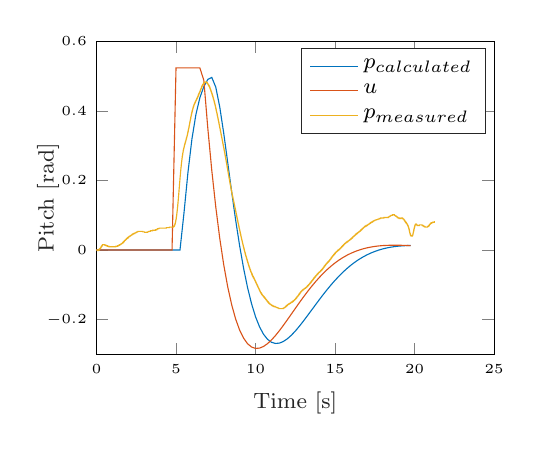
\begin{tikzpicture}

\begin{axis}[%
width=5.05cm,
height=3.975cm,
at={(0cm,0cm)},
scale only axis,
xmin=0,
xmax=25,
xlabel style={font=\color{white!15!black}},
xlabel={\footnotesize{Time [s]}},
ymin=-0.3,
ymax=0.6,
ylabel style={font=\color{white!15!black}},
ylabel={\footnotesize{Pitch [rad]}},
ylabel shift = -0.4cm,
ticklabel style = {font = \tiny},
axis background/.style={fill=white},
legend style={legend cell align=left, align=left, draw=white!15!black, font = \footnotesize}
]
\addplot [color=mycolor1]
  table[row sep=crcr]{%
0	0\\
5.25	0\\
5.5	0.106028752058414\\
5.75	0.222660379322271\\
6	0.31888147181499\\
6.25	0.38944360630968\\
6.5	0.437955073774344\\
6.75	0.469972642300633\\
7	0.490517248769844\\
7.25	0.496200699780641\\
7.5	0.46825603728232\\
7.75	0.411277472789379\\
8	0.335790530038274\\
8.25	0.251766547885314\\
8.5	0.166765559933022\\
8.75	0.0858590575835834\\
9	0.0121102638823594\\
9.25	-0.0528711229804344\\
9.5	-0.108461341465627\\
9.75	-0.154673812578718\\
10	-0.191915163126851\\
10.25	-0.220820955225122\\
10.5	-0.242147762302437\\
10.75	-0.256703442461301\\
11	-0.265302672902088\\
11.25	-0.268738967600775\\
11.5	-0.267767399444516\\
11.75	-0.263094291207882\\
12	-0.255371482600594\\
12.25	-0.245193642418521\\
12.5	-0.233097639386244\\
12.75	-0.219563326360962\\
13	-0.205015305715971\\
13.5	-0.174315457815457\\
14	-0.143393457924375\\
14.25	-0.128405724505996\\
14.5	-0.113953756103406\\
14.75	-0.100161039042391\\
15	-0.0871218208575542\\
15.25	-0.0749044118691806\\
15.5	-0.0635543359566455\\
15.75	-0.0530973085168611\\
16	-0.043542025827854\\
16.25	-0.0348827554096367\\
16.5	-0.0271017215857974\\
16.75	-0.020171284377728\\
17	-0.0140559131741682\\
17.25	-0.00871395937011599\\
17.5	-0.00409923441524285\\
17.75	-0.000162401503033038\\
18	0.00314780948346538\\
18.25	0.00588355312970634\\
18.5	0.00809697440598711\\
18.75	0.00983945756707527\\
19	0.0111610060698091\\
19.5	0.0127315101292069\\
19.75	0.0130695844848603\\
};
\addlegendentry{$p_{\text{calculated}}$}

\addplot [color=mycolor2]
  table[row sep=crcr]{%
0	0\\
4.75	0\\
5	0.523598775597101\\
6.5	0.523598775584638\\
6.75	0.487893582369146\\
7	0.349712272970329\\
7.25	0.22862490598752\\
7.5	0.123618574063489\\
7.75	0.0336217301827233\\
8	-0.0424741106382491\\
8.25	-0.105795938802146\\
8.5	-0.157472185579472\\
8.75	-0.198617522627131\\
9	-0.230319759815991\\
9.25	-0.253628897126461\\
9.5	-0.269548272017836\\
9.75	-0.279027674521721\\
10	-0.282958263707055\\
10.25	-0.282169100662802\\
10.5	-0.277425107610593\\
10.75	-0.269426265447027\\
11	-0.258807869810095\\
11.25	-0.246141676632835\\
11.5	-0.231937780759946\\
11.75	-0.216647084682727\\
12	-0.200664228210133\\
12.75	-0.151735543295892\\
13	-0.135924308423043\\
13.25	-0.120671512210237\\
13.5	-0.106108617293962\\
13.75	-0.0923361246412391\\
14	-0.0794270625626474\\
14.25	-0.0674303160084335\\
14.5	-0.0563737734923606\\
14.75	-0.0462672752404636\\
15	-0.037105351654116\\
15.25	-0.0288697459504981\\
15.5	-0.0215317189441642\\
15.75	-0.0150541374091304\\
16	-0.00939335036109767\\
16.25	-0.00450085997416139\\
16.5	-0.000324795745033413\\
16.75	0.00318879801088912\\
17	0.00609485015653632\\
17.25	0.00844831429271764\\
17.5	0.0103033714873497\\
17.75	0.0117127715715064\\
18	0.01272730040521\\
18.5	0.0137626543399492\\
19	0.0137629568098987\\
19.5	0.0130330358357753\\
19.75	0.0124756730078737\\
};
\addlegendentry{$u$}

\addplot [color=mycolor3]
  table[row sep=crcr]{%
0	0\\
0.0539999999999985	0\\
0.0560000000000009	-0.00153398078788669\\
0.111999999999998	-0.00153398078788669\\
0.114000000000001	0\\
0.172000000000001	0\\
0.173999999999999	0.00153398078788669\\
0.187999999999999	0.00153398078788669\\
0.190000000000001	0.00306796157576983\\
0.216000000000001	0.00306796157576983\\
0.218	0.00460194236365652\\
0.254000000000001	0.00460194236365652\\
0.256	0.00613592315154321\\
0.274000000000001	0.00613592315154321\\
0.276	0.0076699039394299\\
0.288	0.0076699039394299\\
0.289999999999999	0.00920388472731304\\
0.309999999999999	0.00920388472731304\\
0.312000000000001	0.0107378655151997\\
0.332000000000001	0.0107378655151997\\
0.334	0.0122718463030864\\
0.359999999999999	0.0122718463030864\\
0.361999999999998	0.0138058270909696\\
0.390000000000001	0.0138058270909696\\
0.391999999999999	0.0153398078788562\\
0.524000000000001	0.0153398078788562\\
0.526	0.0138058270909696\\
0.603999999999999	0.0138058270909696\\
0.606000000000002	0.0122718463030864\\
0.678000000000001	0.0122718463030864\\
0.68	0.0107378655151997\\
0.783999999999999	0.0107378655151997\\
0.786000000000001	0.00920388472731304\\
1.212	0.00920388472731304\\
1.214	0.0107378655151997\\
1.322	0.0107378655151997\\
1.324	0.0122718463030864\\
1.396	0.0122718463030864\\
1.398	0.0138058270909696\\
1.46	0.0138058270909696\\
1.462	0.0153398078788562\\
1.516	0.0153398078788562\\
1.518	0.0168737886667429\\
1.568	0.0168737886667429\\
1.57	0.0184077694546261\\
1.61	0.0184077694546261\\
1.612	0.0199417502425128\\
1.65	0.0199417502425128\\
1.652	0.0214757310303995\\
1.69	0.0214757310303995\\
1.692	0.0230097118182861\\
1.712	0.0230097118182861\\
1.714	0.0245436926061693\\
1.748	0.0245436926061693\\
1.75	0.026077673394056\\
1.772	0.026077673394056\\
1.774	0.0276116541819427\\
1.81	0.0276116541819427\\
1.812	0.0291456349698258\\
1.848	0.0291456349698258\\
1.85	0.0306796157577125\\
1.874	0.0306796157577125\\
1.876	0.0322135965455992\\
1.91	0.0322135965455992\\
1.912	0.0337475773334859\\
1.952	0.0337475773334859\\
1.954	0.035281558121369\\
1.996	0.035281558121369\\
1.998	0.0368155389092557\\
2.032	0.0368155389092557\\
2.034	0.0383495196971424\\
2.074	0.0383495196971424\\
2.076	0.0398835004850255\\
2.13	0.0398835004850255\\
2.132	0.0414174812729122\\
2.172	0.0414174812729122\\
2.174	0.0429514620607989\\
2.226	0.0429514620607989\\
2.228	0.0444854428486821\\
2.272	0.0444854428486821\\
2.274	0.0460194236365687\\
2.334	0.0460194236365687\\
2.336	0.0475534044244554\\
2.41	0.0475534044244554\\
2.412	0.0490873852123421\\
2.482	0.0490873852123421\\
2.484	0.0506213660002253\\
2.532	0.0506213660002253\\
2.534	0.052155346788112\\
2.604	0.052155346788112\\
2.606	0.0536893275759986\\
2.918	0.0536893275759986\\
2.92	0.052155346788112\\
3.022	0.052155346788112\\
3.024	0.0506213660002253\\
3.19	0.0506213660002253\\
3.192	0.052155346788112\\
3.276	0.052155346788112\\
3.278	0.0536893275759986\\
3.384	0.0536893275759986\\
3.386	0.0552233083638818\\
3.532	0.0552233083638818\\
3.534	0.0567572891517685\\
3.71	0.0567572891517685\\
3.712	0.0582912699396552\\
3.79	0.0582912699396552\\
3.792	0.0598252507275383\\
3.85	0.0598252507275383\\
3.852	0.061359231515425\\
3.938	0.061359231515425\\
3.94	0.0628932123033117\\
4.392	0.0628932123033117\\
4.394	0.0644271930911984\\
4.584	0.0644271930911984\\
4.586	0.0659611738790815\\
4.838	0.0659611738790815\\
4.84	0.0674951546669682\\
4.872	0.0674951546669682\\
4.874	0.0690291354548549\\
4.894	0.0690291354548549\\
4.896	0.070563116242738\\
4.91	0.070563116242738\\
4.912	0.0720970970306247\\
4.922	0.0720970970306247\\
4.924	0.0736310778185114\\
4.936	0.0736310778185114\\
4.938	0.0751650586063981\\
4.946	0.0751650586063981\\
4.948	0.0766990393942812\\
4.954	0.0766990393942812\\
4.956	0.0782330201821679\\
4.962	0.0782330201821679\\
4.964	0.0797670009700546\\
4.97	0.0797670009700546\\
4.972	0.0813009817579378\\
4.976	0.0813009817579378\\
4.978	0.0828349625458245\\
4.984	0.0828349625458245\\
4.986	0.0843689433337111\\
4.99	0.0843689433337111\\
4.992	0.0859029241215943\\
4.996	0.0859029241215943\\
4.998	0.087436904909481\\
5.002	0.087436904909481\\
5.004	0.0889708856973677\\
5.008	0.0889708856973677\\
5.01	0.0905048664852544\\
5.014	0.0905048664852544\\
5.016	0.0920388472731375\\
5.018	0.0920388472731375\\
5.02	0.0935728280610242\\
5.024	0.0935728280610242\\
5.026	0.0951068088489109\\
5.028	0.0951068088489109\\
5.03	0.096640789636794\\
5.032	0.096640789636794\\
5.034	0.0981747704246807\\
5.038	0.0981747704246807\\
5.04	0.0997087512125674\\
5.042	0.0997087512125674\\
5.044	0.101242732000454\\
5.046	0.101242732000454\\
5.048	0.102776712788337\\
5.05	0.102776712788337\\
5.052	0.104310693576224\\
5.054	0.104310693576224\\
5.056	0.105844674364111\\
5.058	0.105844674364111\\
5.06	0.107378655151994\\
5.062	0.107378655151994\\
5.064	0.10891263593988\\
5.066	0.10891263593988\\
5.068	0.110446616727767\\
5.07	0.110446616727767\\
5.072	0.11198059751565\\
5.074	0.11198059751565\\
5.076	0.113514578303537\\
5.078	0.113514578303537\\
5.082	0.11658253987931\\
5.084	0.11658253987931\\
5.086	0.118116520667193\\
5.088	0.118116520667193\\
5.092	0.121184482242967\\
5.094	0.121184482242967\\
5.096	0.12271846303085\\
5.098	0.12271846303085\\
5.102	0.125786424606623\\
5.104	0.125786424606623\\
5.106	0.127320405394507\\
5.108	0.127320405394507\\
5.112	0.13038836697028\\
5.114	0.13038836697028\\
5.118	0.13345632854605\\
5.12	0.13345632854605\\
5.122	0.134990309333936\\
5.124	0.134990309333936\\
5.128	0.138058270909706\\
5.13	0.138058270909706\\
5.136	0.142660213273366\\
5.138	0.142660213273366\\
5.14	0.144194194061249\\
5.142	0.144194194061249\\
5.148	0.148796136424906\\
5.15	0.148796136424906\\
5.154	0.151864098000679\\
5.156	0.151864098000679\\
5.162	0.156466040364336\\
5.164	0.156466040364336\\
5.168	0.159534001940106\\
5.17	0.159534001940106\\
5.176	0.164135944303762\\
5.178	0.164135944303762\\
5.182	0.167203905879536\\
5.184	0.167203905879536\\
5.19	0.171805848243192\\
5.192	0.171805848243192\\
5.198	0.176407790606849\\
5.2	0.176407790606849\\
5.204	0.179475752182618\\
5.206	0.179475752182618\\
5.212	0.184077694546279\\
5.214	0.184077694546279\\
5.22	0.188679636909935\\
5.222	0.188679636909935\\
5.228	0.193281579273592\\
5.23	0.193281579273592\\
5.234	0.196349540849361\\
5.236	0.196349540849361\\
5.24	0.199417502425135\\
5.242	0.199417502425135\\
5.248	0.204019444788791\\
5.25	0.204019444788791\\
5.254	0.207087406364561\\
5.256	0.207087406364561\\
5.262	0.211689348728218\\
5.264	0.211689348728218\\
5.266	0.213223329516104\\
5.268	0.213223329516104\\
5.274	0.217825271879761\\
5.276	0.217825271879761\\
5.28	0.220893233455531\\
5.282	0.220893233455531\\
5.284	0.222427214243417\\
5.286	0.222427214243417\\
5.29	0.225495175819191\\
5.292	0.225495175819191\\
5.296	0.228563137394961\\
5.298	0.228563137394961\\
5.3	0.230097118182847\\
5.302	0.230097118182847\\
5.306	0.233165079758617\\
5.308	0.233165079758617\\
5.312	0.23623304133439\\
5.314	0.23623304133439\\
5.316	0.237767022122274\\
5.318	0.237767022122274\\
5.32	0.23930100291016\\
5.322	0.23930100291016\\
5.326	0.24236896448593\\
5.328	0.24236896448593\\
5.33	0.243902945273817\\
5.332	0.243902945273817\\
5.334	0.245436926061704\\
5.336	0.245436926061704\\
5.34	0.248504887637473\\
5.342	0.248504887637473\\
5.344	0.25003886842536\\
5.346	0.25003886842536\\
5.348	0.251572849213247\\
5.35	0.251572849213247\\
5.352	0.25310683000113\\
5.354	0.25310683000113\\
5.356	0.254640810789017\\
5.358	0.254640810789017\\
5.36	0.256174791576903\\
5.362	0.256174791576903\\
5.364	0.257708772364786\\
5.366	0.257708772364786\\
5.368	0.259242753152673\\
5.37	0.259242753152673\\
5.372	0.26077673394056\\
5.374	0.26077673394056\\
5.376	0.262310714728443\\
5.38	0.262310714728443\\
5.382	0.26384469551633\\
5.384	0.26384469551633\\
5.386	0.265378676304216\\
5.388	0.265378676304216\\
5.39	0.266912657092103\\
5.392	0.266912657092103\\
5.394	0.268446637879986\\
5.398	0.268446637879986\\
5.4	0.269980618667873\\
5.402	0.269980618667873\\
5.404	0.27151459945576\\
5.408	0.27151459945576\\
5.41	0.273048580243643\\
5.412	0.273048580243643\\
5.414	0.274582561031529\\
5.418	0.274582561031529\\
5.42	0.276116541819416\\
5.424	0.276116541819416\\
5.426	0.277650522607303\\
5.43	0.277650522607303\\
5.432	0.279184503395186\\
5.434	0.279184503395186\\
5.436	0.280718484183073\\
5.442	0.280718484183073\\
5.444	0.282252464970959\\
5.446	0.282252464970959\\
5.448	0.283786445758842\\
5.452	0.283786445758842\\
5.454	0.285320426546729\\
5.46	0.285320426546729\\
5.462	0.286854407334616\\
5.466	0.286854407334616\\
5.468	0.288388388122499\\
5.474	0.288388388122499\\
5.476	0.289922368910386\\
5.48	0.289922368910386\\
5.482	0.291456349698272\\
5.488	0.291456349698272\\
5.49	0.292990330486159\\
5.496	0.292990330486159\\
5.498	0.294524311274042\\
5.504	0.294524311274042\\
5.506	0.296058292061929\\
5.512	0.296058292061929\\
5.514	0.297592272849815\\
5.522	0.297592272849815\\
5.524	0.299126253637699\\
5.53	0.299126253637699\\
5.532	0.300660234425585\\
5.538	0.300660234425585\\
5.54	0.302194215213472\\
5.546	0.302194215213472\\
5.548	0.303728196001359\\
5.556	0.303728196001359\\
5.558	0.305262176789242\\
5.566	0.305262176789242\\
5.568	0.306796157577129\\
5.574	0.306796157577129\\
5.576	0.308330138365015\\
5.584	0.308330138365015\\
5.586	0.309864119152898\\
5.594	0.309864119152898\\
5.596	0.311398099940785\\
5.604	0.311398099940785\\
5.606	0.312932080728672\\
5.614	0.312932080728672\\
5.616	0.314466061516555\\
5.622	0.314466061516555\\
5.624	0.316000042304442\\
5.632	0.316000042304442\\
5.634	0.317534023092328\\
5.64	0.317534023092328\\
5.642	0.319068003880215\\
5.65	0.319068003880215\\
5.652	0.320601984668098\\
5.658	0.320601984668098\\
5.66	0.322135965455985\\
5.668	0.322135965455985\\
5.67	0.323669946243871\\
5.676	0.323669946243871\\
5.678	0.325203927031755\\
5.684	0.325203927031755\\
5.686	0.326737907819641\\
5.692	0.326737907819641\\
5.694	0.328271888607528\\
5.7	0.328271888607528\\
5.702	0.329805869395411\\
5.708	0.329805869395411\\
5.71	0.331339850183298\\
5.716	0.331339850183298\\
5.718	0.332873830971185\\
5.724	0.332873830971185\\
5.726	0.334407811759071\\
5.732	0.334407811759071\\
5.734	0.335941792546954\\
5.738	0.335941792546954\\
5.74	0.337475773334841\\
5.746	0.337475773334841\\
5.748	0.339009754122728\\
5.752	0.339009754122728\\
5.754	0.340543734910611\\
5.76	0.340543734910611\\
5.762	0.342077715698498\\
5.768	0.342077715698498\\
5.77	0.343611696486384\\
5.776	0.343611696486384\\
5.778	0.345145677274271\\
5.78	0.345145677274271\\
5.782	0.346679658062154\\
5.788	0.346679658062154\\
5.79	0.348213638850041\\
5.796	0.348213638850041\\
5.798	0.349747619637927\\
5.802	0.349747619637927\\
5.804	0.351281600425811\\
5.808	0.351281600425811\\
5.81	0.352815581213697\\
5.816	0.352815581213697\\
5.818	0.354349562001584\\
5.822	0.354349562001584\\
5.824	0.355883542789467\\
5.828	0.355883542789467\\
5.83	0.357417523577354\\
5.834	0.357417523577354\\
5.836	0.35895150436524\\
5.84	0.35895150436524\\
5.842	0.360485485153127\\
5.848	0.360485485153127\\
5.85	0.36201946594101\\
5.854	0.36201946594101\\
5.856	0.363553446728897\\
5.86	0.363553446728897\\
5.862	0.365087427516784\\
5.866	0.365087427516784\\
5.868	0.366621408304667\\
5.872	0.366621408304667\\
5.874	0.368155389092554\\
5.88	0.368155389092554\\
5.882	0.36968936988044\\
5.886	0.36968936988044\\
5.888	0.371223350668327\\
5.892	0.371223350668327\\
5.894	0.37275733145621\\
5.898	0.37275733145621\\
5.9	0.374291312244097\\
5.906	0.374291312244097\\
5.908	0.375825293031983\\
5.912	0.375825293031983\\
5.914	0.377359273819867\\
5.92	0.377359273819867\\
5.922	0.378893254607753\\
5.926	0.378893254607753\\
5.928	0.38042723539564\\
5.932	0.38042723539564\\
5.934	0.381961216183523\\
5.938	0.381961216183523\\
5.94	0.38349519697141\\
5.946	0.38349519697141\\
5.948	0.385029177759296\\
5.952	0.385029177759296\\
5.954	0.386563158547183\\
5.958	0.386563158547183\\
5.96	0.388097139335066\\
5.966	0.388097139335066\\
5.968	0.389631120122953\\
5.974	0.389631120122953\\
5.976	0.39116510091084\\
5.98	0.39116510091084\\
5.982	0.392699081698723\\
5.988	0.392699081698723\\
5.99	0.394233062486609\\
5.996	0.394233062486609\\
5.998	0.395767043274496\\
6.004	0.395767043274496\\
6.006	0.397301024062379\\
6.012	0.397301024062379\\
6.014	0.398835004850266\\
6.02	0.398835004850266\\
6.022	0.400368985638153\\
6.026	0.400368985638153\\
6.028	0.401902966426039\\
6.038	0.401902966426039\\
6.04	0.403436947213923\\
6.046	0.403436947213923\\
6.048	0.404970928001809\\
6.054	0.404970928001809\\
6.056	0.406504908789696\\
6.064	0.406504908789696\\
6.066	0.408038889577579\\
6.074	0.408038889577579\\
6.076	0.409572870365466\\
6.084	0.409572870365466\\
6.086	0.411106851153352\\
6.096	0.411106851153352\\
6.098	0.412640831941239\\
6.106	0.412640831941239\\
6.108	0.414174812729122\\
6.116	0.414174812729122\\
6.118	0.415708793517009\\
6.128	0.415708793517009\\
6.13	0.417242774304896\\
6.14	0.417242774304896\\
6.142	0.418776755092779\\
6.152	0.418776755092779\\
6.154	0.420310735880665\\
6.168	0.420310735880665\\
6.17	0.421844716668552\\
6.182	0.421844716668552\\
6.184	0.423378697456435\\
6.196	0.423378697456435\\
6.198	0.424912678244322\\
6.212	0.424912678244322\\
6.214	0.426446659032209\\
6.226	0.426446659032209\\
6.228	0.427980639820095\\
6.242	0.427980639820095\\
6.244	0.429514620607979\\
6.258	0.429514620607979\\
6.26	0.431048601395865\\
6.274	0.431048601395865\\
6.276	0.432582582183752\\
6.292	0.432582582183752\\
6.294	0.434116562971635\\
6.308	0.434116562971635\\
6.31	0.435650543759522\\
6.324	0.435650543759522\\
6.326	0.437184524547408\\
6.338	0.437184524547408\\
6.34	0.438718505335295\\
6.354	0.438718505335295\\
6.356	0.440252486123178\\
6.368	0.440252486123178\\
6.37	0.441786466911065\\
6.384	0.441786466911065\\
6.386	0.443320447698952\\
6.398	0.443320447698952\\
6.4	0.444854428486835\\
6.412	0.444854428486835\\
6.414	0.446388409274721\\
6.428	0.446388409274721\\
6.43	0.447922390062608\\
6.442	0.447922390062608\\
6.444	0.449456370850491\\
6.454	0.449456370850491\\
6.456	0.450990351638378\\
6.47	0.450990351638378\\
6.472	0.452524332426265\\
6.484	0.452524332426265\\
6.486	0.454058313214151\\
6.498	0.454058313214151\\
6.5	0.455592294002034\\
6.51	0.455592294002034\\
6.512	0.457126274789921\\
6.524	0.457126274789921\\
6.526	0.458660255577808\\
6.538	0.458660255577808\\
6.54	0.460194236365691\\
6.55	0.460194236365691\\
6.552	0.461728217153578\\
6.562	0.461728217153578\\
6.564	0.463262197941464\\
6.576	0.463262197941464\\
6.578	0.464796178729351\\
6.588	0.464796178729351\\
6.59	0.466330159517234\\
6.602	0.466330159517234\\
6.604	0.467864140305121\\
6.616	0.467864140305121\\
6.618	0.469398121093008\\
6.63	0.469398121093008\\
6.632	0.470932101880891\\
6.646	0.470932101880891\\
6.648	0.472466082668777\\
6.662	0.472466082668777\\
6.664	0.474000063456664\\
6.678	0.474000063456664\\
6.68	0.475534044244547\\
6.698	0.475534044244547\\
6.7	0.477068025032434\\
6.716	0.477068025032434\\
6.718	0.478602005820321\\
6.74	0.478602005820321\\
6.742	0.480135986608207\\
6.766	0.480135986608207\\
6.768	0.48166996739609\\
6.816	0.48166996739609\\
6.818	0.483203948183977\\
6.902	0.483203948183977\\
6.904	0.48166996739609\\
6.946	0.48166996739609\\
6.948	0.480135986608207\\
6.976	0.480135986608207\\
6.978	0.478602005820321\\
7	0.478602005820321\\
7.002	0.477068025032434\\
7.022	0.477068025032434\\
7.024	0.475534044244547\\
7.04	0.475534044244547\\
7.042	0.474000063456664\\
7.058	0.474000063456664\\
7.06	0.472466082668777\\
7.076	0.472466082668777\\
7.078	0.470932101880891\\
7.092	0.470932101880891\\
7.094	0.469398121093008\\
7.108	0.469398121093008\\
7.11	0.467864140305121\\
7.122	0.467864140305121\\
7.124	0.466330159517234\\
7.136	0.466330159517234\\
7.138	0.464796178729351\\
7.148	0.464796178729351\\
7.15	0.463262197941464\\
7.162	0.463262197941464\\
7.164	0.461728217153578\\
7.174	0.461728217153578\\
7.176	0.460194236365691\\
7.186	0.460194236365691\\
7.188	0.458660255577808\\
7.198	0.458660255577808\\
7.2	0.457126274789921\\
7.212	0.457126274789921\\
7.214	0.455592294002034\\
7.222	0.455592294002034\\
7.224	0.454058313214151\\
7.232	0.454058313214151\\
7.234	0.452524332426265\\
7.244	0.452524332426265\\
7.246	0.450990351638378\\
7.256	0.450990351638378\\
7.258	0.449456370850491\\
7.266	0.449456370850491\\
7.268	0.447922390062608\\
7.276	0.447922390062608\\
7.278	0.446388409274721\\
7.286	0.446388409274721\\
7.288	0.444854428486835\\
7.298	0.444854428486835\\
7.3	0.443320447698952\\
7.308	0.443320447698952\\
7.31	0.441786466911065\\
7.316	0.441786466911065\\
7.318	0.440252486123178\\
7.326	0.440252486123178\\
7.328	0.438718505335295\\
7.338	0.438718505335295\\
7.34	0.437184524547408\\
7.346	0.437184524547408\\
7.348	0.435650543759522\\
7.356	0.435650543759522\\
7.358	0.434116562971635\\
7.366	0.434116562971635\\
7.368	0.432582582183752\\
7.374	0.432582582183752\\
7.376	0.431048601395865\\
7.384	0.431048601395865\\
7.386	0.429514620607979\\
7.394	0.429514620607979\\
7.396	0.427980639820095\\
7.402	0.427980639820095\\
7.404	0.426446659032209\\
7.412	0.426446659032209\\
7.414	0.424912678244322\\
7.418	0.424912678244322\\
7.42	0.423378697456435\\
7.428	0.423378697456435\\
7.43	0.421844716668552\\
7.436	0.421844716668552\\
7.438	0.420310735880665\\
7.444	0.420310735880665\\
7.446	0.418776755092779\\
7.452	0.418776755092779\\
7.454	0.417242774304896\\
7.458	0.417242774304896\\
7.46	0.415708793517009\\
7.468	0.415708793517009\\
7.47	0.414174812729122\\
7.474	0.414174812729122\\
7.476	0.412640831941239\\
7.484	0.412640831941239\\
7.486	0.411106851153352\\
7.49	0.411106851153352\\
7.492	0.409572870365466\\
7.498	0.409572870365466\\
7.5	0.408038889577579\\
7.506	0.408038889577579\\
7.508	0.406504908789696\\
7.514	0.406504908789696\\
7.516	0.404970928001809\\
7.52	0.404970928001809\\
7.522	0.403436947213923\\
7.528	0.403436947213923\\
7.53	0.401902966426039\\
7.536	0.401902966426039\\
7.538	0.400368985638153\\
7.542	0.400368985638153\\
7.544	0.398835004850266\\
7.55	0.398835004850266\\
7.552	0.397301024062379\\
7.558	0.397301024062379\\
7.56	0.395767043274496\\
7.564	0.395767043274496\\
7.566	0.394233062486609\\
7.572	0.394233062486609\\
7.574	0.392699081698723\\
7.578	0.392699081698723\\
7.58	0.39116510091084\\
7.586	0.39116510091084\\
7.588	0.389631120122953\\
7.592	0.389631120122953\\
7.594	0.388097139335066\\
7.6	0.388097139335066\\
7.602	0.386563158547183\\
7.606	0.386563158547183\\
7.608	0.385029177759296\\
7.614	0.385029177759296\\
7.616	0.38349519697141\\
7.62	0.38349519697141\\
7.622	0.381961216183523\\
7.628	0.381961216183523\\
7.63	0.38042723539564\\
7.632	0.38042723539564\\
7.634	0.378893254607753\\
7.64	0.378893254607753\\
7.642	0.377359273819867\\
7.646	0.377359273819867\\
7.648	0.375825293031983\\
7.654	0.375825293031983\\
7.656	0.374291312244097\\
7.66	0.374291312244097\\
7.662	0.37275733145621\\
7.668	0.37275733145621\\
7.67	0.371223350668327\\
7.674	0.371223350668327\\
7.676	0.36968936988044\\
7.682	0.36968936988044\\
7.684	0.368155389092554\\
7.688	0.368155389092554\\
7.69	0.366621408304667\\
7.694	0.366621408304667\\
7.696	0.365087427516784\\
7.702	0.365087427516784\\
7.704	0.363553446728897\\
7.708	0.363553446728897\\
7.71	0.36201946594101\\
7.714	0.36201946594101\\
7.716	0.360485485153127\\
7.72	0.360485485153127\\
7.722	0.35895150436524\\
7.728	0.35895150436524\\
7.73	0.357417523577354\\
7.734	0.357417523577354\\
7.736	0.355883542789467\\
7.742	0.355883542789467\\
7.744	0.354349562001584\\
7.746	0.354349562001584\\
7.748	0.352815581213697\\
7.754	0.352815581213697\\
7.756	0.351281600425811\\
7.76	0.351281600425811\\
7.762	0.349747619637927\\
7.768	0.349747619637927\\
7.77	0.348213638850041\\
7.774	0.348213638850041\\
7.776	0.346679658062154\\
7.78	0.346679658062154\\
7.782	0.345145677274271\\
7.788	0.345145677274271\\
7.79	0.343611696486384\\
7.792	0.343611696486384\\
7.794	0.342077715698498\\
7.8	0.342077715698498\\
7.802	0.340543734910611\\
7.806	0.340543734910611\\
7.808	0.339009754122728\\
7.814	0.339009754122728\\
7.816	0.337475773334841\\
7.82	0.337475773334841\\
7.822	0.335941792546954\\
7.826	0.335941792546954\\
7.828	0.334407811759071\\
7.832	0.334407811759071\\
7.834	0.332873830971185\\
7.84	0.332873830971185\\
7.842	0.331339850183298\\
7.846	0.331339850183298\\
7.848	0.329805869395411\\
7.852	0.329805869395411\\
7.854	0.328271888607528\\
7.86	0.328271888607528\\
7.862	0.326737907819641\\
7.864	0.326737907819641\\
7.866	0.325203927031755\\
7.872	0.325203927031755\\
7.874	0.323669946243871\\
7.878	0.323669946243871\\
7.88	0.322135965455985\\
7.886	0.322135965455985\\
7.888	0.320601984668098\\
7.892	0.320601984668098\\
7.894	0.319068003880215\\
7.898	0.319068003880215\\
7.9	0.317534023092328\\
7.904	0.317534023092328\\
7.906	0.316000042304442\\
7.91	0.316000042304442\\
7.912	0.314466061516555\\
7.918	0.314466061516555\\
7.92	0.312932080728672\\
7.924	0.312932080728672\\
7.926	0.311398099940785\\
7.932	0.311398099940785\\
7.934	0.309864119152898\\
7.938	0.309864119152898\\
7.94	0.308330138365015\\
7.944	0.308330138365015\\
7.946	0.306796157577129\\
7.95	0.306796157577129\\
7.952	0.305262176789242\\
7.958	0.305262176789242\\
7.96	0.303728196001359\\
7.964	0.303728196001359\\
7.966	0.302194215213472\\
7.97	0.302194215213472\\
7.972	0.300660234425585\\
7.978	0.300660234425585\\
7.98	0.299126253637699\\
7.982	0.299126253637699\\
7.984	0.297592272849815\\
7.99	0.297592272849815\\
7.992	0.296058292061929\\
7.996	0.296058292061929\\
7.998	0.294524311274042\\
8.004	0.294524311274042\\
8.006	0.292990330486159\\
8.008	0.292990330486159\\
8.01	0.291456349698272\\
8.016	0.291456349698272\\
8.018	0.289922368910386\\
8.022	0.289922368910386\\
8.024	0.288388388122499\\
8.028	0.288388388122499\\
8.03	0.286854407334616\\
8.034	0.286854407334616\\
8.036	0.285320426546729\\
8.04	0.285320426546729\\
8.042	0.283786445758842\\
8.046	0.283786445758842\\
8.048	0.282252464970959\\
8.052	0.282252464970959\\
8.054	0.280718484183073\\
8.06	0.280718484183073\\
8.062	0.279184503395186\\
8.066	0.279184503395186\\
8.068	0.277650522607303\\
8.07	0.277650522607303\\
8.072	0.276116541819416\\
8.078	0.276116541819416\\
8.08	0.274582561031529\\
8.084	0.274582561031529\\
8.086	0.273048580243643\\
8.09	0.273048580243643\\
8.092	0.27151459945576\\
8.096	0.27151459945576\\
8.098	0.269980618667873\\
8.102	0.269980618667873\\
8.104	0.268446637879986\\
8.108	0.268446637879986\\
8.11	0.266912657092103\\
8.114	0.266912657092103\\
8.116	0.265378676304216\\
8.12	0.265378676304216\\
8.122	0.26384469551633\\
8.126	0.26384469551633\\
8.128	0.262310714728443\\
8.132	0.262310714728443\\
8.134	0.26077673394056\\
8.138	0.26077673394056\\
8.14	0.259242753152673\\
8.144	0.259242753152673\\
8.146	0.257708772364786\\
8.15	0.257708772364786\\
8.152	0.256174791576903\\
8.156	0.256174791576903\\
8.158	0.254640810789017\\
8.162	0.254640810789017\\
8.164	0.25310683000113\\
8.168	0.25310683000113\\
8.17	0.251572849213247\\
8.174	0.251572849213247\\
8.176	0.25003886842536\\
8.18	0.25003886842536\\
8.182	0.248504887637473\\
8.186	0.248504887637473\\
8.188	0.246970906849587\\
8.192	0.246970906849587\\
8.194	0.245436926061704\\
8.198	0.245436926061704\\
8.2	0.243902945273817\\
8.202	0.243902945273817\\
8.204	0.24236896448593\\
8.21	0.24236896448593\\
8.212	0.240834983698047\\
8.214	0.240834983698047\\
8.216	0.23930100291016\\
8.22	0.23930100291016\\
8.222	0.237767022122274\\
8.226	0.237767022122274\\
8.228	0.23623304133439\\
8.232	0.23623304133439\\
8.234	0.234699060546504\\
8.238	0.234699060546504\\
8.24	0.233165079758617\\
8.244	0.233165079758617\\
8.246	0.23163109897073\\
8.25	0.23163109897073\\
8.252	0.230097118182847\\
8.256	0.230097118182847\\
8.258	0.228563137394961\\
8.26	0.228563137394961\\
8.262	0.227029156607074\\
8.266	0.227029156607074\\
8.268	0.225495175819191\\
8.272	0.225495175819191\\
8.274	0.223961195031304\\
8.278	0.223961195031304\\
8.28	0.222427214243417\\
8.284	0.222427214243417\\
8.286	0.220893233455531\\
8.29	0.220893233455531\\
8.292	0.219359252667648\\
8.296	0.219359252667648\\
8.298	0.217825271879761\\
8.302	0.217825271879761\\
8.304	0.216291291091874\\
8.306	0.216291291091874\\
8.308	0.214757310303991\\
8.312	0.214757310303991\\
8.314	0.213223329516104\\
8.318	0.213223329516104\\
8.32	0.211689348728218\\
8.324	0.211689348728218\\
8.326	0.210155367940335\\
8.33	0.210155367940335\\
8.332	0.208621387152448\\
8.336	0.208621387152448\\
8.338	0.207087406364561\\
8.342	0.207087406364561\\
8.344	0.205553425576674\\
8.348	0.205553425576674\\
8.35	0.204019444788791\\
8.354	0.204019444788791\\
8.356	0.202485464000905\\
8.36	0.202485464000905\\
8.362	0.200951483213018\\
8.366	0.200951483213018\\
8.368	0.199417502425135\\
8.372	0.199417502425135\\
8.374	0.197883521637248\\
8.378	0.197883521637248\\
8.38	0.196349540849361\\
8.384	0.196349540849361\\
8.386	0.194815560061475\\
8.39	0.194815560061475\\
8.392	0.193281579273592\\
8.396	0.193281579273592\\
8.398	0.191747598485705\\
8.402	0.191747598485705\\
8.404	0.190213617697818\\
8.408	0.190213617697818\\
8.41	0.188679636909935\\
8.414	0.188679636909935\\
8.416	0.187145656122048\\
8.422	0.187145656122048\\
8.424	0.185611675334162\\
8.428	0.185611675334162\\
8.43	0.184077694546279\\
8.434	0.184077694546279\\
8.436	0.182543713758392\\
8.44	0.182543713758392\\
8.442	0.181009732970505\\
8.446	0.181009732970505\\
8.448	0.179475752182618\\
8.454	0.179475752182618\\
8.456	0.177941771394735\\
8.46	0.177941771394735\\
8.462	0.176407790606849\\
8.466	0.176407790606849\\
8.468	0.174873809818962\\
8.472	0.174873809818962\\
8.474	0.173339829031079\\
8.48	0.173339829031079\\
8.482	0.171805848243192\\
8.486	0.171805848243192\\
8.488	0.170271867455305\\
8.492	0.170271867455305\\
8.494	0.168737886667422\\
8.498	0.168737886667422\\
8.5	0.167203905879536\\
8.504	0.167203905879536\\
8.506	0.165669925091649\\
8.512	0.165669925091649\\
8.514	0.164135944303762\\
8.518	0.164135944303762\\
8.52	0.162601963515879\\
8.526	0.162601963515879\\
8.528	0.161067982727992\\
8.532	0.161067982727992\\
8.534	0.159534001940106\\
8.538	0.159534001940106\\
8.54	0.158000021152223\\
8.546	0.158000021152223\\
8.548	0.156466040364336\\
8.552	0.156466040364336\\
8.554	0.154932059576449\\
8.56	0.154932059576449\\
8.562	0.153398078788562\\
8.566	0.153398078788562\\
8.568	0.151864098000679\\
8.574	0.151864098000679\\
8.576	0.150330117212793\\
8.58	0.150330117212793\\
8.582	0.148796136424906\\
8.588	0.148796136424906\\
8.59	0.147262155637023\\
8.594	0.147262155637023\\
8.596	0.145728174849136\\
8.602	0.145728174849136\\
8.604	0.144194194061249\\
8.608	0.144194194061249\\
8.61	0.142660213273366\\
8.616	0.142660213273366\\
8.618	0.14112623248548\\
8.622	0.14112623248548\\
8.624	0.139592251697593\\
8.63	0.139592251697593\\
8.632	0.138058270909706\\
8.638	0.138058270909706\\
8.64	0.136524290121823\\
8.644	0.136524290121823\\
8.646	0.134990309333936\\
8.652	0.134990309333936\\
8.654	0.13345632854605\\
8.658	0.13345632854605\\
8.66	0.131922347758167\\
8.664	0.131922347758167\\
8.666	0.13038836697028\\
8.672	0.13038836697028\\
8.674	0.128854386182393\\
8.678	0.128854386182393\\
8.68	0.127320405394507\\
8.686	0.127320405394507\\
8.688	0.125786424606623\\
8.692	0.125786424606623\\
8.694	0.124252443818737\\
8.7	0.124252443818737\\
8.702	0.12271846303085\\
8.706	0.12271846303085\\
8.708	0.121184482242967\\
8.714	0.121184482242967\\
8.716	0.11965050145508\\
8.722	0.11965050145508\\
8.724	0.118116520667193\\
8.728	0.118116520667193\\
8.73	0.11658253987931\\
8.734	0.11658253987931\\
8.736	0.115048559091424\\
8.742	0.115048559091424\\
8.744	0.113514578303537\\
8.75	0.113514578303537\\
8.752	0.11198059751565\\
8.756	0.11198059751565\\
8.758	0.110446616727767\\
8.764	0.110446616727767\\
8.766	0.10891263593988\\
8.77	0.10891263593988\\
8.772	0.107378655151994\\
8.776	0.107378655151994\\
8.778	0.105844674364111\\
8.784	0.105844674364111\\
8.786	0.104310693576224\\
8.79	0.104310693576224\\
8.792	0.102776712788337\\
8.796	0.102776712788337\\
8.798	0.101242732000454\\
8.804	0.101242732000454\\
8.806	0.0997087512125674\\
8.81	0.0997087512125674\\
8.812	0.0981747704246807\\
8.818	0.0981747704246807\\
8.82	0.096640789636794\\
8.824	0.096640789636794\\
8.826	0.0951068088489109\\
8.832	0.0951068088489109\\
8.834	0.0935728280610242\\
8.838	0.0935728280610242\\
8.84	0.0920388472731375\\
8.846	0.0920388472731375\\
8.848	0.0905048664852544\\
8.852	0.0905048664852544\\
8.854	0.0889708856973677\\
8.86	0.0889708856973677\\
8.862	0.087436904909481\\
8.866	0.087436904909481\\
8.868	0.0859029241215943\\
8.872	0.0859029241215943\\
8.874	0.0843689433337111\\
8.88	0.0843689433337111\\
8.882	0.0828349625458245\\
8.888	0.0828349625458245\\
8.89	0.0813009817579378\\
8.894	0.0813009817579378\\
8.896	0.0797670009700546\\
8.902	0.0797670009700546\\
8.904	0.0782330201821679\\
8.908	0.0782330201821679\\
8.91	0.0766990393942812\\
8.916	0.0766990393942812\\
8.918	0.0751650586063981\\
8.922	0.0751650586063981\\
8.924	0.0736310778185114\\
8.93	0.0736310778185114\\
8.932	0.0720970970306247\\
8.938	0.0720970970306247\\
8.94	0.070563116242738\\
8.944	0.070563116242738\\
8.946	0.0690291354548549\\
8.95	0.0690291354548549\\
8.952	0.0674951546669682\\
8.958	0.0674951546669682\\
8.96	0.0659611738790815\\
8.966	0.0659611738790815\\
8.968	0.0644271930911984\\
8.972	0.0644271930911984\\
8.974	0.0628932123033117\\
8.98	0.0628932123033117\\
8.982	0.061359231515425\\
8.986	0.061359231515425\\
8.988	0.0598252507275383\\
8.994	0.0598252507275383\\
8.996	0.0582912699396552\\
9	0.0582912699396552\\
9.002	0.0567572891517685\\
9.008	0.0567572891517685\\
9.01	0.0552233083638818\\
9.016	0.0552233083638818\\
9.018	0.0536893275759986\\
9.022	0.0536893275759986\\
9.024	0.052155346788112\\
9.03	0.052155346788112\\
9.032	0.0506213660002253\\
9.038	0.0506213660002253\\
9.04	0.0490873852123421\\
9.044	0.0490873852123421\\
9.046	0.0475534044244554\\
9.052	0.0475534044244554\\
9.054	0.0460194236365687\\
9.06	0.0460194236365687\\
9.062	0.0444854428486821\\
9.068	0.0444854428486821\\
9.07	0.0429514620607989\\
9.074	0.0429514620607989\\
9.076	0.0414174812729122\\
9.082	0.0414174812729122\\
9.084	0.0398835004850255\\
9.09	0.0398835004850255\\
9.092	0.0383495196971424\\
9.098	0.0383495196971424\\
9.1	0.0368155389092557\\
9.104	0.0368155389092557\\
9.106	0.035281558121369\\
9.112	0.035281558121369\\
9.114	0.0337475773334859\\
9.12	0.0337475773334859\\
9.122	0.0322135965455992\\
9.128	0.0322135965455992\\
9.13	0.0306796157577125\\
9.136	0.0306796157577125\\
9.138	0.0291456349698258\\
9.144	0.0291456349698258\\
9.146	0.0276116541819427\\
9.15	0.0276116541819427\\
9.152	0.026077673394056\\
9.158	0.026077673394056\\
9.16	0.0245436926061693\\
9.166	0.0245436926061693\\
9.168	0.0230097118182861\\
9.174	0.0230097118182861\\
9.176	0.0214757310303995\\
9.182	0.0214757310303995\\
9.184	0.0199417502425128\\
9.19	0.0199417502425128\\
9.192	0.0184077694546261\\
9.198	0.0184077694546261\\
9.2	0.0168737886667429\\
9.206	0.0168737886667429\\
9.208	0.0153398078788562\\
9.216	0.0153398078788562\\
9.218	0.0138058270909696\\
9.222	0.0138058270909696\\
9.224	0.0122718463030864\\
9.232	0.0122718463030864\\
9.234	0.0107378655151997\\
9.24	0.0107378655151997\\
9.242	0.00920388472731304\\
9.248	0.00920388472731304\\
9.25	0.0076699039394299\\
9.256	0.0076699039394299\\
9.258	0.00613592315154321\\
9.264	0.00613592315154321\\
9.266	0.00460194236365652\\
9.274	0.00460194236365652\\
9.276	0.00306796157576983\\
9.282	0.00306796157576983\\
9.284	0.00153398078788669\\
9.29	0.00153398078788669\\
9.292	0\\
9.3	0\\
9.302	-0.00153398078788669\\
9.308	-0.00153398078788669\\
9.31	-0.00306796157576983\\
9.318	-0.00306796157576983\\
9.32	-0.00460194236365652\\
9.326	-0.00460194236365652\\
9.328	-0.00613592315154321\\
9.334	-0.00613592315154321\\
9.336	-0.0076699039394299\\
9.344	-0.0076699039394299\\
9.346	-0.00920388472731304\\
9.352	-0.00920388472731304\\
9.354	-0.0107378655151997\\
9.362	-0.0107378655151997\\
9.364	-0.0122718463030864\\
9.37	-0.0122718463030864\\
9.372	-0.0138058270909696\\
9.38	-0.0138058270909696\\
9.382	-0.0153398078788562\\
9.39	-0.0153398078788562\\
9.392	-0.0168737886667429\\
9.398	-0.0168737886667429\\
9.4	-0.0184077694546261\\
9.408	-0.0184077694546261\\
9.41	-0.0199417502425128\\
9.418	-0.0199417502425128\\
9.42	-0.0214757310303995\\
9.428	-0.0214757310303995\\
9.43	-0.0230097118182861\\
9.438	-0.0230097118182861\\
9.44	-0.0245436926061693\\
9.448	-0.0245436926061693\\
9.45	-0.026077673394056\\
9.458	-0.026077673394056\\
9.46	-0.0276116541819427\\
9.468	-0.0276116541819427\\
9.47	-0.0291456349698258\\
9.478	-0.0291456349698258\\
9.48	-0.0306796157577125\\
9.488	-0.0306796157577125\\
9.49	-0.0322135965455992\\
9.498	-0.0322135965455992\\
9.5	-0.0337475773334859\\
9.508	-0.0337475773334859\\
9.51	-0.035281558121369\\
9.518	-0.035281558121369\\
9.52	-0.0368155389092557\\
9.528	-0.0368155389092557\\
9.53	-0.0383495196971424\\
9.538	-0.0383495196971424\\
9.54	-0.0398835004850255\\
9.548	-0.0398835004850255\\
9.55	-0.0414174812729122\\
9.558	-0.0414174812729122\\
9.56	-0.0429514620607989\\
9.57	-0.0429514620607989\\
9.572	-0.0444854428486821\\
9.58	-0.0444854428486821\\
9.582	-0.0460194236365687\\
9.592	-0.0460194236365687\\
9.594	-0.0475534044244554\\
9.602	-0.0475534044244554\\
9.604	-0.0490873852123421\\
9.614	-0.0490873852123421\\
9.616	-0.0506213660002253\\
9.624	-0.0506213660002253\\
9.626	-0.052155346788112\\
9.638	-0.052155346788112\\
9.64	-0.0536893275759986\\
9.648	-0.0536893275759986\\
9.65	-0.0552233083638818\\
9.66	-0.0552233083638818\\
9.662	-0.0567572891517685\\
9.67	-0.0567572891517685\\
9.672	-0.0582912699396552\\
9.684	-0.0582912699396552\\
9.686	-0.0598252507275383\\
9.696	-0.0598252507275383\\
9.698	-0.061359231515425\\
9.708	-0.061359231515425\\
9.71	-0.0628932123033117\\
9.72	-0.0628932123033117\\
9.722	-0.0644271930911984\\
9.734	-0.0644271930911984\\
9.736	-0.0659611738790815\\
9.748	-0.0659611738790815\\
9.75	-0.0674951546669682\\
9.762	-0.0674951546669682\\
9.764	-0.0690291354548549\\
9.776	-0.0690291354548549\\
9.778	-0.070563116242738\\
9.792	-0.070563116242738\\
9.794	-0.0720970970306247\\
9.806	-0.0720970970306247\\
9.808	-0.0736310778185114\\
9.822	-0.0736310778185114\\
9.824	-0.0751650586063981\\
9.838	-0.0751650586063981\\
9.84	-0.0766990393942812\\
9.856	-0.0766990393942812\\
9.858	-0.0782330201821679\\
9.87	-0.0782330201821679\\
9.872	-0.0797670009700546\\
9.888	-0.0797670009700546\\
9.89	-0.0813009817579378\\
9.904	-0.0813009817579378\\
9.906	-0.0828349625458245\\
9.922	-0.0828349625458245\\
9.924	-0.0843689433337111\\
9.938	-0.0843689433337111\\
9.94	-0.0859029241215943\\
9.956	-0.0859029241215943\\
9.958	-0.087436904909481\\
9.974	-0.087436904909481\\
9.976	-0.0889708856973677\\
9.99	-0.0889708856973677\\
9.992	-0.0905048664852544\\
10.006	-0.0905048664852544\\
10.008	-0.0920388472731375\\
10.022	-0.0920388472731375\\
10.024	-0.0935728280610242\\
10.038	-0.0935728280610242\\
10.04	-0.0951068088489109\\
10.054	-0.0951068088489109\\
10.056	-0.096640789636794\\
10.07	-0.096640789636794\\
10.072	-0.0981747704246807\\
10.086	-0.0981747704246807\\
10.088	-0.0997087512125674\\
10.102	-0.0997087512125674\\
10.104	-0.101242732000454\\
10.118	-0.101242732000454\\
10.12	-0.102776712788337\\
10.134	-0.102776712788337\\
10.136	-0.104310693576224\\
10.148	-0.104310693576224\\
10.15	-0.105844674364111\\
10.164	-0.105844674364111\\
10.166	-0.107378655151994\\
10.178	-0.107378655151994\\
10.18	-0.10891263593988\\
10.192	-0.10891263593988\\
10.194	-0.110446616727767\\
10.208	-0.110446616727767\\
10.21	-0.11198059751565\\
10.224	-0.11198059751565\\
10.226	-0.113514578303537\\
10.24	-0.113514578303537\\
10.242	-0.115048559091424\\
10.254	-0.115048559091424\\
10.256	-0.11658253987931\\
10.27	-0.11658253987931\\
10.272	-0.118116520667193\\
10.286	-0.118116520667193\\
10.288	-0.11965050145508\\
10.306	-0.11965050145508\\
10.308	-0.121184482242967\\
10.324	-0.121184482242967\\
10.326	-0.12271846303085\\
10.344	-0.12271846303085\\
10.346	-0.124252443818737\\
10.366	-0.124252443818737\\
10.368	-0.125786424606623\\
10.386	-0.125786424606623\\
10.388	-0.127320405394507\\
10.41	-0.127320405394507\\
10.412	-0.128854386182393\\
10.434	-0.128854386182393\\
10.436	-0.13038836697028\\
10.458	-0.13038836697028\\
10.46	-0.131922347758167\\
10.488	-0.131922347758167\\
10.49	-0.13345632854605\\
10.516	-0.13345632854605\\
10.518	-0.134990309333936\\
10.546	-0.134990309333936\\
10.548	-0.136524290121823\\
10.574	-0.136524290121823\\
10.576	-0.138058270909706\\
10.602	-0.138058270909706\\
10.604	-0.139592251697593\\
10.628	-0.139592251697593\\
10.63	-0.14112623248548\\
10.652	-0.14112623248548\\
10.654	-0.142660213273366\\
10.676	-0.142660213273366\\
10.678	-0.144194194061249\\
10.706	-0.144194194061249\\
10.708	-0.145728174849136\\
10.732	-0.145728174849136\\
10.734	-0.147262155637023\\
10.76	-0.147262155637023\\
10.762	-0.148796136424906\\
10.784	-0.148796136424906\\
10.786	-0.150330117212793\\
10.814	-0.150330117212793\\
10.816	-0.151864098000679\\
10.846	-0.151864098000679\\
10.848	-0.153398078788562\\
10.876	-0.153398078788562\\
10.878	-0.154932059576449\\
10.912	-0.154932059576449\\
10.914	-0.156466040364336\\
10.962	-0.156466040364336\\
10.964	-0.158000021152223\\
11.006	-0.158000021152223\\
11.008	-0.159534001940106\\
11.068	-0.159534001940106\\
11.07	-0.161067982727992\\
11.136	-0.161067982727992\\
11.138	-0.162601963515879\\
11.236	-0.162601963515879\\
11.238	-0.164135944303762\\
11.322	-0.164135944303762\\
11.324	-0.165669925091649\\
11.398	-0.165669925091649\\
11.4	-0.167203905879536\\
11.468	-0.167203905879536\\
11.47	-0.168737886667422\\
11.742	-0.168737886667422\\
11.744	-0.167203905879536\\
11.798	-0.167203905879536\\
11.8	-0.165669925091649\\
11.844	-0.165669925091649\\
11.846	-0.164135944303762\\
11.884	-0.164135944303762\\
11.886	-0.162601963515879\\
11.924	-0.162601963515879\\
11.926	-0.161067982727992\\
11.958	-0.161067982727992\\
11.96	-0.159534001940106\\
11.998	-0.159534001940106\\
12	-0.158000021152223\\
12.038	-0.158000021152223\\
12.04	-0.156466040364336\\
12.086	-0.156466040364336\\
12.088	-0.154932059576449\\
12.136	-0.154932059576449\\
12.138	-0.153398078788562\\
12.194	-0.153398078788562\\
12.196	-0.151864098000679\\
12.242	-0.151864098000679\\
12.244	-0.150330117212793\\
12.296	-0.150330117212793\\
12.298	-0.148796136424906\\
12.34	-0.148796136424906\\
12.342	-0.147262155637023\\
12.384	-0.147262155637023\\
12.386	-0.145728174849136\\
12.42	-0.145728174849136\\
12.422	-0.144194194061249\\
12.458	-0.144194194061249\\
12.46	-0.142660213273366\\
12.49	-0.142660213273366\\
12.492	-0.14112623248548\\
12.522	-0.14112623248548\\
12.524	-0.139592251697593\\
12.546	-0.139592251697593\\
12.548	-0.138058270909706\\
12.576	-0.138058270909706\\
12.578	-0.136524290121823\\
12.602	-0.136524290121823\\
12.604	-0.134990309333936\\
12.63	-0.134990309333936\\
12.632	-0.13345632854605\\
12.656	-0.13345632854605\\
12.658	-0.131922347758167\\
12.682	-0.131922347758167\\
12.684	-0.13038836697028\\
12.706	-0.13038836697028\\
12.708	-0.128854386182393\\
12.73	-0.128854386182393\\
12.732	-0.127320405394507\\
12.754	-0.127320405394507\\
12.756	-0.125786424606623\\
12.78	-0.125786424606623\\
12.782	-0.124252443818737\\
12.802	-0.124252443818737\\
12.804	-0.12271846303085\\
12.83	-0.12271846303085\\
12.832	-0.121184482242967\\
12.854	-0.121184482242967\\
12.856	-0.11965050145508\\
12.886	-0.11965050145508\\
12.888	-0.118116520667193\\
12.918	-0.118116520667193\\
12.92	-0.11658253987931\\
12.954	-0.11658253987931\\
12.956	-0.115048559091424\\
12.994	-0.115048559091424\\
12.996	-0.113514578303537\\
13.04	-0.113514578303537\\
13.042	-0.11198059751565\\
13.086	-0.11198059751565\\
13.088	-0.110446616727767\\
13.138	-0.110446616727767\\
13.14	-0.10891263593988\\
13.17	-0.10891263593988\\
13.172	-0.107378655151994\\
13.208	-0.107378655151994\\
13.21	-0.105844674364111\\
13.24	-0.105844674364111\\
13.242	-0.104310693576224\\
13.27	-0.104310693576224\\
13.272	-0.102776712788337\\
13.3	-0.102776712788337\\
13.302	-0.101242732000454\\
13.336	-0.101242732000454\\
13.338	-0.0997087512125674\\
13.364	-0.0997087512125674\\
13.366	-0.0981747704246807\\
13.396	-0.0981747704246807\\
13.398	-0.096640789636794\\
13.424	-0.096640789636794\\
13.426	-0.0951068088489109\\
13.454	-0.0951068088489109\\
13.456	-0.0935728280610242\\
13.482	-0.0935728280610242\\
13.484	-0.0920388472731375\\
13.51	-0.0920388472731375\\
13.512	-0.0905048664852544\\
13.532	-0.0905048664852544\\
13.534	-0.0889708856973677\\
13.56	-0.0889708856973677\\
13.562	-0.087436904909481\\
13.586	-0.087436904909481\\
13.588	-0.0859029241215943\\
13.612	-0.0859029241215943\\
13.614	-0.0843689433337111\\
13.636	-0.0843689433337111\\
13.638	-0.0828349625458245\\
13.66	-0.0828349625458245\\
13.662	-0.0813009817579378\\
13.686	-0.0813009817579378\\
13.688	-0.0797670009700546\\
13.714	-0.0797670009700546\\
13.716	-0.0782330201821679\\
13.74	-0.0782330201821679\\
13.742	-0.0766990393942812\\
13.768	-0.0766990393942812\\
13.77	-0.0751650586063981\\
13.798	-0.0751650586063981\\
13.8	-0.0736310778185114\\
13.826	-0.0736310778185114\\
13.828	-0.0720970970306247\\
13.854	-0.0720970970306247\\
13.856	-0.070563116242738\\
13.886	-0.070563116242738\\
13.888	-0.0690291354548549\\
13.918	-0.0690291354548549\\
13.92	-0.0674951546669682\\
13.954	-0.0674951546669682\\
13.956	-0.0659611738790815\\
13.984	-0.0659611738790815\\
13.986	-0.0644271930911984\\
14.02	-0.0644271930911984\\
14.022	-0.0628932123033117\\
14.056	-0.0628932123033117\\
14.058	-0.061359231515425\\
14.088	-0.061359231515425\\
14.09	-0.0598252507275383\\
14.118	-0.0598252507275383\\
14.12	-0.0582912699396552\\
14.154	-0.0582912699396552\\
14.156	-0.0567572891517685\\
14.182	-0.0567572891517685\\
14.184	-0.0552233083638818\\
14.21	-0.0552233083638818\\
14.212	-0.0536893275759986\\
14.234	-0.0536893275759986\\
14.236	-0.052155346788112\\
14.26	-0.052155346788112\\
14.262	-0.0506213660002253\\
14.286	-0.0506213660002253\\
14.288	-0.0490873852123421\\
14.308	-0.0490873852123421\\
14.31	-0.0475534044244554\\
14.332	-0.0475534044244554\\
14.334	-0.0460194236365687\\
14.362	-0.0460194236365687\\
14.364	-0.0444854428486821\\
14.388	-0.0444854428486821\\
14.39	-0.0429514620607989\\
14.414	-0.0429514620607989\\
14.416	-0.0414174812729122\\
14.438	-0.0414174812729122\\
14.44	-0.0398835004850255\\
14.474	-0.0398835004850255\\
14.476	-0.0383495196971424\\
14.5	-0.0383495196971424\\
14.502	-0.0368155389092557\\
14.532	-0.0368155389092557\\
14.534	-0.035281558121369\\
14.564	-0.035281558121369\\
14.566	-0.0337475773334859\\
14.59	-0.0337475773334859\\
14.592	-0.0322135965455992\\
14.62	-0.0322135965455992\\
14.622	-0.0306796157577125\\
14.652	-0.0306796157577125\\
14.654	-0.0291456349698258\\
14.672	-0.0291456349698258\\
14.674	-0.0276116541819427\\
14.698	-0.0276116541819427\\
14.7	-0.026077673394056\\
14.732	-0.026077673394056\\
14.734	-0.0245436926061693\\
14.752	-0.0245436926061693\\
14.754	-0.0230097118182861\\
14.774	-0.0230097118182861\\
14.776	-0.0214757310303995\\
14.802	-0.0214757310303995\\
14.804	-0.0199417502425128\\
14.83	-0.0199417502425128\\
14.832	-0.0184077694546261\\
14.852	-0.0184077694546261\\
14.854	-0.0168737886667429\\
14.876	-0.0168737886667429\\
14.878	-0.0153398078788562\\
14.908	-0.0153398078788562\\
14.91	-0.0138058270909696\\
14.936	-0.0138058270909696\\
14.938	-0.0122718463030864\\
14.964	-0.0122718463030864\\
14.966	-0.0107378655151997\\
14.992	-0.0107378655151997\\
14.994	-0.00920388472731304\\
15.022	-0.00920388472731304\\
15.024	-0.0076699039394299\\
15.05	-0.0076699039394299\\
15.052	-0.00613592315154321\\
15.084	-0.00613592315154321\\
15.086	-0.00460194236365652\\
15.12	-0.00460194236365652\\
15.122	-0.00306796157576983\\
15.156	-0.00306796157576983\\
15.158	-0.00153398078788669\\
15.198	-0.00153398078788669\\
15.2	0\\
15.242	0\\
15.244	0.00153398078788669\\
15.282	0.00153398078788669\\
15.284	0.00306796157576983\\
15.318	0.00306796157576983\\
15.32	0.00460194236365652\\
15.352	0.00460194236365652\\
15.354	0.00613592315154321\\
15.384	0.00613592315154321\\
15.386	0.0076699039394299\\
15.414	0.0076699039394299\\
15.416	0.00920388472731304\\
15.448	0.00920388472731304\\
15.45	0.0107378655151997\\
15.476	0.0107378655151997\\
15.478	0.0122718463030864\\
15.508	0.0122718463030864\\
15.51	0.0138058270909696\\
15.534	0.0138058270909696\\
15.536	0.0153398078788562\\
15.566	0.0153398078788562\\
15.568	0.0168737886667429\\
15.6	0.0168737886667429\\
15.602	0.0184077694546261\\
15.638	0.0184077694546261\\
15.64	0.0199417502425128\\
15.682	0.0199417502425128\\
15.684	0.0214757310303995\\
15.726	0.0214757310303995\\
15.728	0.0230097118182861\\
15.78	0.0230097118182861\\
15.782	0.0245436926061693\\
15.824	0.0245436926061693\\
15.826	0.026077673394056\\
15.866	0.026077673394056\\
15.868	0.0276116541819427\\
15.91	0.0276116541819427\\
15.912	0.0291456349698258\\
15.944	0.0291456349698258\\
15.946	0.0306796157577125\\
15.988	0.0306796157577125\\
15.99	0.0322135965455992\\
16.026	0.0322135965455992\\
16.028	0.0337475773334859\\
16.066	0.0337475773334859\\
16.068	0.035281558121369\\
16.1	0.035281558121369\\
16.102	0.0368155389092557\\
16.136	0.0368155389092557\\
16.138	0.0383495196971424\\
16.17	0.0383495196971424\\
16.172	0.0398835004850255\\
16.208	0.0398835004850255\\
16.21	0.0414174812729122\\
16.246	0.0414174812729122\\
16.248	0.0429514620607989\\
16.282	0.0429514620607989\\
16.284	0.0444854428486821\\
16.314	0.0444854428486821\\
16.316	0.0460194236365687\\
16.356	0.0460194236365687\\
16.358	0.0475534044244554\\
16.398	0.0475534044244554\\
16.4	0.0490873852123421\\
16.442	0.0490873852123421\\
16.444	0.0506213660002253\\
16.484	0.0506213660002253\\
16.486	0.052155346788112\\
16.528	0.052155346788112\\
16.53	0.0536893275759986\\
16.57	0.0536893275759986\\
16.572	0.0552233083638818\\
16.606	0.0552233083638818\\
16.608	0.0567572891517685\\
16.64	0.0567572891517685\\
16.642	0.0582912699396552\\
16.676	0.0582912699396552\\
16.678	0.0598252507275383\\
16.71	0.0598252507275383\\
16.712	0.061359231515425\\
16.744	0.061359231515425\\
16.746	0.0628932123033117\\
16.78	0.0628932123033117\\
16.782	0.0644271930911984\\
16.814	0.0644271930911984\\
16.816	0.0659611738790815\\
16.856	0.0659611738790815\\
16.858	0.0674951546669682\\
16.912	0.0674951546669682\\
16.914	0.0690291354548549\\
16.96	0.0690291354548549\\
16.962	0.070563116242738\\
17.024	0.070563116242738\\
17.026	0.0720970970306247\\
17.078	0.0720970970306247\\
17.08	0.0736310778185114\\
17.124	0.0736310778185114\\
17.126	0.0751650586063981\\
17.168	0.0751650586063981\\
17.17	0.0766990393942812\\
17.224	0.0766990393942812\\
17.226	0.0782330201821679\\
17.27	0.0782330201821679\\
17.272	0.0797670009700546\\
17.326	0.0797670009700546\\
17.328	0.0813009817579378\\
17.382	0.0813009817579378\\
17.384	0.0828349625458245\\
17.44	0.0828349625458245\\
17.442	0.0843689433337111\\
17.5	0.0843689433337111\\
17.502	0.0859029241215943\\
17.582	0.0859029241215943\\
17.584	0.087436904909481\\
17.684	0.087436904909481\\
17.686	0.0889708856973677\\
17.764	0.0889708856973677\\
17.766	0.0905048664852544\\
17.866	0.0905048664852544\\
17.868	0.0920388472731375\\
18.068	0.0920388472731375\\
18.07	0.0935728280610242\\
18.348	0.0935728280610242\\
18.35	0.0951068088489109\\
18.408	0.0951068088489109\\
18.41	0.096640789636794\\
18.458	0.096640789636794\\
18.46	0.0981747704246807\\
18.512	0.0981747704246807\\
18.514	0.0997087512125674\\
18.598	0.0997087512125674\\
18.6	0.101242732000454\\
18.728	0.101242732000454\\
18.73	0.0997087512125674\\
18.774	0.0997087512125674\\
18.776	0.0981747704246807\\
18.83	0.0981747704246807\\
18.832	0.096640789636794\\
18.872	0.096640789636794\\
18.874	0.0951068088489109\\
18.916	0.0951068088489109\\
18.918	0.0935728280610242\\
18.96	0.0935728280610242\\
18.962	0.0920388472731375\\
19.034	0.0920388472731375\\
19.036	0.0905048664852544\\
19.142	0.0905048664852544\\
19.144	0.0920388472731375\\
19.23	0.0920388472731375\\
19.232	0.0905048664852544\\
19.278	0.0905048664852544\\
19.28	0.0889708856973677\\
19.32	0.0889708856973677\\
19.322	0.087436904909481\\
19.346	0.087436904909481\\
19.348	0.0859029241215943\\
19.364	0.0859029241215943\\
19.366	0.0843689433337111\\
19.382	0.0843689433337111\\
19.384	0.0828349625458245\\
19.406	0.0828349625458245\\
19.408	0.0813009817579378\\
19.432	0.0813009817579378\\
19.434	0.0797670009700546\\
19.458	0.0797670009700546\\
19.46	0.0782330201821679\\
19.48	0.0782330201821679\\
19.482	0.0766990393942812\\
19.508	0.0766990393942812\\
19.51	0.0751650586063981\\
19.528	0.0751650586063981\\
19.53	0.0736310778185114\\
19.548	0.0736310778185114\\
19.55	0.0720970970306247\\
19.566	0.0720970970306247\\
19.568	0.070563116242738\\
19.586	0.070563116242738\\
19.588	0.0690291354548549\\
19.598	0.0690291354548549\\
19.6	0.0674951546669682\\
19.612	0.0674951546669682\\
19.614	0.0659611738790815\\
19.622	0.0659611738790815\\
19.624	0.0644271930911984\\
19.63	0.0644271930911984\\
19.632	0.0628932123033117\\
19.64	0.0628932123033117\\
19.642	0.061359231515425\\
19.648	0.061359231515425\\
19.65	0.0598252507275383\\
19.654	0.0598252507275383\\
19.656	0.0582912699396552\\
19.664	0.0582912699396552\\
19.666	0.0567572891517685\\
19.67	0.0567572891517685\\
19.672	0.0552233083638818\\
19.678	0.0552233083638818\\
19.68	0.0536893275759986\\
19.684	0.0536893275759986\\
19.686	0.052155346788112\\
19.692	0.052155346788112\\
19.694	0.0506213660002253\\
19.7	0.0506213660002253\\
19.702	0.0490873852123421\\
19.708	0.0490873852123421\\
19.71	0.0475534044244554\\
19.718	0.0475534044244554\\
19.72	0.0460194236365687\\
19.728	0.0460194236365687\\
19.73	0.0444854428486821\\
19.74	0.0444854428486821\\
19.742	0.0429514620607989\\
19.758	0.0429514620607989\\
19.76	0.0414174812729122\\
19.778	0.0414174812729122\\
19.78	0.0398835004850255\\
19.862	0.0398835004850255\\
19.864	0.0414174812729122\\
19.876	0.0414174812729122\\
19.878	0.0429514620607989\\
19.886	0.0429514620607989\\
19.888	0.0444854428486821\\
19.894	0.0444854428486821\\
19.896	0.0460194236365687\\
19.904	0.0460194236365687\\
19.906	0.0475534044244554\\
19.91	0.0475534044244554\\
19.912	0.0490873852123421\\
19.918	0.0490873852123421\\
19.92	0.0506213660002253\\
19.924	0.0506213660002253\\
19.926	0.052155346788112\\
19.932	0.052155346788112\\
19.934	0.0536893275759986\\
19.938	0.0536893275759986\\
19.94	0.0552233083638818\\
19.946	0.0552233083638818\\
19.948	0.0567572891517685\\
19.952	0.0567572891517685\\
19.954	0.0582912699396552\\
19.962	0.0582912699396552\\
19.964	0.0598252507275383\\
19.968	0.0598252507275383\\
19.97	0.061359231515425\\
19.976	0.061359231515425\\
19.978	0.0628932123033117\\
19.984	0.0628932123033117\\
19.986	0.0644271930911984\\
19.992	0.0644271930911984\\
19.994	0.0659611738790815\\
20	0.0659611738790815\\
20.002	0.0674951546669682\\
20.01	0.0674951546669682\\
20.012	0.0690291354548549\\
20.02	0.0690291354548549\\
20.022	0.070563116242738\\
20.032	0.070563116242738\\
20.034	0.0720970970306247\\
20.046	0.0720970970306247\\
20.048	0.0736310778185114\\
20.078	0.0736310778185114\\
20.08	0.0751650586063981\\
20.1	0.0751650586063981\\
20.102	0.0736310778185114\\
20.132	0.0736310778185114\\
20.134	0.0720970970306247\\
20.162	0.0720970970306247\\
20.164	0.070563116242738\\
20.298	0.070563116242738\\
20.3	0.0720970970306247\\
20.474	0.0720970970306247\\
20.476	0.070563116242738\\
20.54	0.070563116242738\\
20.542	0.0690291354548549\\
20.586	0.0690291354548549\\
20.588	0.0674951546669682\\
20.652	0.0674951546669682\\
20.654	0.0659611738790815\\
20.808	0.0659611738790815\\
20.81	0.0674951546669682\\
20.862	0.0674951546669682\\
20.864	0.0690291354548549\\
20.894	0.0690291354548549\\
20.896	0.070563116242738\\
20.922	0.070563116242738\\
20.924	0.0720970970306247\\
20.946	0.0720970970306247\\
20.948	0.0736310778185114\\
20.974	0.0736310778185114\\
20.976	0.0751650586063981\\
21.006	0.0751650586063981\\
21.008	0.0766990393942812\\
21.046	0.0766990393942812\\
21.048	0.0782330201821679\\
21.128	0.0782330201821679\\
21.13	0.0797670009700546\\
21.246	0.0797670009700546\\
21.248	0.0813009817579378\\
21.28	0.0813009817579378\\
};
\addlegendentry{$p_{\text{measured}}$}

\end{axis}
\end{tikzpicture}%

        %\caption{Calculated pitch, measured pitch, input $u$ and weight q=1}
        \label{fig:2_pitch_q10}
    \end{subfigure}\vspace{-0.4cm}
    \caption{Plots of calculated and measured pitch and travel with $q = 10$}\label{fig:2_plots_q10}
\end{figure}
